% SIAM Article Template
\documentclass[review,onefignum,onetabnum]{siamart171218}



% SIAM Shared Information Template
% This is information that is shared between the main document and any
% supplement. If no supplement is required, then this information can
% be included directly in the main document.


% Packages and macros go here

\usepackage{bm}
\usepackage{stmaryrd}

\usepackage{amsfonts}
\usepackage{graphicx}
\usepackage{epstopdf}

% Used for creating new theorem and remark environments
\newsiamremark{remark}{Remark}
\newsiamremark{hypothesis}{Hypothesis}
\crefname{hypothesis}{Hypothesis}{Hypotheses}
\newsiamthm{claim}{Claim}
\usepackage{dblfloatfix}
\usepackage[T1]{fontenc}   
\usepackage{hyperref}     
\usepackage{url}            
\usepackage{booktabs}      
\usepackage{amsfonts}      
\usepackage{nicefrac}      
\usepackage{microtype}     
\usepackage[mathscr]{euscript}
\let\algorithmic\relax
\let\theoremstyle\relax
\RequirePackage{amsmath}
\usepackage{algorithm,algpseudocode}
\usepackage{color}
\usepackage{stmaryrd}
\usepackage{multirow}
\usepackage[titletoc,title]{appendix}
\usepackage{graphicx}

\usepackage{enumitem}
\usepackage{subcaption}
\usepackage{mathabx}
\usepackage{bbm}
\usepackage{float}
%\pdfsuppresswarningpagegroup=1

\DeclareMathOperator*{\argmax}{arg\,max}
\DeclareMathOperator*{\argmin}{arg\,min}


% \newcommand{\mnote}[1]{\textbf{[MU: #1]}}
% \newcommand{\jatnote}[1]{\textbf{[JAT: #1]}}
\newcommand{\mnote}[1]{}
\newcommand{\jatnote}[1]{}
\usepackage{tikz}
\usetikzlibrary{shapes.geometric}


\newcommand{\vc}{\mathop{\mathbf{vec}}}
\newcommand{\cov}{\mbox{Cov}}
\capstartfalse

\ifpdf
  \DeclareGraphicsExtensions{.eps,.pdf,.png,.jpg}
\else
  \DeclareGraphicsExtensions{.eps}
\fi

% Add a serial/Oxford comma by default.
\newcommand{\creflastconjunction}{, and~}

\numberwithin{equation}{section}
\newtheorem{thm}{Theorem}[section]
\newtheorem{cor}{Corollary}[section]
\newtheorem{lem}{Lemma}[section]
\newtheorem{assumption}{Assumption}
\newtheorem{prop}{Proposition}

%%% Madeleine's favorite shortcuts
% tensors
\newcommand{\T}[2][]{\boldsymbol{#1\mathscr{\MakeUppercase{#2}}}}
% matrices
\newcommand{\M}[1]{\mathbf{#1}}
% vectors
\newcommand{\V}[1]{\mathbf{#1}}

\newcommand{\cf}{cf.}
\newcommand{\eg}{e.g.}
\newcommand{\ie}{i.e.}
\newcommand{\etc}{etc.}

\newcommand{\beas}{\begin{eqnarray*}}
\newcommand{\eeas}{\end{eqnarray*}}
\newcommand{\bea}{\begin{eqnarray}}
\newcommand{\eea}{\end{eqnarray}}
\newcommand{\beq}{\begin{equation}}
\newcommand{\eeq}{\end{equation}}
\newcommand{\bit}{\begin{itemize}}
\newcommand{\eit}{\end{itemize}}
\newcommand{\ben}{\begin{enumerate}}
\newcommand{\een}{\end{enumerate}}


% Sets running headers as well as PDF title and authors
\headers{Low-Rank Tucker Approximation of a Tensor from Streaming Data}{Y. Sun, Y. Guo, C. Luo, J. Tropp, M. Udell}

% Title. If the supplement option is on, then "Supplementary Material"
% is automatically inserted before the title.
\title{Low-Rank Tucker Approximation of a Tensor from Streaming Data
\thanks{Submitted to the editors DATE.
%\funding{This work was funded by xxxx}
}}

% Authors: full names plus addresses.
\author{Yiming Sun\thanks{Cornell University, Ithaca
		(\email{ys784@cornell.edu}, \email{udell@cornell.edu}).}
	\and Yang Guo\thanks{University of Wisconsin-Madison, Madison, WI
		(\email{yguo@cs.wisc.edu}).}
	\and Charlene Luo\thanks{Columbia University, New York, NY (\email{cl3788@columbia.edu}).}
	\and
	Joel Tropp\thanks{California Institute of Technology, Pasadena, CA (\email{jtropp@cms.caltech.edu})}
	\and \mbox{Madeleine Udell}\footnotemark[2]
}



\usepackage{amsopn}
\DeclareMathOperator{\diag}{diag}

\newcommand{\reals}{\mathbb{R}}



%%% Local Variables:
%%% mode:latex
%%% TeX-master: "ex_article"
%%% End:



\begin{document}

\maketitle
% REQUIRED
\begin{abstract}
This paper describes a new algorithm for computing a low-Tucker-rank approximation of a tensor.
The method applies a randomized linear map to the tensor to obtain a \emph{sketch}
that captures the important directions within each mode, as well as the interactions among the modes.
The sketch can be extracted from streaming or distributed data or with a single pass over the tensor,
and it uses storage proportional to the degrees of freedom in the output Tucker approximation.
The algorithm does not require a second pass over the tensor, although it can exploit another view
to compute a superior approximation. The paper provides a rigorous theoretical guarantee
on the approximation error. Extensive numerical experiments show that that the algorithm
produces useful results that improve on the state of the art for streaming Tucker decomposition.
\end{abstract}

%\renewcommand{\algorithmicrequire}{\textbf{Input:}}
%\renewcommand{\algorithmicensure}{\textbf{Output:}}

% REQUIRED
\begin{keywords}
Tucker decomposition, tensor compression, dimension reduction, sketching method, randomized algorithm, streaming algorithm
\end{keywords}

% REQUIRED
\begin{AMS}
  68Q25, 68R10, 68U05
\end{AMS}

\section{Introduction}\label{introduction}

Multivariate spectral density estimation is an important problem in time series and signal processing, with applications in many scientific disciplines including economics \citep{granger1969investigating}  and neuroscience \citep{bowyer2016coherence}. Spectral density of a stationary multivariate time series is the frequency domain analogue of covariance and is based on the Fourier transform of autocovariance function. It aggregates information on linear association, both contemporaneous and across different lags,  among the components of a multivariate time series. So it can be used to provide a richer description of cross-sectional dependency than Pearson correlation, which only accounts for contemporaneous association among the time series components. 

In particular, multivariate spectral density and coherence (frequency domain analogue of correlation) are routinely used in neuroscience as metrics of  functional connectivity among brain regions using time series of neurophysiological signals (e.g., fMRI, EEG and MEG) and to construct networks of interactions in a data-driven fashion \citep{bowyer2016coherence}. These connectivity networks, where each node corresponds to a brain region and edge weights correspond to strengths of coherence between regions, are often used to study differential brain connectivity patterns in patients suffering from neurological disorders. More recently, coherence metrics have also been used to construct similarity measures when clustering high-dimensional time series of brain signals \citep{euan2016hierarchical}. With advances in data collection and storage technologies, it is now feasible to analyze time series data on a large number of brain regions. For instance, the freeSurfer brain atlas used in this paper summarizes voxel level data to $p = 86$ brain regions. Consequently, there is an increasing interest among neuroscientists in constructing coherence networks among a large number of brain regions in a principled manner from temporally dependent samples of small to moderate size ($n \ll p^2)$. For instance, we use only $n=200$  samples for our fMRI data analysis in this paper.

This recent interest in learning the cross-sectional dependence from spectral density matrix at different frequencies is complementary to developments in classical time series and signal processing literature, which focused more on studying the \textit{shape} of spectral density function in a low-dimensional asymptotic regime ($p$ fixed, $n \rightarrow \infty$) \citep{brillinger1981time, brockwell2013time}.  In another line of work, \cite{dahlhaus1997identification, dahlhaus2003causality, eichler2007frequency} investigated in depth the issues of inference with coherence and testing of marginal independence between components of multivariate time series using integrated spectral density. Finer and uniform convergence rates of smoothed periodograms were more recently provided by \cite{wu2015uniform}. However, as the dimension of the time series increases, so does the estimation risk of smoothed periodograms. This was first pointed out by \cite{bohm2009shrinkage}, who showed that shrinking smoothed periodogram towards a simpler structure can reduce risk and make the estimates better-conditioned for studying inverse spectral density matrix. 
The authors also proved consistency of their estimates under a double-asymptotic regime $p \rightarrow \infty, n \rightarrow \infty, p^2/n \rightarrow 0$. In a series of papers, \citet{bohm2008structural,  fiecas2016dynamic,  fiecas2014datadriven} have made significant progress in this direction by providing a wide variety of shrinkage methods with attractive theoretical and empirical properties.

In this work, we make two additions  to this research direction of learning large spetral density matrices. First, we propose a family of \textit{sparsity regularized estimators} of spectral density matrix based on thresholding averaged periodograms. Our proposed estimators have the added advantage of performing  automatic edge selection and providing sparse, interpretable networks among the component time series. Second, we develop a non-asymptotic theory for estimation of  spectral density and coherence that explicitly connects estimation error bounds to a notion of approximate sparsity of the true spectrum. As a consequence, our theory shows that consistent estimation is possible in a high-dimensional regime $\log p / n \rightarrow 0$ as long as the underlying structure is approximately sparse. 

Our proposal is motivated by recent  developments in covariance matrix estimation literature, where several thresholding based strategies \citep{bickel2008covariance, rothman2009generalized, cai2011adaptive, cai2016rates} have shown to provide good theoretical and empirical properties compared to the shrinkage based estimators proposed in \citet{ledoit2004well}. The thresholding techniques developed in this literature serve as promising candidates for high-dimensional spectral density estimation as well. However, their implementation and theoretical analysis require addressing additional technical challenges. From an implementation consideration, choice of threshold in covariance matrix estimation for i.i.d. data is carried out using multiple sample-splitting \citep{bickel2008covariance} which is not feasible when the data have a temporal ordering. On the theoretical side, non-asymptotic analysis of  periodograms averaged across nearby frequencies requires understanding concentration behavior of a sum of random matrices that are \textit{neither independent nor identically distributed}. Unlike sample covariance estimation with i.i.d. data, the lack of identical distribution results in smoothing bias well-known in nonparametric density estimation. In addition, the additional temporal dependence complicates deriving finite sample deviation of averaged periodogram from its expectation. %Finally, analyzing finite sample concentration of averaged periodogram about its expectation require developing deviation bounds for quadratic forms of complex random variables currently not available in the literature. 

We make three technical contributions in this paper to address the above challenges. First, we select thresholding parameters using a frequency-domain sample-splitting scheme based on the heuristic of approximate independence of periodograms at different Fourier frequencies. Second, we provide upper bounds on the finite sample bias of averaged periodograms and provide insight into how it is affected by temporal dependence in data for some commonly used families of time series. Finally, we develop a non-asymptotic upper bound on the deviation of averaged periodogram using a Hanson-Wright type inequality for complex quadratic forms of temporally dependent random vectors. Building upon these technical ingredients, our main theoretical results include (i) consistency of thresholded averaged periodograms in operator and scaled Frobenius norms in a high-dimensional regime under a weak sparsity assumption on true spectrum, and (ii)  sparsistency results ensuring selection of marginally correlated pairs of time series in a coherence network with high probability. Our analysis  framework accommodates Gaussian time series, and linear processes with subGaussian or generalized subexponential errors, or errors with finite fourth moments. The rates of convergence of thresholded estimators change with the nature of tail distribution of errors.

We demonstrate the merits of our proposed methods using extensive numerical experiments and a real data application on constructing functional connectivity networks from fMRI data. Our numerical experiments show that thresholding methods achieve  estimation accuracy comparable with  the shrinkage method, while simultaneously performing automatic coherence selection. In particular, a  lasso and an adaptive lasso based thresholding strategy show promising performance across different simulation settings. In the real data application, these two methods were able to extract  sparse, interpretable networks that nicely captured known biological patterns in brain networks and distinguished different brain regions from each other.





The rest of the paper is organized as follows. In section \ref{sec:model-methods}, we formally introduce our problem, provide a brief review of shrinkage estimators, and describe our proposed thresholding methods. In section \ref{sec:theory}, we derive non-asymptotic upper bounds on our proposed spectral density estimates for Gaussian time series. In section \ref{sec:heavy-tail} we extend the results for Gaussian time series to general linear processes with different non-Gaussian noise distributions. In section \ref{sec:simulation}, we conduct simulation studies to assess the finite sample properties of our proposed estimators. Section \ref{sec:realdata} contains an empirical application of our proposed method to a functional connectivity analysis with real fMRI data. We defer the proofs of all of our technical results to the Appendix. 



\textbf{Notation.} Throughout this paper, $\mathbb{Z}$, $\mathbb{R}$ and $\mathbb{C}$  denote the sets of integers, real numbers and complex numbers, respectively. We use $|c|$ to denote the modulus of a complex number and the absolute value of a real number. We use $\|v\|$ to denote $\ell_2$-norm of a vector $v$. For a matrix $A$, $\|A\|_1$, $\|A\|_{\infty}$, $\|A\|$ and $\|A\|_F$ will denote maximum complex modulus column sum norm, maximum complex modulus row sum norm, { spectral norm} $\sqrt{\Lambda_{\max}(A^\dag A)}$ and Frobenius norm $\sqrt{\text{tr}(A^\dag A)}$, respectively, where $A^\dag$ is conjugate transpose of $A$. We also let $\lambda_{\text{max}}(A)$ denote the spectral radius of a $n \times n$ matrix $A$, i.e., $\lambda_{\text{max}}(A) = \max(|\lambda_1|, \cdots |\lambda_n|)$, where $\lambda_i$ are the eigenvalues of matrix $A$. If $A$ is symmetric or Hermitian, we denote its maximum and minimum eigenvalues by $\Lambda_{\min}(A)$ and $\Lambda_{\max}(A)$. We use $e_i$ to denote the $i^{th}$ unit vector in $\mathbb{R}^p$, for $i = 1, 2, \ldots, p$. For vectors $v_i \in \mathbb{R}^p, i=1,\ldots, n$, we use $[v_1:\ldots:v_n]$ to denote the $p \times n$ matrix formed  by horizontally stacking these column vectors $v_i$, and  $[v_1^\top;\ldots; v_n^\top]$ to denote the $n\times p$ matrix by vertically stacking row vectors $v_i^\top$. Let $vec(A)$ represent the vector got from vectorization of a matrix $A$ by stacking all its columns. We use $rk(A)$ to denote the rank of a matrix $A$. For a complex vector $v\in \mathbb{C}^p$ and any $q > 0$, we define $\|v\|_q:= (\sum_{i=1}^p |v_i|^q)^{1/q}$. We use $\|v\|_0$ to denote the number of non-zero elements in $v$. Note that when $0\le q<1$, it is not really a norm since triangle inequality does not hold, but we keep the notation of a norm for convenience . Then we define the induced matrix norm, $\|A\|_{\alpha, \beta} = \sup_{x\neq 0}\|Ax\|_\alpha/\|x\|_\beta$, for any  $\alpha>0, \beta>0$. We will also use $\|A\|_\alpha$ to denote the induced norm $\|A\|_{\alpha, \alpha}$ for any $\alpha > 0$ and any complex matrix $A \in \mathbb{C}^{p \times p}$. Also, to be succinct, we use $\|A\|_{\rm{max}} :=\max_{r,s}|A_{rs}|$. 
Throughout the paper, we write $A \succsim B$ if there exists a  universal constant $c > 0$, not depending on model dimension or any model parameters, such that $A \ge cB$. We use $A \asymp B$ to denote $A \succsim B$ and $B \succsim A$. 
% In spectral density estimation, $\Omega_n(f_X)$ and $L_n(f_X)$ will measure the estimation error of autocovariance which will be discussed in details later. 

\iffalse
{\color{red} [Note: motivate weak sparsity; highlight contribution of new tuning parameter selection method in freq domain; see if bringing description of shrinkage methods in here makes sense; after simulation, add discussion of heterogeneity in addition to weak sparsity; do careful literature search about other competing shrinkage methods; add success stories of coherence metrics in neuroscience].}
\begin{enumerate}
    \item propose (soft/hard)-thresholding based spectral density estimates which comes with automatic variable selection (rather than shrinkage);
    \item non-asymptotic theoretical analysis that holds in high-dimensional regime $\log p /n \rightarrow 0$ under weak sparsity; results hold for linear processes with non-Gaussian errors; general purpose concentration bounds involving DFT, useful in other contexts as well (approximate independence of DFT's generalize to high-dim setting, also joint guaranteee across m frequencies -- check Wei Biao's paper for other usage of such a result); require finite sample analysis of bias since tuning parameter choice depends on it;
    \item novel method of tuning parameter selection;
    \item numerical evidence supporting the merit of thresholding approach for heterogeneous structures;
    \item Application to real EEG data [findings].
\end{enumerate}
\fi










\section{Dimension Reduction Maps}
In this section, we first introduce some commonly used
randomized dimension reduction maps together with some mathematical background,
and explain how to calculate and update sketches.

\subsection{Dimension Reduction Map} Dimension reduction maps (DRMs)
take a collection of high dimensional objects to a lower dimensional space
while preserving certain geometric properties \cite{oymak2015universality}.
For example, we may wish to preserve the pairwise distances between vectors,
or to preserve the column space of matrices.
We call the output of a DRM on an object $x$ a \emph{sketch} of $x$.

Some common DRMs include matrices with i.i.d. Gaussian entries
or i.i.d. $\pm 1$ entries.
The Scrambled Subsampled Randomized Fourier Transform (SSRFT) \cite{woolfe2008fast}
and sparse random projections \cite{achlioptas2003database, li2006very}
can achieve similar performance with fewer computational and storage requirements;
\ifdefined \issupplement
see supplement for details.
\else
see \ref{appendix: ssrft} for details.
\fi

Our theoretical bounds rely on properties of the Gaussian DRM.
However, our numerical experiments indicate that many other DRMs
yield qualitatively similar results;
\ifdefined \issupplement
see supplement for details.
\else
see, \eg, Figure \ref{fig:vary-k-600}, Figure \ref{fig:vary-k-200-app}
and Figure \ref{fig:vary-k-400-app})
in Figure \ref{appendix:more_result}.
\fi

\subsection{Tensor Random Projection}\label{s-trp}
Here we present a strategy for reducing the storage of the random map
that makes use of the tensor random projection (TRP),
and extremely low storage structured dimension reduction map
proposed in \cite{sun2018tensor}.
The \emph{tensor random projection (TRP)}
$\mathbf{\Omega}: \prod_{n=1}^N I_n \to \mathbb{R}^k$ is defined as
the iterated Khatri-Rao product of DRMS
$\mathbf{A}_n \in \mathbb{R}^{I_n \times k}$, $n \in [N]$:
\begin{equation}
\label{eq:TRP}
\mathbf{\Omega} = \mathbf{A}_1 \odot \cdots \odot \mathbf{A}_N.
\end{equation}
Each $\mathbf{A}_n \in \mathbb{R}^{I_n \times k}$
can be a Gaussian map, sign random projection, SSRFT, etc.
The number of constituent maps $N$ and their dimensions $I_n$ for $n \in [N]$
are parameters of the TRP,
and control the quality of the map; see \cite{sun2018tensor} for details.
% The storage required for the TRP decreases with $M$.
% The TRP is a natural choice for our problem:
% the matricizations of the original tensor have a product structure,
% with dimensions $I_{(-n)} = \prod_{j\neq n} I_j$
% that match the output dimension of the Khatri-Rao product.
% However, it is possible to use a TRP with a number of matrices that differs from the number of modes in the tensor.
The TRP map is a row-product random matrix,
which behaves like a Gaussian map in many respects \cite{rudelson2012row}.
Our experimental results confirm this behavior.

Supposing each $I_n$ is the same for $n \in [N]$,
the TRP can be formed (and stored) using only $kNI$ random variables,
while standard dimension reduction maps use randomness (and storage)
that grows as $I^N$ when applied to a generic (dense) tensor.
\ref{tbl: random_map} compares the computational and storage costs
for different DRMs.
\begin{table}[ht]
	\centering
	\begin{tabular}{c|c|c}
		& Storage Cost & Computation Cost \\ \hline
		Gaussian                                                            & $kI^N$       & $kI^N$           \\ \hline
		Sparse                                                              & $\mu kI^N$    & $\mu kI^N$        \\ \hline
		SSRFT                                                               & $I^N$        & $I^N\log(k)$     \\ \hline
		TRP & $kNI$        & $kI^N$
	\end{tabular}
	\caption{Performance of Different Dimension Reduction Maps:
  %For a dimension reduction map from $\mathbb{R}^{I^N}$ to $\mathbb{R}^k$,
  We compare the storage cost and the computational cost of applying a DRM
	mapping $\mathbb{R}^{I^N}$ to $\mathbb{R}^k$
  to a dense tensor in $\mathbb{R}^{I^N}$. Here $\mu$ is the sparse factor for sparse random projection. 
	The TRP considered here is composed of Gaussian DRMs.
	}\label{tbl: random_map}
\end{table}

We do not need to explicitly form or store the TRP map $\mathbf{\Omega}$.
Instead,
% applying the TRP to the computation of the factor sketches in  \ref{alg:tensor_sketch} we can further reduce the storage by only saving
we can store its constituent DRMs $\mathbf{A}_1, \dots, \mathbf{A}_N$
and compute the action of the map on the matricized tensor
using the definition of the TRP.
%$\mathbf{\Omega}_n = \mathbf{A}_1 \odot \cdots \mathbf{A}_{n-1} \cdots \odot \mathbf{A}_{n+1} \odot \cdots \mathbf{A}_N$.
The additional computation required is minimal and empirically incurs almost no performance loss.

\section{Algorithms for Tucker approximation}
In this section, we present our proposed tensor sketch and
algorithms for one- and two-pass Tucker approximation,
and discuss the computational complexity and storage cost of these methods
for both sparse and dense input tensors.
We present guarantees for these methods in \ref{sec:theory}.

\subsection{Tensor compression via sketching}\label{sec:sketch}

\paragraph{The Tucker sketch}
Our Tucker sketch generalizes the matrix sketch of \citet{tropp2018more} to higher order tensors.
To compute a Tucker sketch for tensor $\T{X} \in \reals^{I_1 \times \cdots \times I_N}$
with sketch size parameters $\V{k}$ and $\V{s}$,
draw independent, random DRMs
\begin{equation}\label{sketches}
\mathbf{\Omega}_1, \mathbf{\Omega}_2, \dots, \mathbf{\Omega}_N \quad \text{and} \quad \mathbf{\Phi}_1, \mathbf{\Phi}_2, \dots, \mathbf{\Phi}_N,
\end{equation}
with $\mathbf{\Omega}_n \in \mathbb{R}^{I_{(-n)} \times k_n}$ and
$\mathbf{\Phi}_n \in \mathbb{R}^{I_n \times s_n}$ for $n \in [N]$.
Use these DRMs to compute% sketches of the input tensor $\T{X}$:
\begin{align*}
\label{eq:sketchy_matrix}
%\textbf{factor sketches:}~
\M{V}_n  &= \M{X}^{(n)}\M{\Omega}_n &\in &\reals^{I_n \times k_n}, \quad n \in [N], \\
%\textbf{core sketch:}~
\T{H}    &= \T{X} \times_1 \M{\Phi}_1^\top \cdots \times_N \M{\Phi}_N^\top &\in &\reals^{s_1 \times \cdots \times s_N}.
\end{align*}
The \emph{factor sketch} $\mathbf{V}_n$
captures the span of the mode-$n$ fibers of $\T{X}$ for each $n \in [N]$,
while the \emph{core sketch} $\T{H}$ contains information about
the interaction between different modes.
See \ref{alg:tensor_sketch} for pseudocode.

To produce a rank $\V{r} = \{r_1, \ldots, r_N\}$ Tucker approximation of $\T{X}$,
choose sketch size parameters $\V{k} = (k_1, \dots, k_N) \succeq \V{r}$
and $\V{s} = (s_1, \dots, s_N) \preceq	 \V{k}$.
(Vector inequalities hold elementwise.)
Our approximation guarantees depend closely on the parameters $\V{k}$ and $\V{s}$.
As a rule of thumb, we suggest selecting $\mathbf{s} = 2 \mathbf{k}+1$,
as the theory requires $\mathbf{s} \succ 2\mathbf{k}$,
and choosing $\mathbf{k}$ as large as possible given storage limitations.

The sketches $\mathbf{V}_n$ and $\T{H}$ are linear functions of the original tensor,
so we can compute the sketches in a single pass over the tensor $\T{X}$.
Linearity enables easy computation of the sketch even
\ifdefined \issupplement
in the streaming model or distributed model (see supplement for details).
\else
in the streaming model (\ref{alg:linear_update}) or distributed model (\ref{alg:sketch_distributed}).
\fi
Storing the sketches %, $\T{H}$ and $\mathbf{V}_n$, for each $n \in [N]$
requires memory $\sum_{n=1}^N I_n\cdot k_n + \Pi_{i = 1}^N s_n $:
much less than the full tensor.

% \mnote{Look up derandomization. Apparently for sufficiently fancy pseudorandom number generators it is cryptographically hard to infer the parameters of the generator with a subexponential number of samples.}

\begin{algorithm}[htb]
\caption{Tucker Sketch}\label{alg:tensor_sketch}
\textbf{Given:} RDRM (a function that generates a random DRM)
  \begin{algorithmic}[1]
  \Function{TuckerSketch}{$\T{X}; \V{k}, \V{s}$}
  \State Form DRMs $\M{\Omega}_n = \text{RDRM}(I_{(-n)}, k_n)$
  and $\M{\Phi}_n = \text{RDRM}(I_n, s_n)$, $n \in [N]$
  \State Compute factor sketches $\M{V}_n\leftarrow \M{X}^{(n)}\M{\Omega}_n $, $n \in [N]$
  \State Compute core sketch $\T{H} \leftarrow\T{X}\times_1 \mathbf{\Phi}_1^\top \times \dots \times_N  \mathbf{\Phi}_N^\top $
  \State \Return $(\T{H}, \mathbf{V}_1,\dots,\mathbf{V}_N, \{\M{\Phi}_n, \M{\Omega}_n\}_{n \in [N]})$
  \EndFunction
\end{algorithmic}
\end{algorithm}

\begin{remark}
The DRMs $\mathbf{\Omega}_n \in \mathbb{R}^{I_{(-n)} \times k_n}$
%and $\mathbf{\Phi}_n \in \mathbb{R}^{s_n \times I_n}$
are large---much larger than the size of the Tucker factorization we seek!
Even using a low memory mapping such as the SSRFT and sparse random map,
the storage cost required grows as $\mathcal{O}(I_{(-n)})$.
However, we do not need to store these matrices.
Instead, we can generate (and regenerate) them as needed using a (stored) random seed.\footnote{
Our theory assumes the DRMs are random, whereas our experiments use
pseudorandom numbers. In fact, for many pseudorandom number generators
it is NP hard to determine whether the output is
random or pseudorandom \cite{arora2009computational}.
In particular, we expect both to perform similarly for tensor approximation.
}
% regenerating them as needed to accomodate
% the order in which we see the elements of the tensor $\mathscr{X}$.
% We assume that all methods in this paper have access to these DRMs,
% although we do not include them explicitly as arguments.
% Thus we will not pass them as arguments in our algorithm throughout this paper
% except during the initial sketch construction (Algorithm \ref{alg:tensor_sketch}).
\end{remark}

\begin{remark}
Alternatively, the TRP (\ref{s-trp}) can be used to limit the storage of $\mathbf{\Omega_n}$ required.
The Khatri-Rao structure in the sketch need not match the structure in the matricized tensor.
% Matching yields a computational advantage in computing the map
% when sketching a tensor whose Tucker factorization is known.
However, we can take advantage of the structure of our problem to reduce storage even further.
% considering the size of $\mathbf{\Omega}_n$ is $I_{-n}\times k_n$
% where $I_{-n} = I_1\times \cdots I_{n-1} \times I_{n+1}\cdots I_N$,
We generate DRMs $\mathbf{A}_n \in \reals^{I_n \times k}$ for $n \in [N]$
and define
$\M{\Omega}_n = \M{A}_1 \odot \cdots \M{A}_{n-1} \odot \M{A}_{n+1} \odot \cdots \odot \M{A}_N$ for each $n \in [N]$.
Hence we need not store the maps $\M{\Omega}_n$, but only the
small matrices $\mathbf{A}_n$.
The storage required is thereby reduced from $\mathcal{O}(N(\prod_{n=1}^N I_n) k)$
to $\mathcal{O}((\sum_{n=1}^N I_n) k)$,
while the approximation error is essentially unchanged.
We use this method in our experiments.
%\mnote{Is this what we do?} Yes
\end{remark}

\subsection{Low-Rank Approximation}
Now we explain how to construct a Tucker decomposition of $\T{X}$
with target Tucker rank $\mathbf{k}$
from the factor and core sketches.

We first present a simple two-pass algorithm, \ref{alg:two_pass_low_rank_appro},
that uses only the factor sketches
%we can get a two-pass low rank approximation
by projecting the unfolded matrix of original tensor $\T{X}$ to the column space of each factor sketch.
To project to the column space of each factor matrix, we calculate the QR decomposition of each factor sketch:
\begin{equation} \label{eqn:qr}
\mathbf{V}_n = \mathbf{Q}_n\mathbf{R}_n \quad\text{for $n \in [N]$},
\end{equation}
where $\mathbf{Q}_n \in \mathbb{R}^{I_n \times k_n}$ has orthonormal columns
and $\mathbf{R}_n \in \mathbb{R}^{k_n\times k_n}$ is upper triangular.
%is the QR decomposition of $\mathbf{V}_n$
%for each $n\in [N]$.
Consider the tensor approximation
\begin{equation} \label{eq:x_tilde}
\begin{aligned}
\T{\tilde{X}} &=\T{X}\times_1 \mathbf{Q}_1\mathbf{Q}_1^\top \times_2 \cdots \times_N \mathbf{Q}_N\mathbf{Q}_N^\top.
\end{aligned}
\end{equation}
This approximation admits the guarantees stated in \ref{thm:low_rank_err_two_pass}.
Using the commutativity of the mode product between different modes,
we can rewrite $\tilde{\T{X}}$ as
\begin{equation}
\label{eq: two-pass}
\tilde{\T{X}}= \underbrace{\left[\T{X}\times \mathbf{Q}_1^\top \times_2 \cdots \times_N \mathbf{Q}_N^\top\right]}_{\T{W}_2} \times_1 \mathbf{Q}_1 \times_2 \cdots \times_N \mathbf{Q}_N
= \llbracket \T{W}_2; \mathbf{Q}_1,\ldots,\mathbf{Q}_N \rrbracket,
\end{equation}
which gives an explicit Tucker approximation $\tilde{\T{X}}$ of our original tensor.
The core approximation $\T{W}_2 \in \mathbb{R}^{k_1 \times \dots \times k_N}$
is much smaller than the original tensor $\T{X}$.
To compute this approximation, we need access to $\T{X}$ twice:
once to compute $\mathbf{Q}_1,\ldots,\mathbf{Q}_N$,
and again to apply them to $\T{X}$ in order to form $\T{W}_2$.

\begin{algorithm}[H]
  \caption{Two Pass Sketch and Low Rank Recovery \label{alg:two_pass_low_rank_appro}}
  \textbf{Given:} tensor $\T{X}$, sketch parameters
  % DRMs $\{\M{\Phi}_n, \M{\Omega}_n\}_{n \in [N]}$
  $\V{k}$ and $\V{s} \geq \V{k}$
  \ben
  \item \emph{Sketch.}
  $\left(\T{H}, \mathbf{V}_1, \ldots, \mathbf{V}_N, \{\M{\Phi}_n, \M{\Omega}_n\}_{n \in [N]}\right) =
  \textproc{TuckerSketch}\left(\T{X}; \V{k}, \V{s}\right)$
  \item \emph{Recover factor matrices.} For $n \in [N]$,
  $
  (\mathbf{Q}_n, \sim) \leftarrow \rm{QR}(\mathbf{V}_n)
  $
  \item \emph{Recover core.}
  $
  \T{W}_2 \leftarrow \T{X} \times_1 \M{Q}_1 \cdots \times_N \M{Q}_N
  $
  \een
  \textbf{Return:} Tucker approximation
  $\hat{\T{X}}_2 = \llbracket\T{W}_2; \M{Q}_1, \ldots, \M{Q}_N \rrbracket$
  with rank $\preceq \V{k}$
\end{algorithm}

% \begin{algorithm}[ht]
% 	\caption{Two-Pass Sketch and Low-Rank Recovery }\label{alg:two_pass_low_rank_appro}
% 	\begin{algorithmic}[1]
% 		 \Ensure Returns factor matrices $\mathbf{Q}_1,\cdots, \mathbf{Q}_N$  with orthogonal columns
% 		of size $\mathbf{Q}_n \in \mathbb{R}^{I_n\times k_n}$
% 	     and the core tensor $\T{W}\in \mathbb{R}^{k_1\times \cdots \times k_N}$ that form a Tucker rank $\mathbf{k}$
% 		 approximation $\T{\hat{X}} =\llbracket \T{W}; \mathbf{Q}_1, \cdots, \mathbf{Q}_N\rrbracket$
% 		\Function{TwoPassSketchAndLowRankRecovery}{$\T{X}$}
% 		\State $\mathbf{V}_1, \cdots \mathbf{V}_N, \_ \leftarrow \textproc{ComputeSketch}(\T{X})$ \Comment{access $\T{X}$}
% 		\For{$n = 1 \dots N$}
% 		\State $(\mathbf{Q}_n, \sim) \leftarrow \rm{QR}(\mathbf{V}_n)$
% 		\EndFor
% 		\State ${\T{W_0}} \leftarrow\T{X} \times_1 \mathbf{Q}_1^\top \dots \times_N \mathbf{Q}_N^\top$  \Comment{access $\T{X}$}
% 		\mnote{Transpose is wrong, I think}
% 		\State \Return $\T{W_0}, \mathbf{Q}_1, \cdots, \mathbf{Q}_N$
% 		\mnote{cdots vs ldots is wrong throughout}
% 		\EndFunction
% 	\end{algorithmic}
% \end{algorithm}

\paragraph{One-Pass Approximation}
To develop a one-pass method, we must use the core sketch $\T{H}$
--- the compression of $\T{X}$ using the random projections $\M{\Phi}_n$ --
to approximate $\T{W}_2$
--- the compression of $\T{X}$ using random projections $\M{Q}_n$.
%
% \bit
% \item we want to know $\T{W}_0$: \\
% compression of $\T{X}$ using factor range approximations $\M{Q}_n$
% \item we observe $\T{H}$: \\
% compression of $\T{X}$ using random projections $\M{\Phi}_n$
% \eit
To develop intuition, consider the following calculation:
if the factor matrix approximations $\M{Q}_n$ capture the range of $\T{X}$ well, then projection onto their ranges in each mode approximately preserves the action of $\T{X}$:
\[
\T{X} \approx \T{X} \times_1 \M{Q}_1 \M{Q}_1^\top \times \cdots \times_N \M{Q}_N \M{Q}_N^\top
\]
Recall that for tensor $\T{A}$, and matrix $\mathbf{B}$ and $\mathbf{C}$ with compatible sizes,
$\T{A} \times_n (\mathbf{B} \mathbf{C}) = (\T{A} \times_n \mathbf{C}) \times_n \mathbf{B}$.
Use this rule to collect terms to recognize the two pass core approximation $\T{W}_2$:
\[
\T{X}
      \approx \left( \T{X} \times_1 \M{Q}_1^\top \times \cdots \times_N \M{Q}_N^\top \right) \times_1 \M{Q}_1 \dots \times_N \M{Q}_N
      = \T{W}_2 \times_1 \M{Q}_1 \dots \times_N \M{Q}_N
\]
Now contract both sides of this approximate equality with the DRMs $\M{\Phi}_n$
and recognize the core sketch $\T{H}$:
\[
\T{H} := \T{X} \times_1 \M{\Phi}_1^\top \dots \times_N \M{\Phi}_N^\top
\approx \T{W}_2 \times_1 \M{\Phi}_1^\top \M{Q}_1 \times \cdots \times_N \M{\Phi}_N^\top \M{Q}_N.
\]
%For the last line, we contract both sides with the DRMs $\M{\Omega}$.
We have chosen $\V{s} > \V{k}$ so each $\M{\Phi}_n^\top \M{Q}_n$ has a left inverse
with high probability. Hence we can solve the approximate equality for $\T{W}_2$: % when $s_n \geq k_n$
\[
\T{W}_2 \approx \T{H} \times_1 (\M{\Phi}_1^\top \M{Q}_1)^\dagger \times \cdots \times_N (\M{\Phi}_N^\top \M{Q}_N)^\dagger =: \T{W}_1.
\]
The right hand side of the approximation defines the one pass core approximation $\T{W}_1$. \ref{lemma:err_core_sketch} controls the error in this approximation.

% Our one-pass method uses the core sketch $\T{H}$ to approximate $\T{W}_0$.
% Notice
% \begin{equation*}
% \begin{aligned} \label{eq:Z_approx}
% \T{H} &=\T{X}\times_1 \mathbf{\Phi}_1 \times \cdots \times_N \mathbf{\Phi}_N  \\
% & \approx \T{\hat{X}}\times_1 \mathbf{\Phi}_1 \times \cdots \times_N \mathbf{\Phi}_N. \\
% %&= \left[\T{X}\times_1 \mathbf{Q}_1\mathbf{Q}_1^\top \times_2 \cdots \times_N
% %\mathbf{Q}_N\mathbf{Q}_N^\top \right] \\
% %& \qquad \times_1 \mathbf{\Phi}_1  \cdots \times_N \mathbf{\Phi}_N \\
% &= \left[\T{X}\times_1 \mathbf{Q}_1^\top \times_2 \cdots \times_N
% \mathbf{Q}_N^\top \right] \\
% & \qquad\qquad \times_1 \mathbf{\Phi}_1 \mathbf{Q}_1 \times_2 \cdots \times_N \mathbf{\Phi}_N \mathbf{Q}_N \\
% &= \T{W_0} \times_1 \mathbf{\Phi}_1 \mathbf{Q}_1 \times_2 \cdots \times_N \mathbf{\Phi}_N \mathbf{Q}_N
% \end{aligned}
% \end{equation*}
% %\begin{equation}
% %\begin{aligned} \label{eq:Z_approx}
% %\T{H} &=\T{X}\times_1 \mathbf{\Phi}_1 \times \cdots \times_N \mathbf{\Phi}_N  \\
% %& \approx \mathscr{\hat{X}}\times_1 \mathbf{\Phi}_1 \times \cdots \times_N \mathbf{\Phi}_N \\
% %&= \left[\T{X}\times_1 \mathbf{Q}_1\mathbf{\Phi}_1 \times_2 \cdots \times_N
% %\mathbf{Q}_N\mathbf{\Phi}_N\right] \\
% %& \quad \times_1 \mathbf{Q}_1^\top  \cdots \times_N \mathbf{Q}_N^\top. \nonumber
% %\end{aligned}
% %\end{equation}
% We can solve for $\T{W}_0$ to define our new core approximation $\T{W}$:
% \begin{equation} \label{eq:core_approx}
% \begin{aligned}
% 	\T{W}_0
%   = \left[\T{X} \times_1 \mathbf{Q}_1^\top \times_2 \dots \times_N \mathbf{Q}_N^\top \right]
%   \approx \T{H} \times_1 (\mathbf{\Phi}_1 \mathbf{Q}_1)^\dag \times_2 \dots \times_N (\mathbf{\Phi}_1 \mathbf{Q}_1)^\dag
%   =: \T{W}
% \end{aligned}
% \end{equation}
% The one-pass core approximation $\T{W} \in \mathbb{R}^{k_1 \times \dots \times k_N}$
% is much smaller than the original tensor $\T{X}$.
%$\T{W} \approx \T{W}_0$.

% Finally, we construct the rank-$\mathbf{k}$ tensor approximation
% $$
% \hat{\T{X}} := = \llbracket \T{W}; \mathbf{Q}_1,\ldots,\mathbf{Q}_N \rrbracket
% % \T{W} \times_1 \mathbf{Q}_1 \times_2 \dots \times_N \mathbf{Q}_N
% % 	\in \mathbb{R}^{I_1 \times \dots \times I_n},
% $$
% where $\T{W}$ is defined in~\eqref{eq:core_approx}
% and the $\mathbf{Q}_n$ satisfy~\eqref{eqn:qr}.
\ref{alg:one_pass_low_rank_appro} summarizes
the resulting one-pass algorithm.
One (streaming) pass over the tensor can be used to sketch the tensor;
to recover the tensor, we only access the sketches.
\ref{thm:low_rank_err} (below) bounds
the overall quality of the approximation.

\begin{algorithm}[H]
  \caption{One Pass Sketch and Low Rank Recovery \label{alg:one_pass_low_rank_appro}}
  \textbf{Given:} tensor $\T{X}$, sketch parameters
  % DRMs $\{\M{\Phi}_n, \M{\Omega}_n\}_{n \in [N]}$
  $\V{k}$ and $\V{s} \geq \V{k}$
  \ben
  \item \emph{Sketch.}
  $\left(\T{H}, \mathbf{V}_1, \ldots, \mathbf{V}_N, \{\M{\Phi}_n, \M{\Omega}_n\}_{n \in [N]}\right) =
  \textproc{TuckerSketch}\left(\T{X}; \V{k}, \V{s}\right)$
  \item \emph{Recover factor matrices.} For $n \in [N]$,
  $
  (\mathbf{Q}_n, \sim) \leftarrow \rm{QR}(\mathbf{V}_n)
  $
  \item \emph{Recover core.}
  $
  \T{W}_1 \leftarrow \T{H} \times_1 (\M{\Phi}_1^\top \M{Q}_1)^\dagger \times \cdots \times_N (\M{\Phi}_N^\top \M{Q}_N)^\dagger
  $
  \een
  \textbf{Return:} Tucker approximation
  $\hat{\T{X}}_1 = \llbracket\T{W}_1; \M{Q}_1, \ldots, \M{Q}_N \rrbracket$
  with rank $\leq \V{k}$
\end{algorithm}
% Done: {Change notation throughout: use $\T{W}_1$ and $\T{W}_2$ in place of $\T{W}$ and $\T{W}_0$.}

The time and storage cost of Algorithm \ref{alg:one_pass_low_rank_appro} is given by Table \ref{tbl: time-complexity}.
The time and storage complexity of these methods compare favorably to the
only previous method for streaming Tucker approximation \cite{malik2018low},

\begin{table*}[h!]
	\centering
	\begin{tabular}{c|c|c|c}
		& Stage     & Time Cost                                                              & Storage Cost \\ \hline
		& Sketching & $\mathcal{O}(((1-(s/I)^N)/(1-(s/I))+Nk)I^N)$          &              \\
		\begin{tabular}[c]{@{}c@{}}\ref{alg:one_pass_low_rank_appro}\\ (One Pass)\end{tabular} & Recovery  & $\mathcal{O}((k^2s^N(1-(k/s)^N))/(1-k/s) + k^2NI)$ & $kNI + s^N$  \\
		& Total     & $\mathcal{O}(((s(1-(s/I)^N))/(1-s/I)+Nk)I^N)$          &              \\ \hline
	\end{tabular}
	\caption{\label{tbl: time-complexity}
	Computational Complexity of \ref{alg:one_pass_low_rank_appro}
	on tensor $\T{X} \in \mathbb{R}^{I \times \dots \times I}$ with parameters $(k,s)$,
	using a TRP composed of Gaussian DRMs inside the Tucker sketch.
	By far the majority of the time is spent sketching the tensor $\T{X}$.
	}
\end{table*}




\subsection{Fixed-Rank Approximation}\label{sec:fixed_rank}
Algorithm \ref{alg:two_pass_low_rank_appro}  and algorithm \ref{alg:one_pass_low_rank_appro}
produce a two-pass and one-pass rank-$\mathbf{k}$ tensor approximation respectively.
It is often valuable to truncate this approximation to a
user-specified target rank $\mathbf{r} \leq \mathbf{k}$
\cite[Figure 4]{tropp2019streaming}.


Our fixed rank approximation method is motivated by the following lemma: %Lemma \ref{lemma: equivalance_one_pass}:
\begin{lem}
\label{lemma: equivalance_one_pass}
Let $\T{W}\in \mathbb{R}^{k_1 \times \cdots \times k_N}$ be a tensor,
and let $\mathbf{Q}_n \in \mathbb{R}^{I_n\times k_n}$ be orthogonal matrices with $k_n\ge r_n$ 
for $n \in [N]$.  Then
\begin{equation}
\llbracket \T{W}\times_1 \mathbf{Q}_1 \cdots \times_N \mathbf{Q}_N \rrbracket_\mathbf{r} =
\llbracket \T{W} \rrbracket_\mathbf{r} \times_1 \mathbf{Q}_1 \cdots \times_N \mathbf{Q}_N. \nonumber
	\end{equation}
\end{lem}
(This lemma does not necessarily hold if the best rank-r Tucker approximation
$\llbracket \cdot \rrbracket$ is replaced by the output of any concrete algorithm
such as HOSVD or HOOI.) The proof of \ref{lemma: equivalance_one_pass} appears in \ref{appendix: proof-fix-rank-lemma}.


Motivated by this lemma, to produce a fixed rank $\V{r}$ approximation of $\T{X}$,
we compress the core tensor approximation from
\ref{alg:two_pass_low_rank_appro} or \ref{alg:one_pass_low_rank_appro}
to rank $\mathbf{r}$.
This compression is cheap because the core approximation
$\T{W} \in \mathbb{R}^{k_1 \times \dots \times k_N}$
is small.
We present this method (using HOOI as the the compression algorithm)
as \ref{alg:one_pass_fix_rank_appro}.
Other compression algorithms can be used
to trade off the quality of approximation with the difficulty of running the algorithm.
Reasonable choices include the sequentially-truncated HOSVD (ST-HOSVD) \cite{vannieuwenhoven2012new}
or TTHRESH \cite{ballester2019tthresh}. Both HOSVD and ST-HOSVD are psedual 
% Notice \ref{alg:one_pass_fix_rank_appro} does not access the tensor $\T{X}$ directly,
% but rather relies exclusively on the low rank Tucker approximation.



\begin{algorithm}[H]
  \caption{Fixed rank approximation \label{alg:one_pass_fix_rank_appro}}
  \textbf{Given:} Tucker approximation
  $\llbracket\T{W}; \mathbf{Q}_1, \cdots, \mathbf{Q}_N\rrbracket$ of tensor $\T{X}$,
  rank target $\V{r}$
  \ben
  \item \emph{Approximate core with fixed rank.}
  $\T{G}, \mathbf{U}_1, \cdots, \mathbf{U}_N \leftarrow
  \text{HOOI}( \T{W},\mathbf{r})$ \label{line:core-decom}
  \item \emph{Compute factor matrices.} For $n \in [N]$,
  $\mathbf{P}_n \leftarrow \mathbf{Q}_n \mathbf{U}_n$
  \een
  \textbf{Return:} Tucker approximation
  $\hat{\T{X}}_\V{r} = \llbracket\T{G}; \M{P}_1, \ldots, \M{P}_N \rrbracket$
  with rank $\leq \V{r}$
\end{algorithm}


\section{Theoretical Properties}\label{sec:theory}
In this section, we analyze asymptotic properties of adaptive thresholding average modified periodograms. First we need to present the bound for bias in the average modified periodogram and variance estimator. Then we build concentration inequality for estimators of both of them. 


\subsection{Bounding the Bias}
Although the modified periodograms $H(\omega_k), k\in \mathcal{B}_j$  are asymptotically independent, and behave like i.i.d., we need to quantify the bias from two sources. One is from the gap between the finite sample to the limiting distribution; the other is from the fact that the limiting distributions are not exactly identical. In this section, we list the results of bounding the bias for both smoothing modified periodograms and variance estimator. \par 

Our process requires some conditions in the minimal value of diagonal of spectral density. 
\begin{assumption}
$\min_{r=1}^p f_{rr}(\omega_j) \ge \phi_0 > 0$.
\end{assumption}
For simplicity we give a deterministic lower bound for diagonal elements in spectral density. 

\paragraph{Bias for Smoothing Modified Periodogram} Similar to \cite{sun2018large}, two quantities are needed that capture the strength of temporal and contemporaneous dependence in the multivariate time series $\{X_t\}_{t \in \mathbb{Z}}$ , which are 
\begin{eqnarray}
\Omega_{n} = \max_{1 \le r,s \le p} \sum_{\ell=-n}^n |\ell| |\Gamma_{rs}(\ell)|, ~~~~ L_n = \max_{1 \le r,s \le p}\sum_{|\ell|>n} |\Gamma_{rs}(\ell)|.
\end{eqnarray}
\begin{lem}
\label{lemma:bound_deviation}
For any $j\in F_n$, $1\le r, s\le p$, 
\begin{equation}
\begin{aligned}
&\max\left\{\left|\mathbb{E}[{\bf Re}(g_{rs}(\omega_j))] - {\bf Re}(f_{rs}(\omega_j))\right|, \left|\mathbb{E}[{\bf Im}(g_{rs}(\omega_j))] - {\bf Im}(f_{rs}(\omega_j))\right|\right\} \le B_f,
\end{aligned}
\end{equation}
where $B_f = \frac{m}{n}\Omega_n + \frac{1}{2\pi}\left(\frac{\Omega_n}{n}+L_n\right) +\frac{\Omega_n}{2\pi n}$.
\end{lem}
The technique for proof starts with the triangular inequality, 
\begin{equation}
\begin{aligned}
&\left|\E[{\bf Re}(g_{rs}(\omega_j))] - {\bf Re}(f_{rs}(\omega_j))\right| \\
&\le \left|\E[{\bf Re}(g_{rs}(\omega_j))] - \E[{\bf Re}(\hat{f}_{rs}(\omega_j))]\right|+\left|\E[{\bf Re}(\hat{f}_{rs}(\omega_j))] - {\bf Re}(f_{rs}(\omega_j))\right|, 
\end{aligned}
\end{equation}
where the bound for the second part is already shown in \cite{sun2018large}, and the first part of above inequality we can handle properties of toeplitz matrices. We defer the detailed proof to Appendix. 
\paragraph{Bias for Variance Estimation}
\begin{lem}
\label{lemma:theta_bias}
\begin{equation}
\begin{aligned}
&\max\left\{\left|\mathbb{E} \hat{\theta}^{(r)}_{j,rs} - \theta^{(r)}_{j, rs}\right|,  \left|\mathbb{E} \hat{\theta}^{(i)}_{j,rs} - \theta^{(i)}_{j, rs}\right|\right\}\le B_\theta,
\end{aligned}
\end{equation}
where $B_\theta = 2\max (f_{rr}(\omega_j),f_{ss}(\omega_j))(\delta_1+\delta_2)+\delta_1^2+\delta_2^2+\frac{\Omega_n^2}{\pi^2n^2}$,
and 
\begin{equation}
\label{eq:def_delta12}
\begin{aligned}
&\delta_1 = \frac{\Omega_n}{2n\pi}+\frac{\sqrt{2}}{2\pi}\frac{m\Omega_n}{n}+ \frac{1}{2\pi}\left(\frac{\Omega_n}{n} + L_n\right) \\
&\delta_2=\frac{\Omega_n}{2n\pi}+ \frac{1}{2\pi}\left(\frac{\Omega_n}{n} + L_n\right).
\end{aligned}
\end{equation}
\end{lem}
\begin{remark}
Assuming $\Omega_n,  f_{rr}$ is bounded, then the bias in variance estimation has the same order of bias for estimator $g_{rs}(\omega_j)$: $\mathcal{O}(m/n)$. 
\end{remark}
The proof is deferred to Appendix. 
Based on the bound for variance estimation, we here present another useful result. Since our intuition is that asymptotically modified periodograms are behaving like i.i.d. within $\mathcal{B}_j$, we expect that   
\begin{equation}
\begin{aligned}
& \Var({\bf Re}(g_{rs}(\omega_j))) \approx \frac{1}{m} \theta^{(r)}_{j, rs}\\ 
& \Var({\bf Im}(g_{rs}(\omega_j))) \approx \frac{1}{m} \theta^{(i)}_{j, rs}.
\end{aligned}
\end{equation}
The following lemma justifies and quantifies the above intuition. 
\begin{lem}
For $1\le r, s\le p$, 
\label{lemma: variance_ratio_error}
\begin{equation}
\begin{aligned}
& \frac{1}{m}(1-B_\delta) \le \min\left\{\left|\frac{\Var({\bf Re}(g_{rs}(\omega_j)))}{\theta^{(r)}_{j, rs}}\right|, \left|\frac{\Var({\bf Im}(g_{rs}(\omega_j)))}{\theta^{(i)}_{j, rs}}\right|\right\}\\
& \le \max\left\{\left|\frac{\Var({\bf Re}(g_{rs}(\omega_j)))}{\theta^{(r)}_{j, rs}}\right|, \left|\frac{\Var({\bf Im}(g_{rs}(\omega_j)))}{\theta^{(i)}_{j, rs}}\right|\right\} \le \frac{1}{m}(1+B_\delta),
\end{aligned}
\end{equation}
where $B_\delta = 4\delta_1/\phi_0 + 3\delta_1^2/\phi_0^2$, $\delta_1, \delta_2$ follow the definition in Lemma \ref{lemma:theta_bias}. 
\end{lem}


\subsection{Deviation Bound} 
In the previous section,  we have shown the upper bound for bias for $g_{rs}(\omega_j)$, $\hat{\theta}^{(r)}_{j, rs}$ and $\hat{\theta}^{(i)}_{j, rs}$. In this section, we will build the non-asymptotic analysis for those estimators. The non-asymptotic analysis will lead to the
main theory for consistency of our adaptive thresholding estimators. 


\begin{lem}
\label{lemma: deviation_variance}
For any positive number $\eta>0$, there exit constants $c_1, c_2$ s.t.
\begin{equation}
\begin{aligned}
& \mathbb{P}\left(\left|\hat{\theta}^{(r)}_{j, rs} - \theta^{(r)}_{j, rs}\right|\ge  
B_\theta + \eta \right) \le  c_1\exp(-c_2m\min\left(\eta, \eta^2\right)), \\ 
& \mathbb{P}\left(\left|\hat{\theta}^{(i)}_{j, rs} - \theta^{(i)}_{j, rs}\right|\ge  
B_\theta + \eta \right) \le  c_1\exp(-c_2m\min\left(\eta, \eta^2\right)).\\ 
\end{aligned}
\end{equation}
\end{lem}
The next lemma constitutes the key element for theoretical development. It is a non-asymptotic analysis. 
\begin{lem}
For $j\in F_n$, and $\omega_j \notin \{0, -\pi\}$,  $1\le r, s\le p$, 
assuming $B_\delta\le 3$ and $B_\theta/\phi_0^2<1/4$, given $\eta\le 1$, there exist universal positive constants $c_1, c_2$, s.t. 
\begin{equation}
\begin{aligned}
& \Prob\left(\left|\frac{{\bf Re}(g_{rs}(\omega_j)) - {\bf Re}(f_{rs}(\omega_j))}{\sqrt{\hat{\theta}^{(r)}_{j,rs}}}\right| \ge \frac{B_f}{\phi_0}+\eta\right)\le c_1\exp(-c_2\min(\eta^2 m, \eta \sqrt{m})),\\
& \Prob\left(\left|\frac{{\bf Im}(g_{rs}(\omega_j)) - {\bf Im}(f_{rs}(\omega_j))}{\sqrt{\hat{\theta}^{(i)}_{j,rs}}}\right| \ge \frac{B_f}{\phi_0}+\eta\right)\le c_1\exp(-c_2\min(\eta^2 m, \eta \sqrt{m})).
\end{aligned}
\end{equation}
\end{lem}
\begin{remark}
The conditions like $B_\delta\le 3$ and $B_\theta/\phi_0^2<1/4$ are set for convenience of proof. In the later main results section, asymptotically, they both go to zero. 
\end{remark}

\begin{proof}
We will focus on the proof for the real part. First we handle the bias. 
Define event $\mathcal{A}_j$ and $\mathcal{B}_j$ as 
\begin{equation}
\begin{aligned}
& \mathcal{A}_j = \{\hat{\theta}^{(r)}_{j, rs}\le (4 - B_\theta/\phi_0^2) \theta^{(r)}_{j,rs} \},\\
& \mathcal{B}_j = \{\hat{\theta}^{(r)}_{j, rs}\ge (1/4 + B_\theta/\phi_0^2) \theta^{(r)}_{j, rs} \}.
\end{aligned}
\end{equation}
Given lemma \ref{lemma: deviation_variance} and the fact that $\theta^{(r)}_{j, rs}$ is at the same order of $f_{rr}(\omega_j)f_{ss}(\omega_j)$:
\begin{equation}
f_{rr}(\omega_j)f_{ss}(\omega_j)\le \theta^{(r)}_{j, rs}\le  2f_{rr}(\omega_j)f_{ss}(\omega_j). 
\end{equation}
We can show that there exist universal constants $c_1, c_2$ only depending on $\phi_0$
\begin{equation}
\begin{aligned}
&\mathbb{P} (\mathcal{A}_j^c) \le \mathbb{P}\left(|\hat{\theta}^{(r)}_{j, rs} - \theta^{(r)}_{j, rs}|\ge (3 +B_\theta/\phi_0^2 )f_{rr}(\omega_j)f_{ss}(\omega_j)\right)\\
& \le c_1\exp\{-c_2m\}.
\end{aligned}
\end{equation}
Similarly we can obtain the same bound for $\mathbb{P}(\mathcal{B}_j^c)$. From now on we restrict our analysis to the event $\mathcal{A}_j$ and $\mathcal{B}_j$. \par 
By triangular inequality,  
\begin{equation}
\begin{aligned}
& \left|\frac{{\bf Re}(g_{rs}(\omega_j)) - {\bf Re}(f_{rs}(\omega_j))}{\sqrt{\hat{\theta}^{(r)}_{j,rs}}}\right| \\
& \le \left|\frac{{\bf Re}(g_{rs}(\omega_j)) - \E {\bf Re}(g_{rs}(\omega_j))}{\sqrt{\hat{\theta}^{(r)}_{j,rs}}}\right|\\
& +  \left|\frac{\E {\bf Re}(g_{rs}(\omega_j)) -{\bf Re}(f_{rs}(\omega_j))}{\sqrt{\hat{\theta}^{(r)}_{j,rs}}}\right|. 
\end{aligned}
\end{equation}
Noticing on event $\mathcal{B}_j$, 
\begin{equation}
 \left|\frac{\E {\bf Re}(g_{rs}(\omega_j)) -{\bf Re}(f_{rs}(\omega_j))}{\sqrt{\hat{\theta}^{(r)}_{j,rs}}}\right|\le 2B_f/\phi_0,
\end{equation}
which indicates that 

\begin{equation}
\begin{aligned}
& \Prob\left(\left|\frac{{\bf Re}(g_{rs}(\omega_j)) - {\bf Re}(f_{rs}(\omega_j))}{\sqrt{\hat{\theta}^{(r)}_{j,rs}}}\right| \ge \frac{B_f}{\phi_0}+\eta\right) \\
& \le \Prob\left(\left|\frac{{\bf Re}(g_{rs}(\omega_j)) - \E {\bf Re}(g_{rs}(\omega_j))}{\sqrt{\hat{\theta}^{(r)}_{j,rs}}}\right| \ge \eta\right) .
\end{aligned}
\end{equation}
On event  $\mathcal{A}_j$, 
\[
\sqrt{\frac{\hat{\theta}^{(r)}_{j, rs}}{\theta^{(r)}_{j, rs}}} \le 2. 
\]

We write the left part of the result for the real part as  
\begin{equation}
\begin{aligned}
& \left|\frac{{\bf Re}(g_{rs}(\omega_j)) - {\bf Re}(f_{rs}(\omega_j))}{\sqrt{\hat{\theta}^{(r)}_{j,rs}}}\right|  \\
& = \left|\frac{{\bf Re}(g_{rs}(\omega_j)) - {\bf Re}(f_{rs}(\omega_j))}{\sqrt{\Var({\bf Re}(g_{rs}(\omega_j)))}}\right|\\
& \times \left|\sqrt{\frac{\Var(g_{rs}(\omega_j))}{\theta^{(r)}_{rs}}}\right| \times \left|\sqrt{\frac{\theta^{(r)}_{rs}}{\hat{\theta}^{(r)}_{rs}}}\right|
\end{aligned}
\end{equation}


Since we assume $B_\delta\le 3$, 
\[
\left|\frac{\sqrt{\Var(g_{rs}(\omega_j))}}{\sqrt{\theta^{(r)}_{rs}}}\right| \le \sqrt{(1+B_\delta)m}\le 2\sqrt{m}. 
\]
Therefore, on $\mathcal{A}_j$, we have 
\begin{equation}
\begin{aligned}
& \Prob\left(\left|\frac{{\bf Re}(g_{rs}(\omega_j)) - {\bf Re}(f_{rs}(\omega_j))}{\sqrt{\hat{\theta}^{(r)}_{j,rs}}}\right| \ge \frac{B_f}{\phi_0}+\eta\right) \\
& \le \Prob\left(\left|\frac{{\bf Re}(g_{rs}(\omega_j)) - \E {\bf Re}(f_{rs}(\omega_j))}{\sqrt{\Var({\bf Re}(g_{rs}(\omega_j)))}}\right| \ge 4\eta\sqrt{m} \right)\\
& \le c_1\exp(-c_2\min(\eta^2 m, \eta \sqrt{m})), 
\end{aligned}
\end{equation}
where the last inequality comes from lemma \ref{lemma: variant_hanson_wright} and the fact that we can write 
${\bf Re}(f_{rs}(\omega_j))$ as quadratic function of Gaussian random variables as shown in \cite{sun2018large}. 
\end{proof}



\subsection{Main Results}
\subsection{Sparse Class}
In order to analyze the effectiveness of this estimator like consistency in $L_2$ norm, we require the following sparse class which is inspired by \cite{bickel2008covariance}: for frequency $\omega_j$, 
\begin{equation}
\mathcal{U}(q, c_0(p), \omega) = \left\{f(\omega): \sum_{s=1}^p |f_{rs}(\omega)|^q \le c_0(p) ~\text{for all}~ r\right \}. 
\end{equation}
\cite{sun2018large} shows that a generalized thresholding estimator can achieve $L_2$ and Frobenius norm estimation consistency. For adaptive thresholding, we follow the analogy of \cite{cai2011adaptive}, defining the following sparse class:
\begin{equation}
\begin{aligned}
\label{eq:sparse_class}
\mathcal{U}^a(q, c_0(p), \omega) = \left\{f(\omega): \max_{r=1}^p\sum_{s=1}^p (f_{rr}(\omega)f_{ss}(\omega))^{(1-q)/2} |f_{rs}(\omega)|^q \le c_0(p)\right \}.  
\end{aligned}
\end{equation}
There are detailed discussions by \cite{cai2011adaptive}
on how $\mathcal{U}^a$ is compared to $\mathcal{U}$. Assuming $\max_{r=1}^n f_{rr}(\omega_j)\le M$, is bounded, 
$\mathcal{U}(q, c_0(p), \omega) \subset \mathcal{U}^a(q, c_0(p), \omega) $. Although \cite{sun2018large} lets the $\max_{r=1}^p f_{rr}(\omega_j)$ grow with dimension but the rate for growth must be controlled in order to make sure that the thresholding value go to zero asymptotically. While in this paper,  the adaptive thresholding estimator does not put any constraint on the growth rate for this statistic, but instead, we need a lower bound for $\min_{r=1}^p f_{rr}(\omega_j)$ or control the decay rate to zero. But this lower bound only occurs in the bias term. 

\subsection{Consistency Under Weak Sparsity}

\begin{prop}
\label{prop: gauss_prop}
Assume ${X}_t, t=1,\ldots,n$, are $n$ consecutive observations from a stable Gaussian time series satisfying Assumption \ref{assumption:finite_auto}, and consider a single Fourier frequency $\omega_j \in [-\pi, \pi)$ and $\omega_j \neq 0$. 
For any $m $ satisfying $m \precsim n/ \Omega_n(f)$ and $m \succsim c_0^2(p)\log p$, and a large enough $R > 0$,  
there exist universal constants $c_1, c_2 > 0$ such that choosing a threshold 
\begin{equation}
\label{eq:threshold_value}
\lambda = R c_0(p)\sqrt{\frac{\log p}{m}} +2B_f/\phi_0, 
\end{equation}
where $B_f = \frac{m}{n}\Omega_n(f_X) + \frac{1}{2\pi}\left(\frac{\Omega_n(f_X)}{n}+L_n(f_X)\right) +\frac{\Omega_n}{2\pi n}$, 
assuming $f(\omega_j)\in \mathcal{U}^a(q, c_0(p), \omega)$, 
the estimation error of adaptive thresholding average modified periodogram satisfies 
\begin{equation}
\begin{aligned}
\mathbb{P}\left(\left\|T_{\lambda}(\hat{f}(\omega_j)) - f(\omega_j)\right\|\ge 7 \lambda^{(1-q)/2} \right)
\le c_1 \exp\left[-(c_2 R^2-2)\log p\right]. \nonumber
\end{aligned}
\end{equation}
\end{prop}

\begin{remark}
Although $B_f$ seems to have a complicated form,  in many linear processes,  as shown in \cite{sun2018large},  $\Omega_n$ is uniformly bounded. Also, if we set $m=\mathcal{O}(\sqrt{n})$, then $\log p/m \rightarrow 0$ if $p = \mathcal{O}(n^\delta)$ for any positive delta which is the same as modern high dimensional setting. Then it is not hard to find a sequence of thresholding value $\lambda$ go to zero, as $n\rightarrow \infty$ and $p\rightarrow \infty$, 
\end{remark}












\section{Numerical Experiments}\label{s-experiments}

\begin{figure}
	\centering
	\begin{subfigure}{0.3\textwidth}
		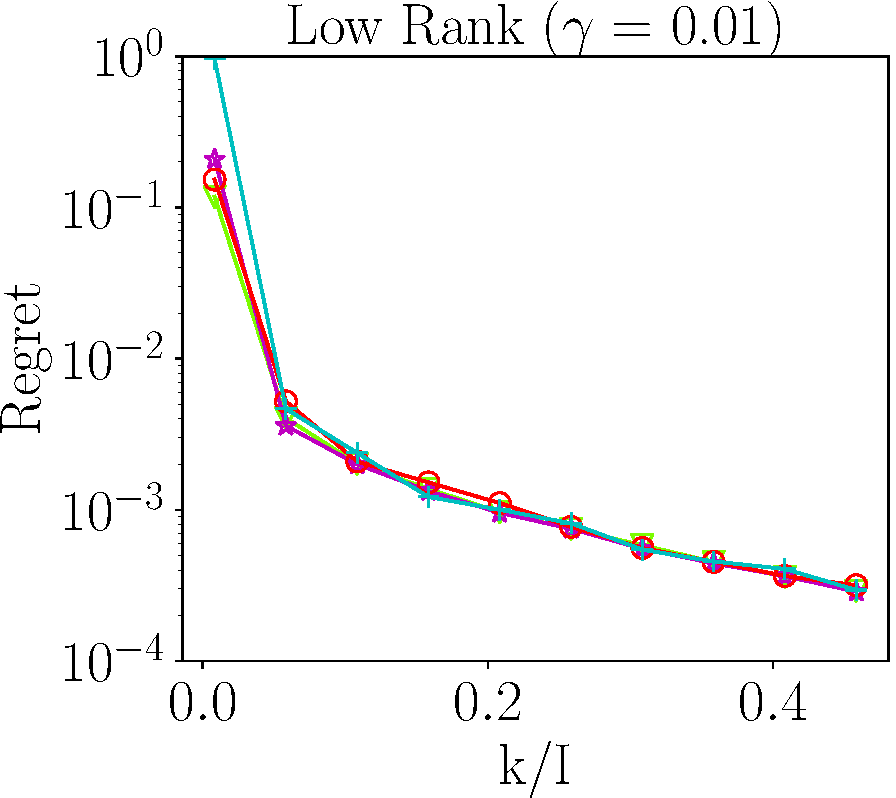
\includegraphics[scale = 0.24]{figure/fig2_lk_lnoise_600.pdf}
	\end{subfigure}
	\begin{subfigure}{0.3\textwidth}
		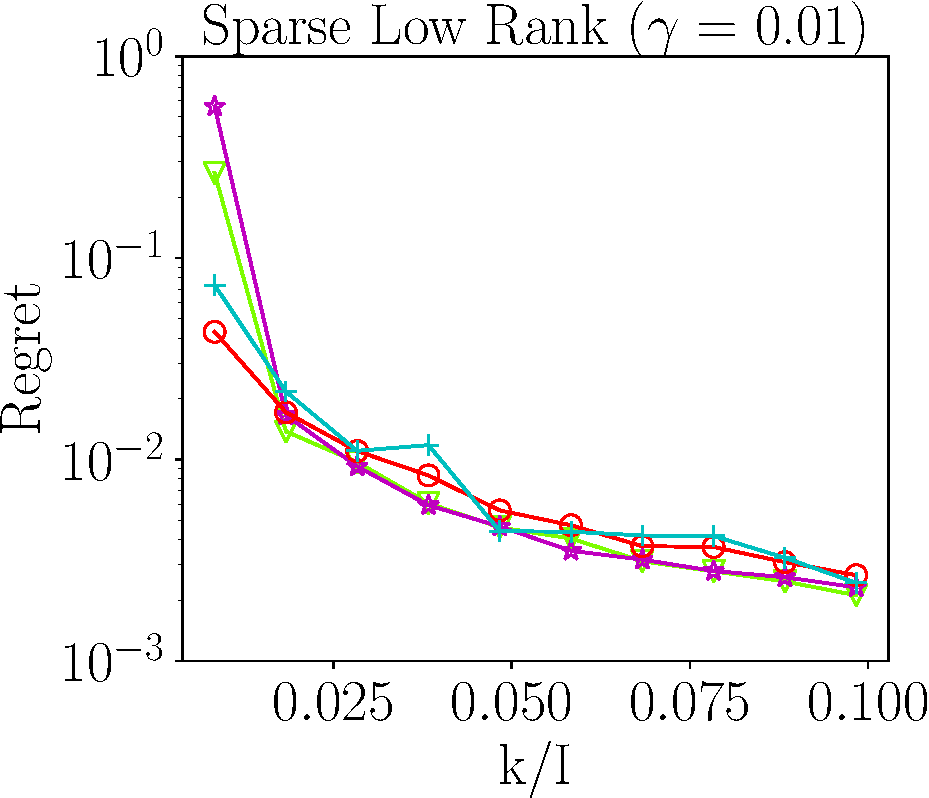
\includegraphics[scale = 0.24]{figure/fig2_slk_lnoise_600.pdf}
	\end{subfigure}
	\begin{subfigure}{0.3\textwidth}
		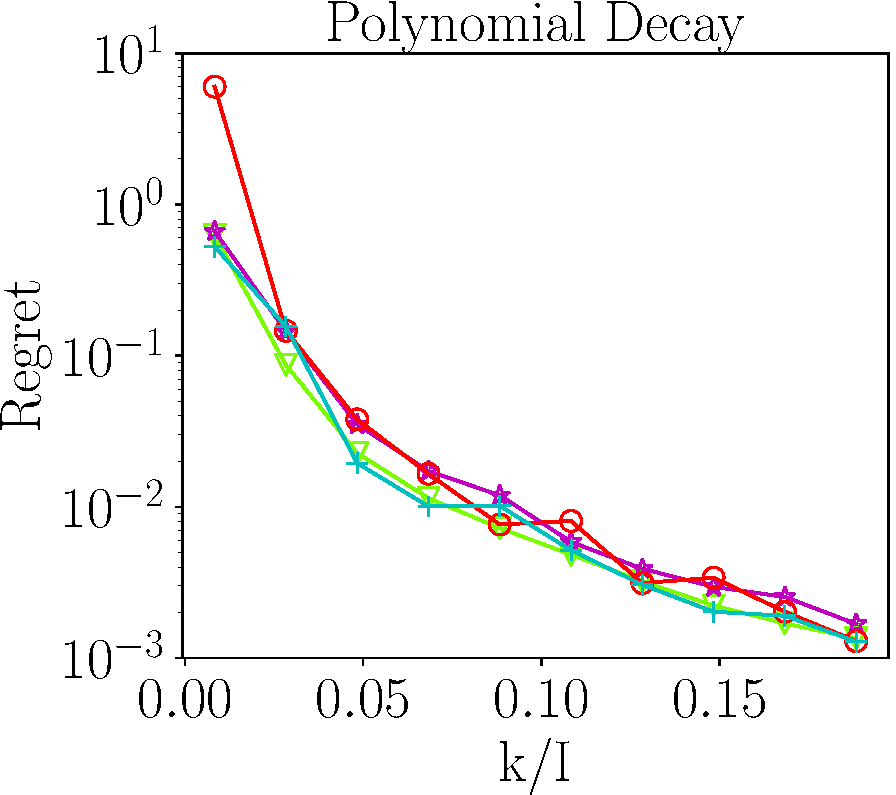
\includegraphics[scale = 0.24]{figure/fig2_spd_600.pdf}
	\end{subfigure}\\
	\begin{subfigure}{0.3\textwidth}
		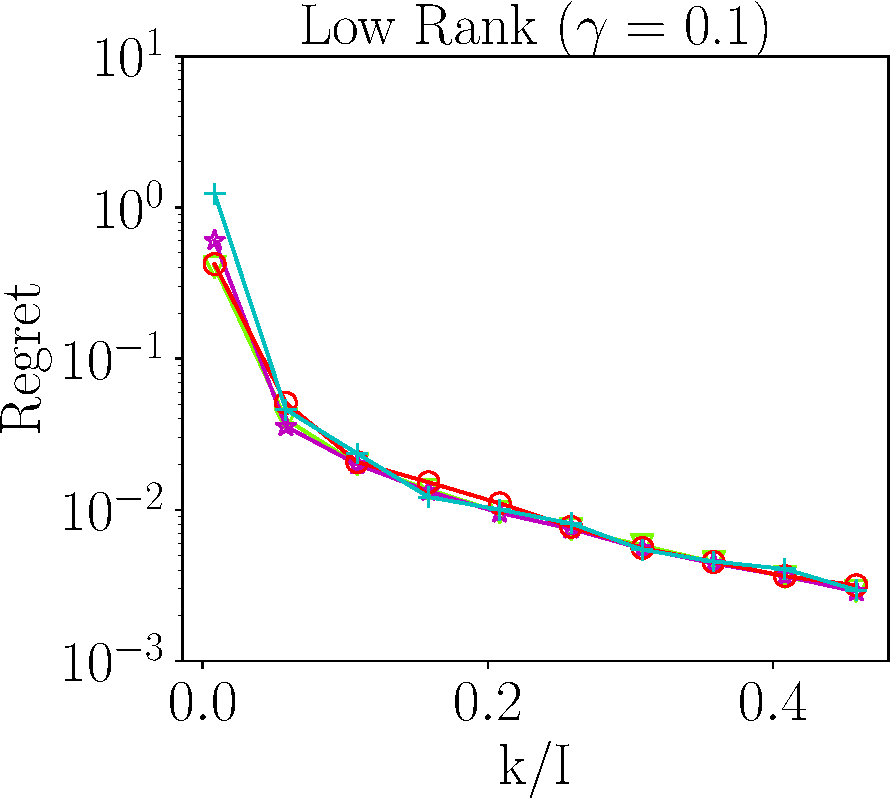
\includegraphics[scale = 0.24]{figure/fig2_lk_mnoise_600.pdf}
	\end{subfigure}
	\begin{subfigure}{0.5\textwidth}
		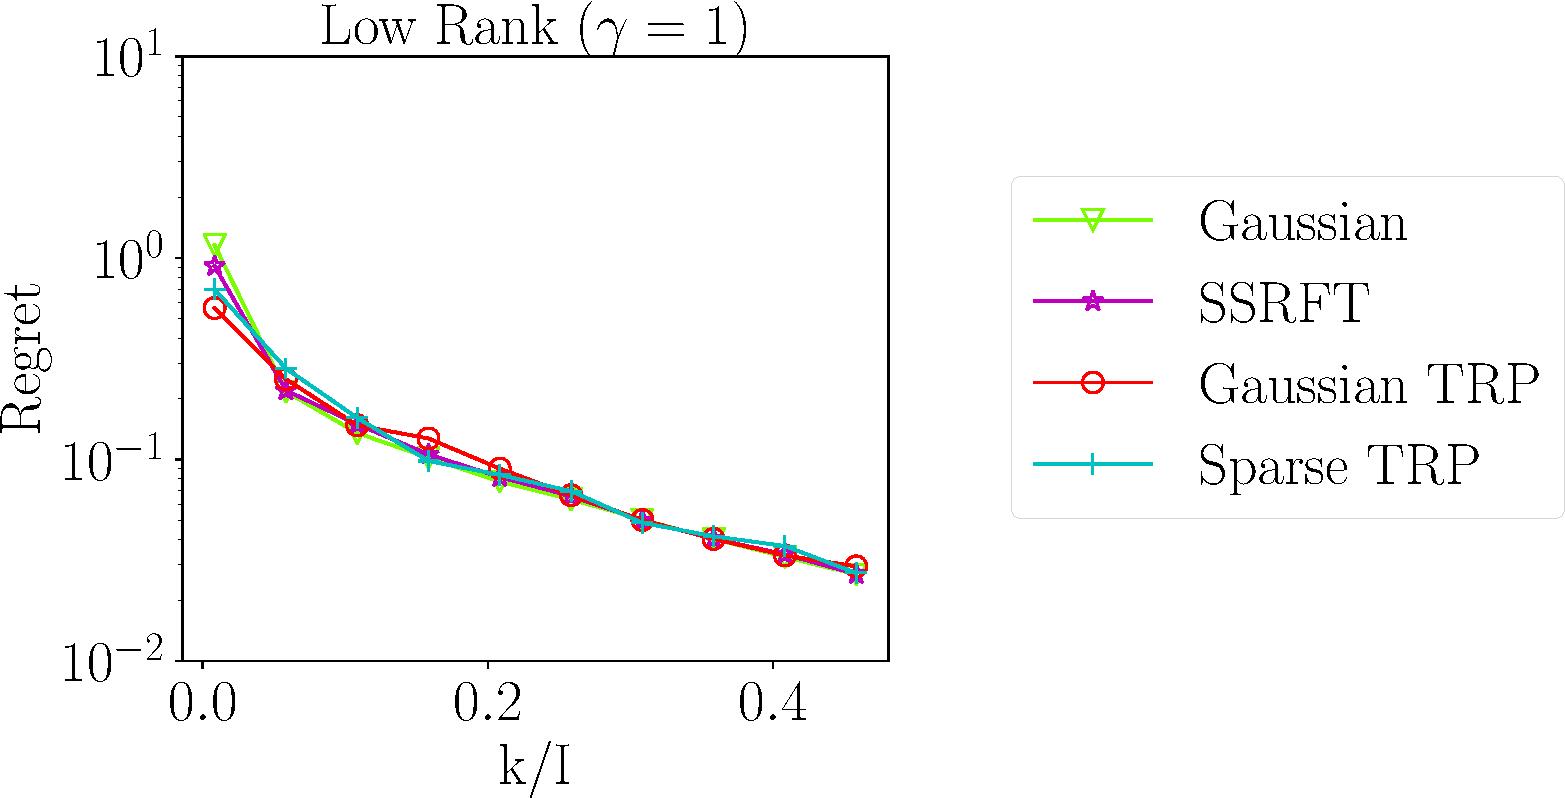
\includegraphics[scale = 0.24]{figure/fig2_lk_hnoise_600.pdf}
	\end{subfigure}
	\\
	\caption{\textit{Different DRMs perform similarly.}
		We approximate 3D synthetic tensors (see \ref{s-synthetic-data}) with $I = 600$,
		using our one-pass algorithm with $r = 5$ and varying $k$ ($s = 2k+1$),
		using a variety of DRMs in the Tucker sketch:
		Gaussian, SSRFT, Gaussian TRP, or Sparse TRP.
		\label{fig:vary-k-600}
	}
\end{figure}

\begin{figure}
	\centering
	\begin{subfigure}{0.3\textwidth}
		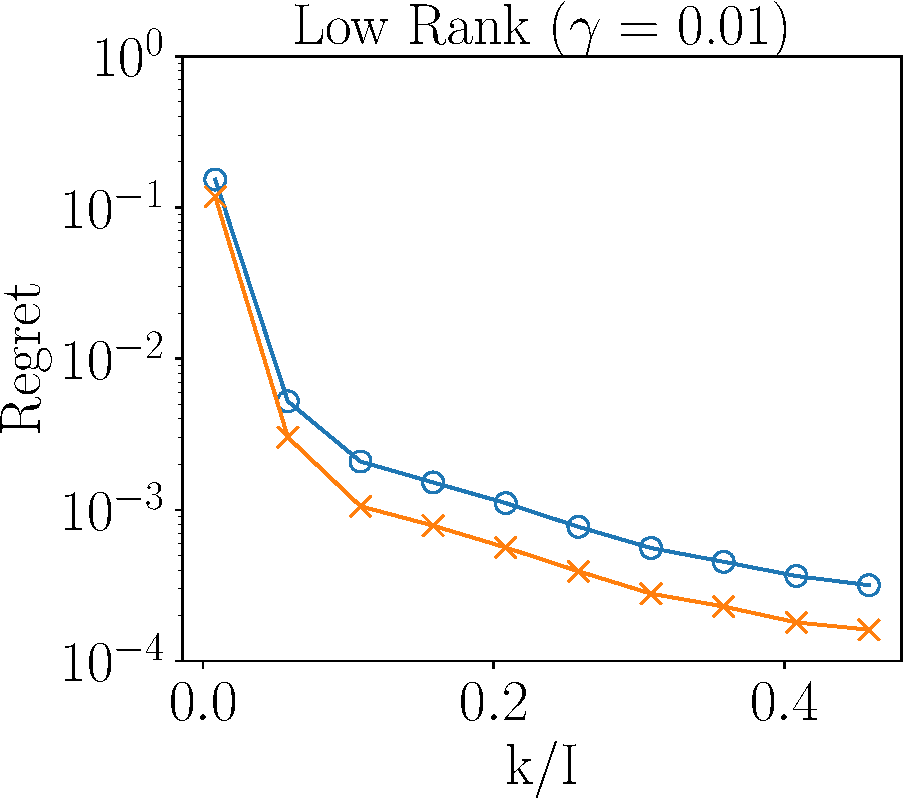
\includegraphics[scale = 0.24]{figure/fig3_lk_lnoise_600.pdf}
	\end{subfigure}
	\begin{subfigure}{0.3\textwidth}
		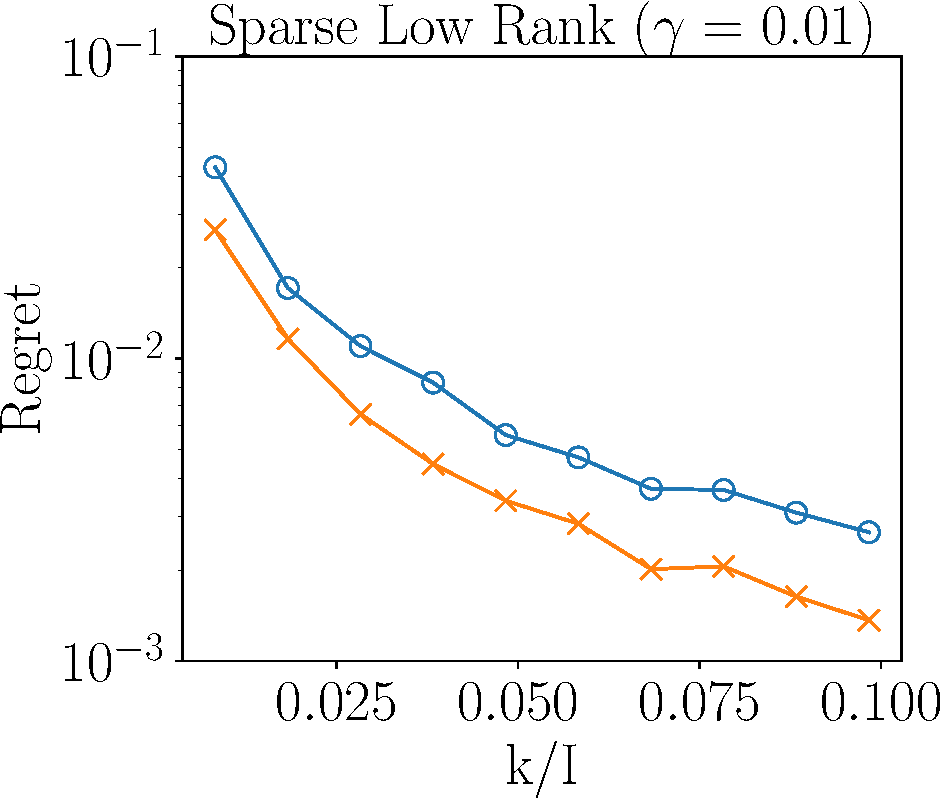
\includegraphics[scale = 0.24]{figure/fig3_slk_lnoise_600.pdf}
	\end{subfigure}
	\begin{subfigure}{0.3\textwidth}
		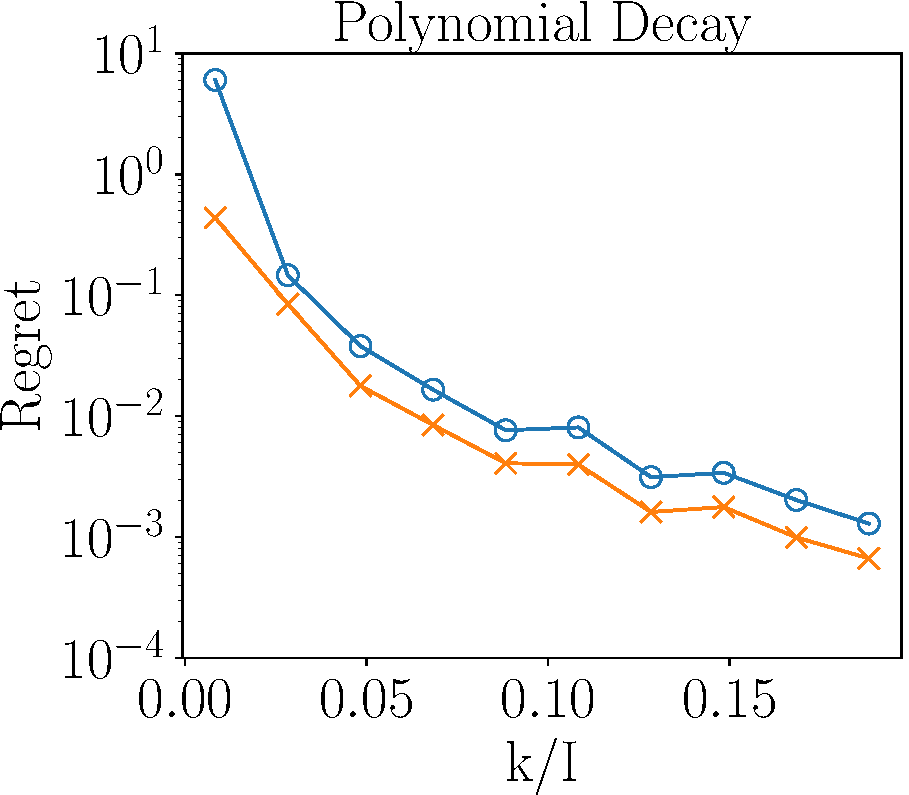
\includegraphics[scale = 0.24]{figure/fig3_spd_600.pdf}
	\end{subfigure}\\
	\begin{subfigure}{0.3\textwidth}
		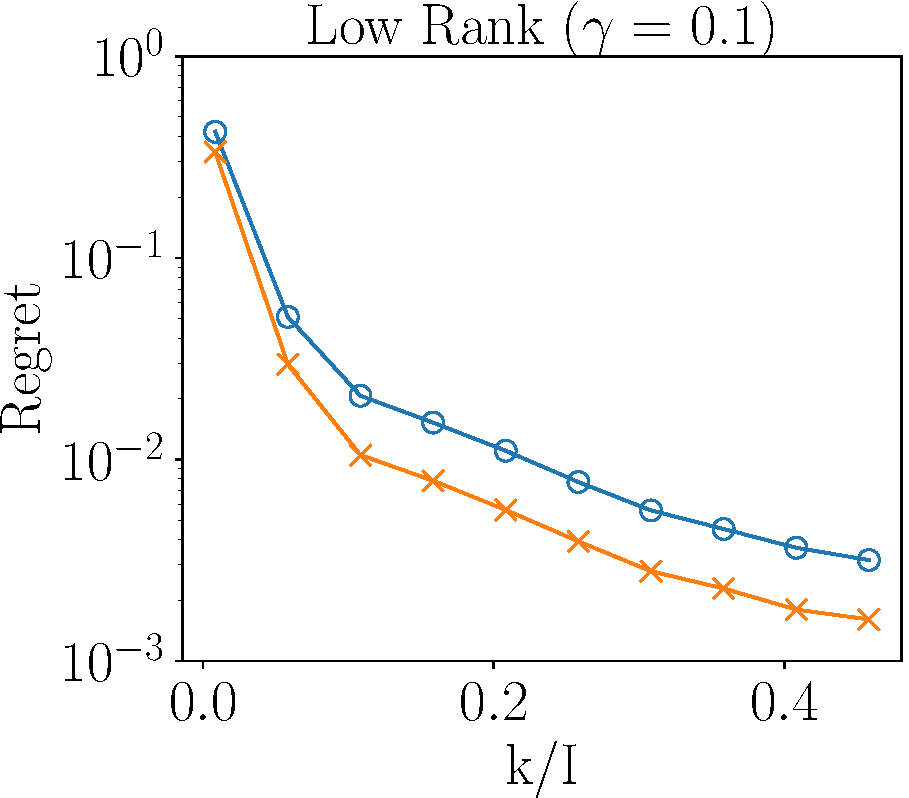
\includegraphics[scale = 0.24]{figure/fig3_lk_mnoise_600.pdf}
	\end{subfigure}
	\begin{subfigure}{0.55\textwidth}
		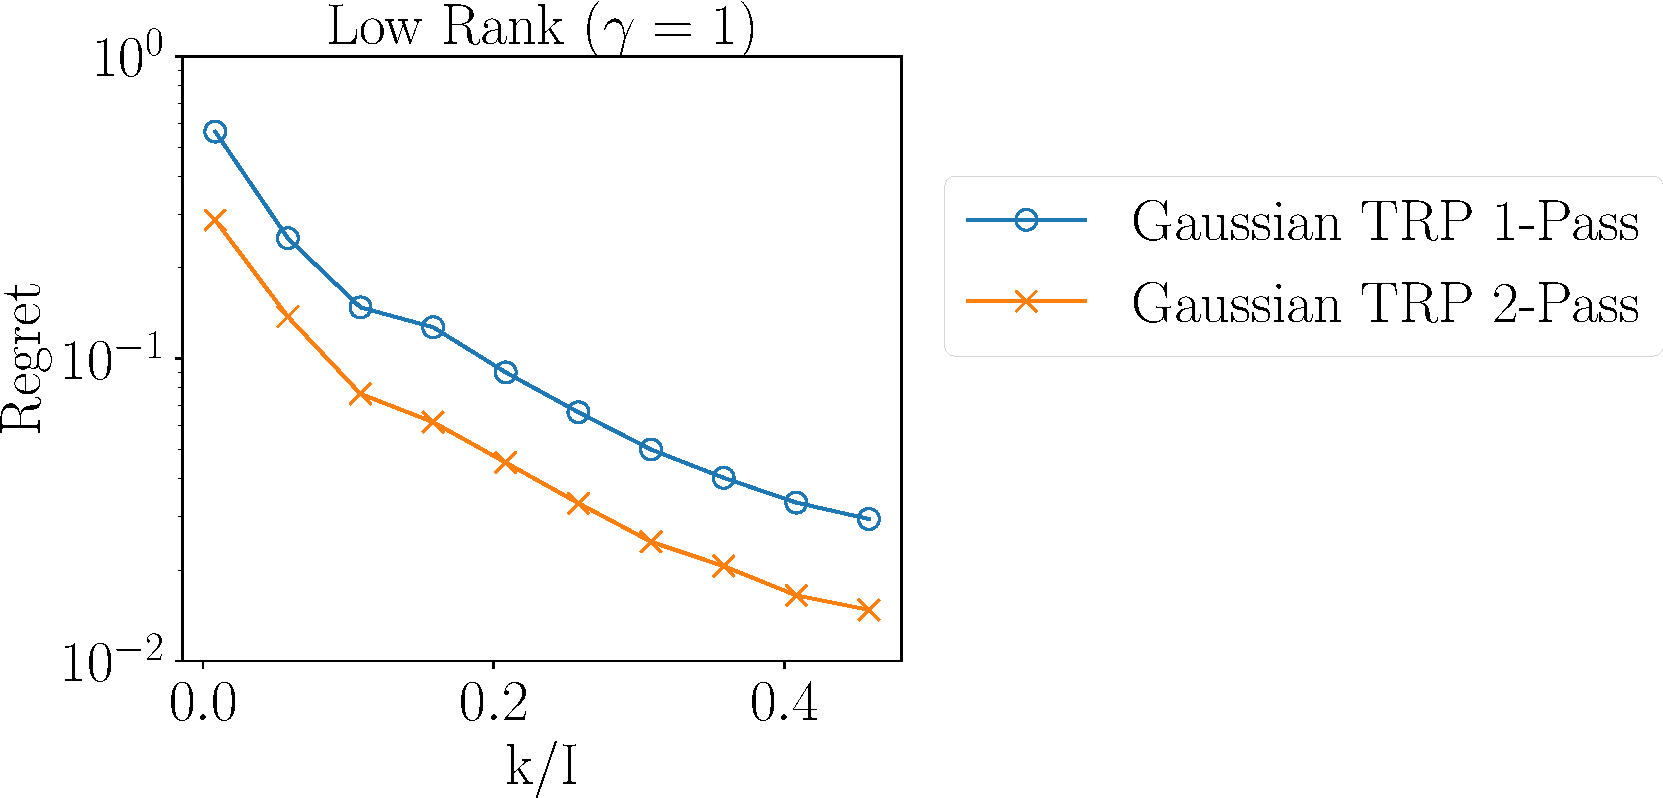
\includegraphics[scale = 0.24]{figure/fig3_lk_hnoise_600.pdf}
	\end{subfigure}
	\\
	\caption{\textit{Two-pass improves on one-pass.}
	We approximate 3D synthetic tensors (see \ref{s-synthetic-data}) with $I = 600$,
	using our one-pass and two-pass algorithms with $r = 5$ and varying $k$ ($s = 2k+1$),
	using the Gaussian TRP in the Tucker sketch.
	\label{fig:vary-k-600-compare}
  }
\end{figure}
In this section, we study the performance of our method.
We compare the performance of the method using various different
DRMs, including TRP.
We also compare our method with the algorithm proposed by \cite{malik2018low}
to show that for the same storage budget, our method produces better approximations.
Our two-pass algorithm outperforms the one-pass version, as expected.
(Contrast this to \cite{malik2018low}, where the multi-pass method
performs less well than the one-pass version.)
% Experiments on real data show effective compression
% can be achieved in a single pass.

\begin{figure}
	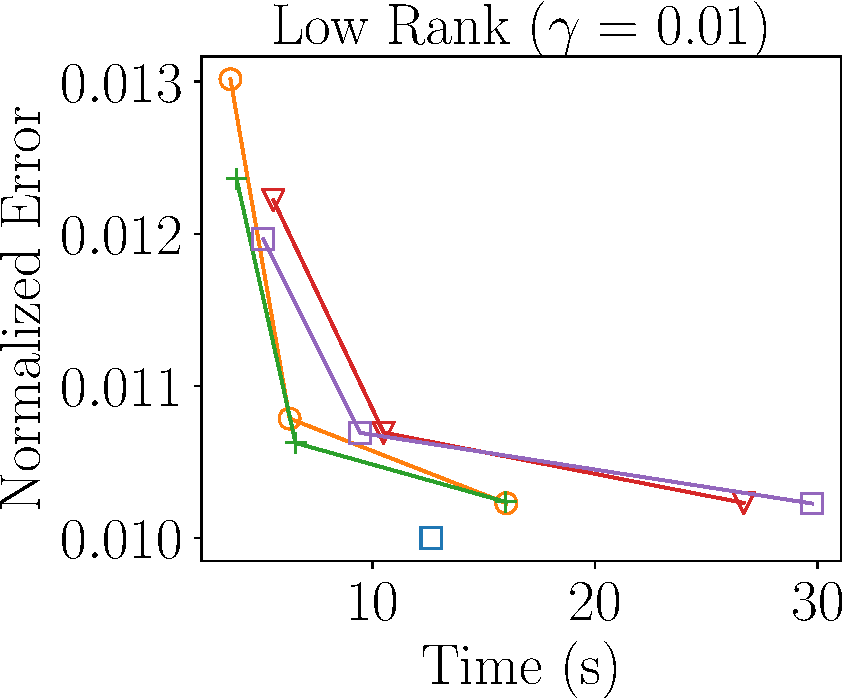
\includegraphics[height=2.5cm]{figure/lk_1pass_time.pdf}
	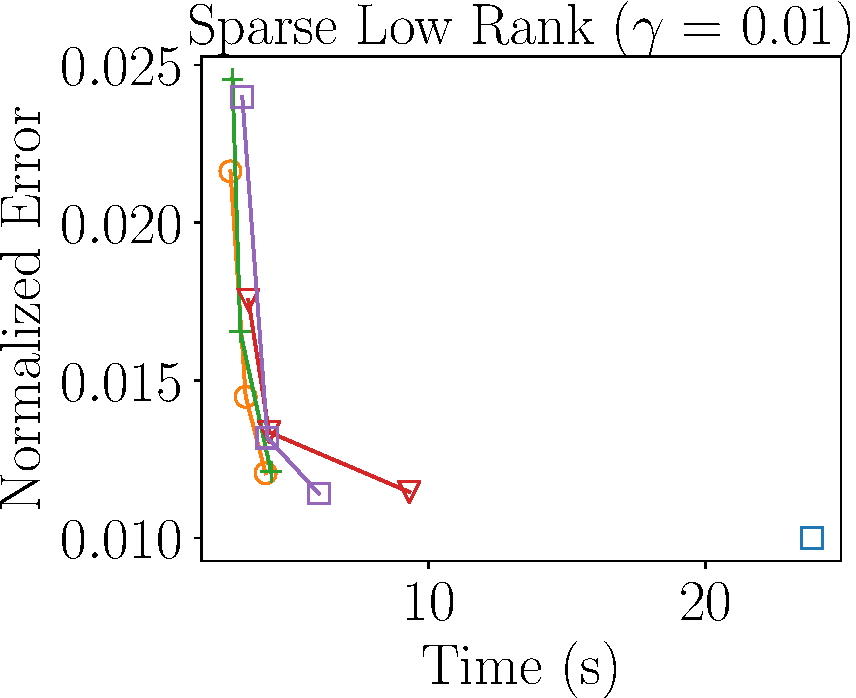
\includegraphics[height=2.5cm]{figure/slk_1pass_time.pdf}
	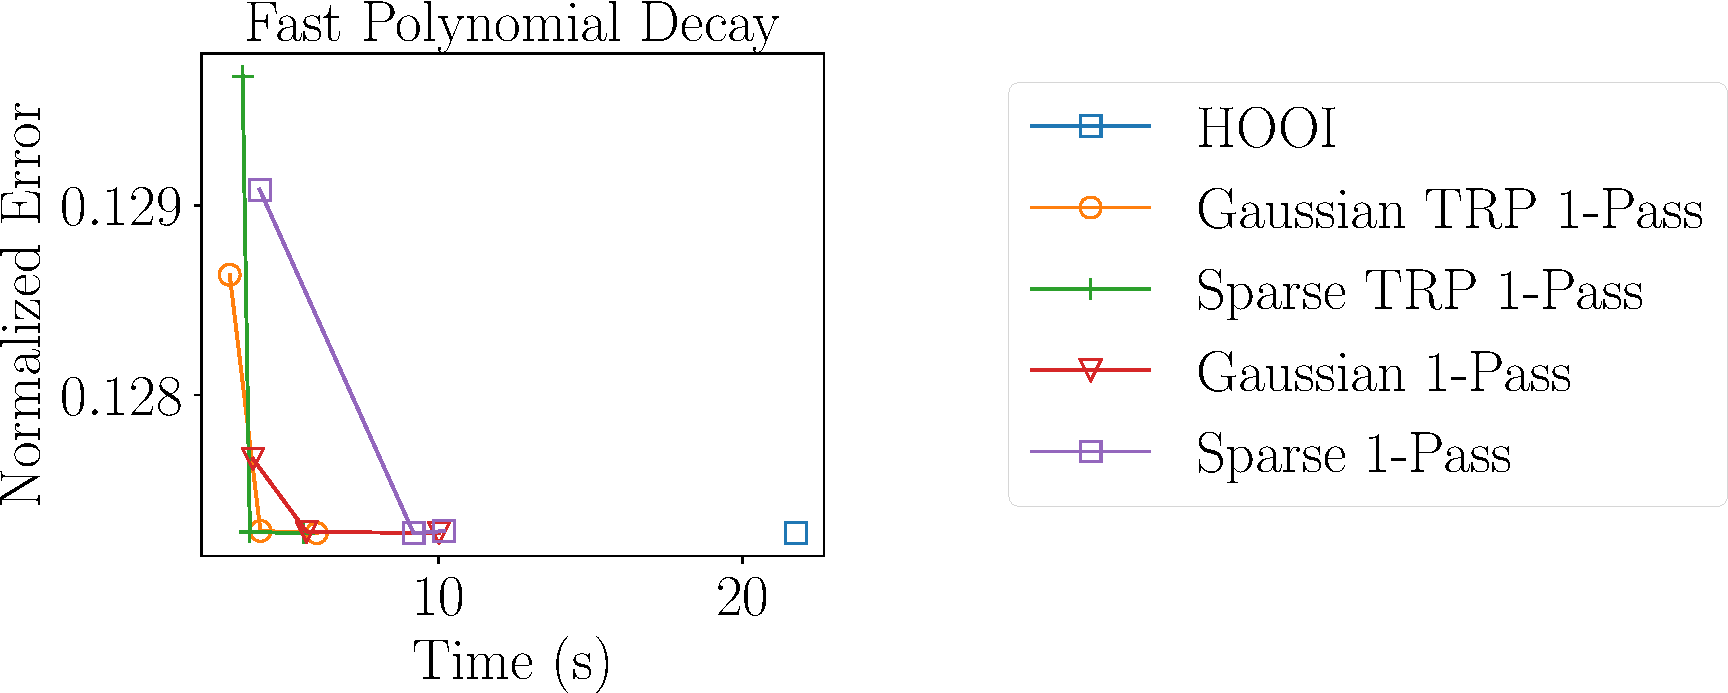
\includegraphics[height=2.5cm]{figure/fpd_1pass_time.pdf}\\
	\centering
	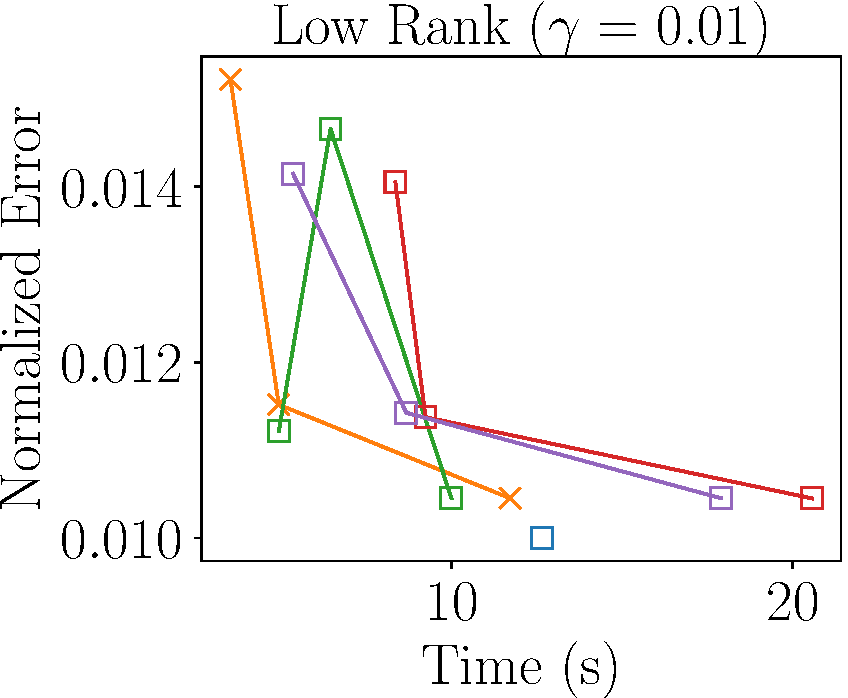
\includegraphics[height=2.5cm]{figure/lk_2pass_time.pdf}
	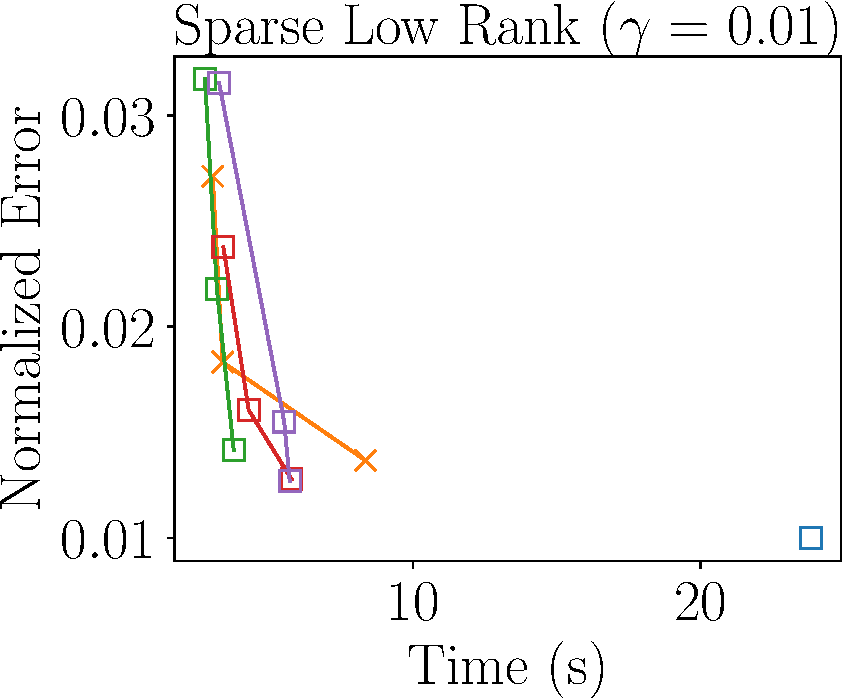
\includegraphics[height=2.5cm]{figure/slk_2pass_time.pdf}
	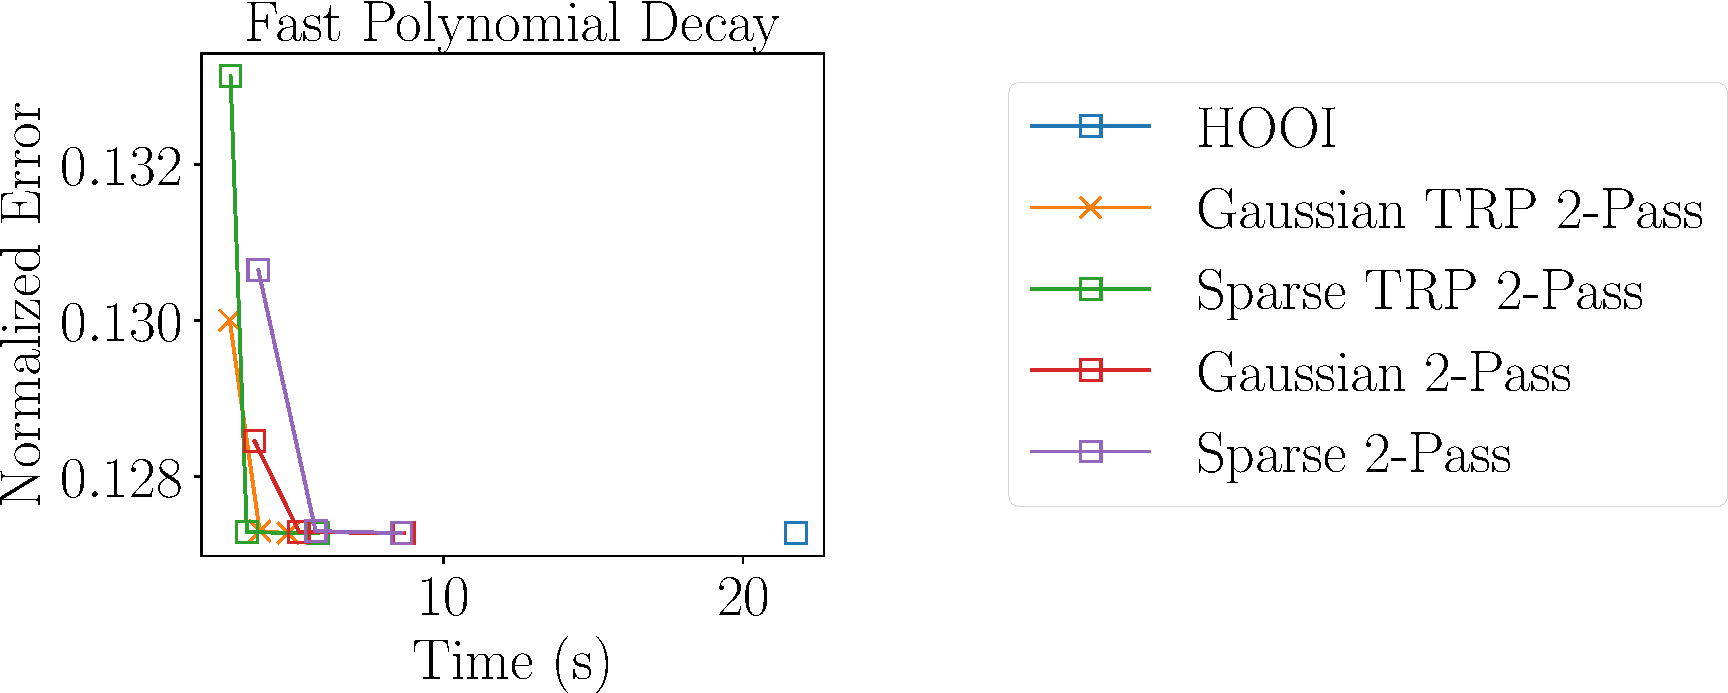
\includegraphics[height=2.5cm]{figure/fpd_2pass_time.pdf}\\
	\centering
	\caption{
	\textit{Faster approximations.}
	We approximate 3D synthetic tensors with $I = 600$ generated
	as described in \ref{s-synthetic-data},
	using HOOI and our one-pass and two-pass algorithms with $r = 5$
	for a few different $k$ ($s = 2k+1$).
	% We try several DRMs in the Tucker sketch:
	% Gaussian, Sparse, Gaussian TRP, and Sparse TRP.
	% Tradeoff between Time and Relative Error: We compare HOOI and our two algorithms across different random maps with $I=600, \mathbf{r}=(5,5,5)$, $\gamma = 0.01$.
}\label{fig:run_time}
\end{figure}

We evaluate the experimental results using two metrics:
\[
% \begin{array}{lc}
% \mbox{normalized error:} & \frac{\|\T{X} - \hat{\T{X}}\|_F}{\|\T{X}\|_F} \\
% \mbox{relative error:} & \frac{\|\T{X} - \hat{\T{X}}\|}{\|\T{X} - \T{X}_\text{HOOI}\|} - 1 \\
% \mbox{regret:} & \frac{\|\T{X} - \hat{\T{X}}\|_F}{\|\T{X}\|_F} -
%                    \frac{\|\T{X} - \T{X}_\text{HOOI}\|_F}{\|\T{X}\|_F}.
% \end{array}
\begin{array}{lc}
\mbox{normalized error:} & \|\T{X} - \hat{\T{X}}\|_F / \|\T{X}\|_F \\
% \mbox{relative error:} & \nicefrac{\|\T{X} - \hat{\T{X}}\|}{\|\T{X} - \T{X}_\text{HOOI}\|} - 1 \\
\mbox{regret:} & \left(\|\T{X} - \hat{\T{X}}\|_F - \|\T{X} - \T{X}_\text{HOOI}\|_F \right) / \|\T{X}\|_F.
\end{array}
\]
The normalized error measures the fraction of the energy in $\T{X}$
captured by the approximation.
The regret measures the increase in normalized error due to
using the approximation $\hat{\T{X}}$ rather than using $\T{X}_\text{HOOI}$.
The relative error measures the decrease in performance relative to HOOI.
%\mnote{Joel says: I prefer to call this the "normalized" error, rather than the "relative" error. The former scales the error so it should usually be less than one. The second compares the error with the "optimum" error: ||X - hat{X}|| / ||X - HOOI(X)|| - 1.You might consider whether you actually want the latter.}
The normalized error of a rank $\V{r}$ Tucker approximation $\hat{X}$
is always positive when $\T{X}$ has a larger rank.
In general, we find our proposed methods approaches the performance of HOOI
for large enough storage budgets.

We ran all experiments on a server with 128 Intel\textsuperscript{\textregistered} Xeon\textsuperscript{\textregistered} E7-4850 v4 2.10GHz CPU cores and 1056GB memory.
The code for our method is available at an anonymous Github repository \url{https://github.com/tensorsketch/tensorsketch}.

\subsection{Synthetic experiments}\label{s-synthetic-data}
All synthetic experiments use an input tensor with equal side lengths $I$.
We consider three different data generation schemes:
\begin{itemize}
\item \emph{Low rank + noise.} Generate a core tensor $\T{C} \in \mathbb{R}^{r^N}$ with entries drawn from $\mathrm{Unif}([0,1])$.
  Independently generate $N$ orthogonal factor matrices
  $\mathbf{A}_1, \dots, \mathbf{A}_N \in \mathbb{R}^{r \times I}$.
	Define $\T{X}^\natural = \T{C} \times_1 \mathbf{A}_1 \cdots \times_N \mathbf{A}_N$
	and the noise parameter $\gamma > 0$.
	Generate an input tensor as
	$\T{X} = \T{X}^\natural + (\gamma \|\T{X}^\natural\|_F / I^{N/2})\T{\epsilon}$
	where the noise $\T{\epsilon}$ has i.i.d. $\mathcal{N}(0,1)$ entries.
	% by orthogonalizing random matrices with each entry drawn from $\mathcal{N}(0,1)$.
%   The input tensor is
%  \[
% \T{X} = \T{C} \times_1 \mathbf{A}_1 \cdots \times_N \mathbf{A}_N + \sqrt{\frac{\gamma^2 \cdot \|\T{X}^\natural\|_F^2}{I^N}} \mathcal{N}(0,1),
% \]
% where $\T{X}^\natural = \T{C} \times_1 \mathbf{A}_1 \cdots \times_N \mathbf{A}_N$.
% Here $1/\gamma^2$ measures the signal-to-noise ratio.
% In the simulations, we use three different noise levels: $\gamma = 0.01, 0.1, 1$.
\item \emph{Sparse low rank + noise.} We construct the input tensor $\T{X}$ as above (Low Rank + Noise),
but with sparse factor matrices $\mathbf{A}_n$:
If $\delta_n$ is the sparsity (proportion of non-zero elements) of $\mathbf{A}_n$,
then the sparsity of the true signal $\T{X}^\natural$ is $\prod_{n=1}^N \delta_n$.
%We set the noise $\gamma = 0.01$ (Results for $\gamma = 0.1,0.1$ are empirically analogous to the previous setting).
We use $\delta_n = 0.2$ unless otherwise specified.
\item \emph{Polynomial decay.} We construct the input tensor $\T{X}$ as
  \begin{equation*}
      \T{X} = \mathop{\textbf{superdiag}}(1,\dots,1, 2^{-t},3^{-t},\dots, (I-r)^{-t}).
  \end{equation*}
  The first $r$ entries are 1.
	Recall $\mathop{\textbf{superdiag}}$ converts a vector to $N$ dimensional superdiagonal tensor.
  Our experiments use $t = 1$ (geometric decay).
\end{itemize}

\subsubsection{Different dimension reduction maps perform similarly}
Our first experiment investigates the performance of our one-pass fixed-rank algorithm
as the sketch size (and hence, required storage) varies,
for several types of dimension reductions maps, including Gaussian, SSRFT, Gaussian TRP, and Sparse TRP.
We generate synthetic data as described above with $\mathbf{r} = (5,5,5), I = 600$.
\ref{fig:vary-k-600} shows the rank-$\mathbf{r}$ approximation error
as a function of the compression factor $k/I$.
\ifdefined \issupplement
(Results for other input tensors appear in the supplement.)
\else
(Results for other input tensors are presented as
\ref{fig:vary-k-400-app} and \ref{fig:vary-k-200-app} in \ref{appendix:more_result}.)
\fi
We see that the log relative error for our one-pass algorithm
converges to that of HOOI as $k$ increases for all input tensors.
In the low rank case, the convergence rate is lower for higher noise levels.
In general, the performance for different maps are approximately the same,
although our theory only pertains to the Gaussian map.
% In the low-rank sparse case and low-rank high noise case,
% the Gaussian TRP outperforms the Gaussian, possibly due to the implicit bias from the Khatri-Rao structure.

We evaluate the run time for HOOI and our two algorithms with several different DRMs in \ref{fig:run_time}. We can see that the one-pass algorithm is always slightly faster than the two-pass algorithm. The TRP generally provides a modest speedup in addition to the memory advantage.
Both our one-pass and two-pass algorithms achieve nearly the accuracy of HOOI,
and are usually much faster. % for tensors that are not exactly low rank.

\begin{figure}
	\centering
	\begin{subfigure}{0.3\textwidth}
		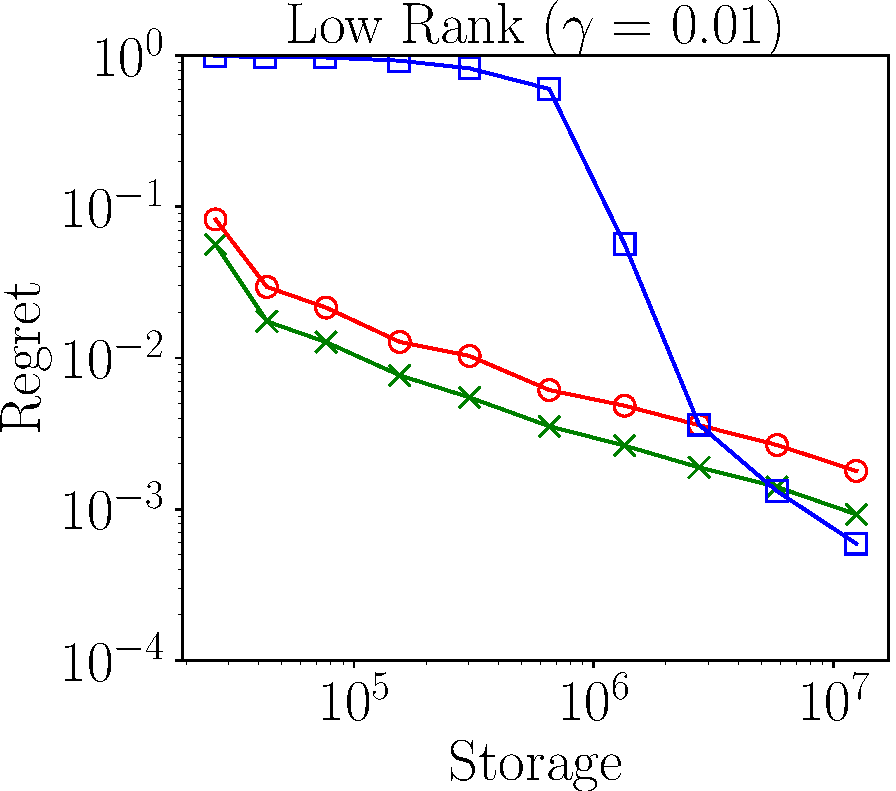
\includegraphics[scale = 0.24]{figure/fig1_lk_lnoise.pdf}
	\end{subfigure}
	\begin{subfigure}{0.3\textwidth}
		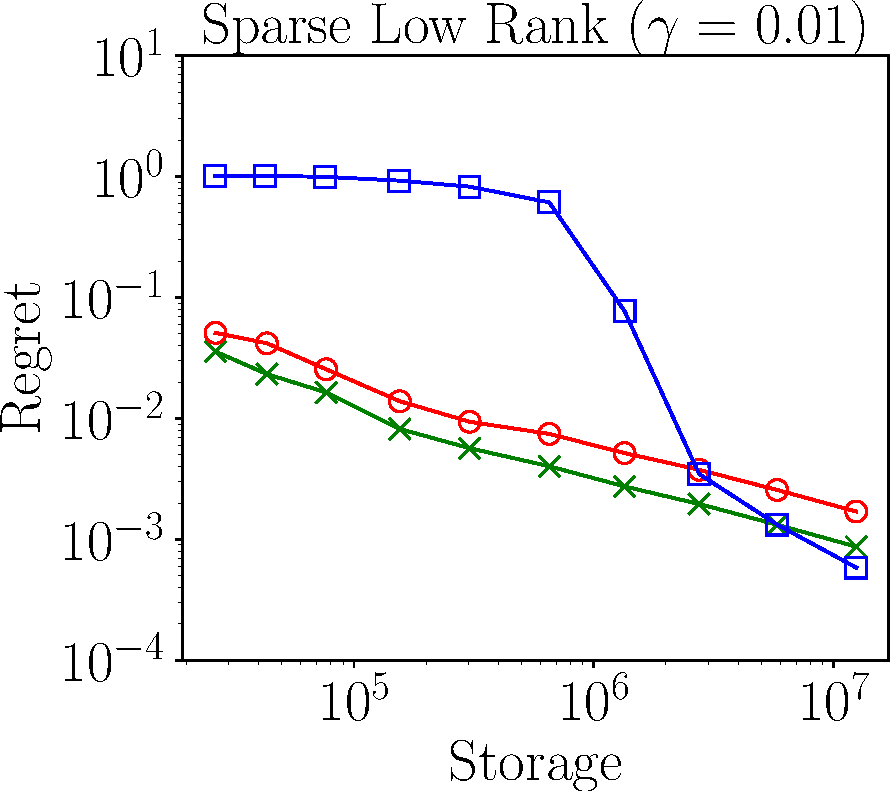
\includegraphics[scale = 0.24]{figure/fig1_slk_lnoise.pdf}
	\end{subfigure}
	\begin{subfigure}{0.3\textwidth}
		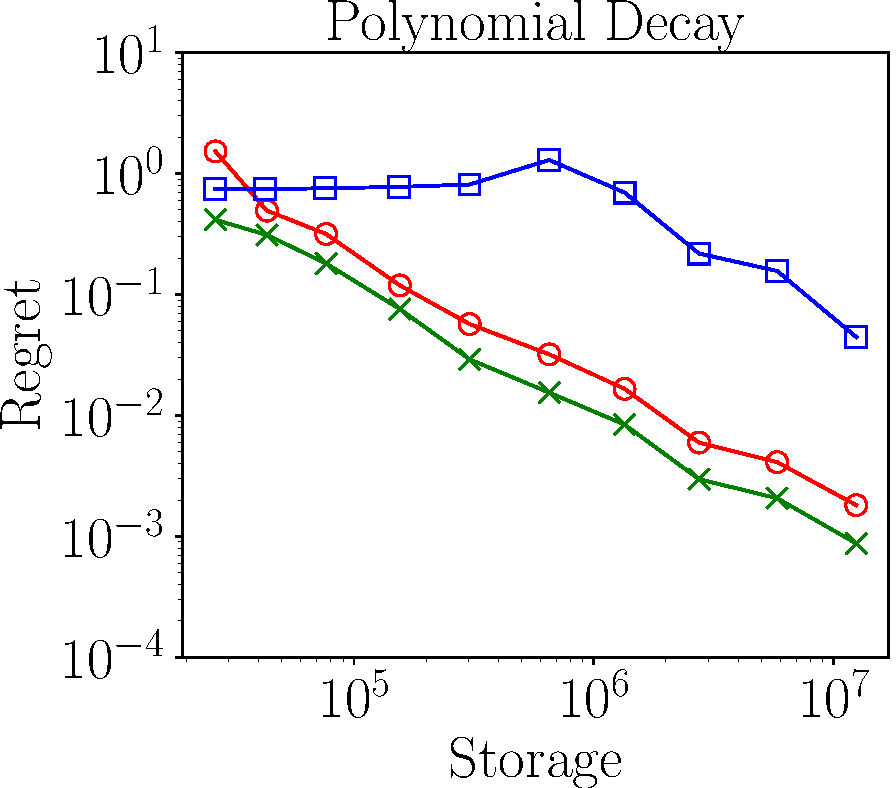
\includegraphics[scale = 0.24]{figure/fig1_spd.pdf}
	\end{subfigure}\\
	\begin{subfigure}{0.3\textwidth}
		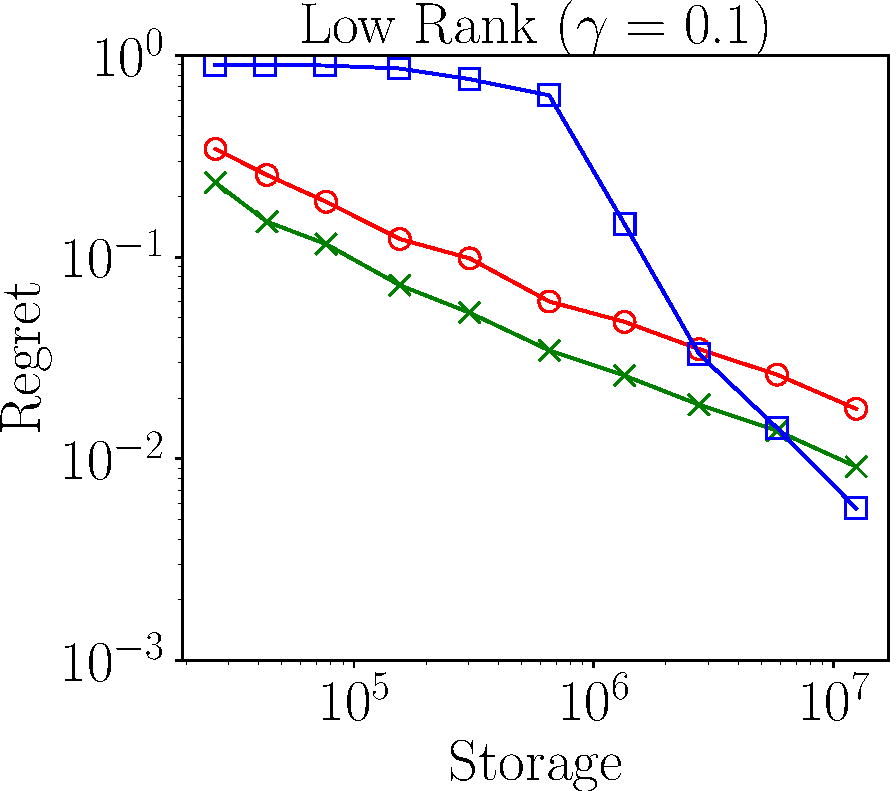
\includegraphics[scale = 0.24]{figure/fig1_lk_mnoise.pdf}
	\end{subfigure}
	\begin{subfigure}{0.43\textwidth}
		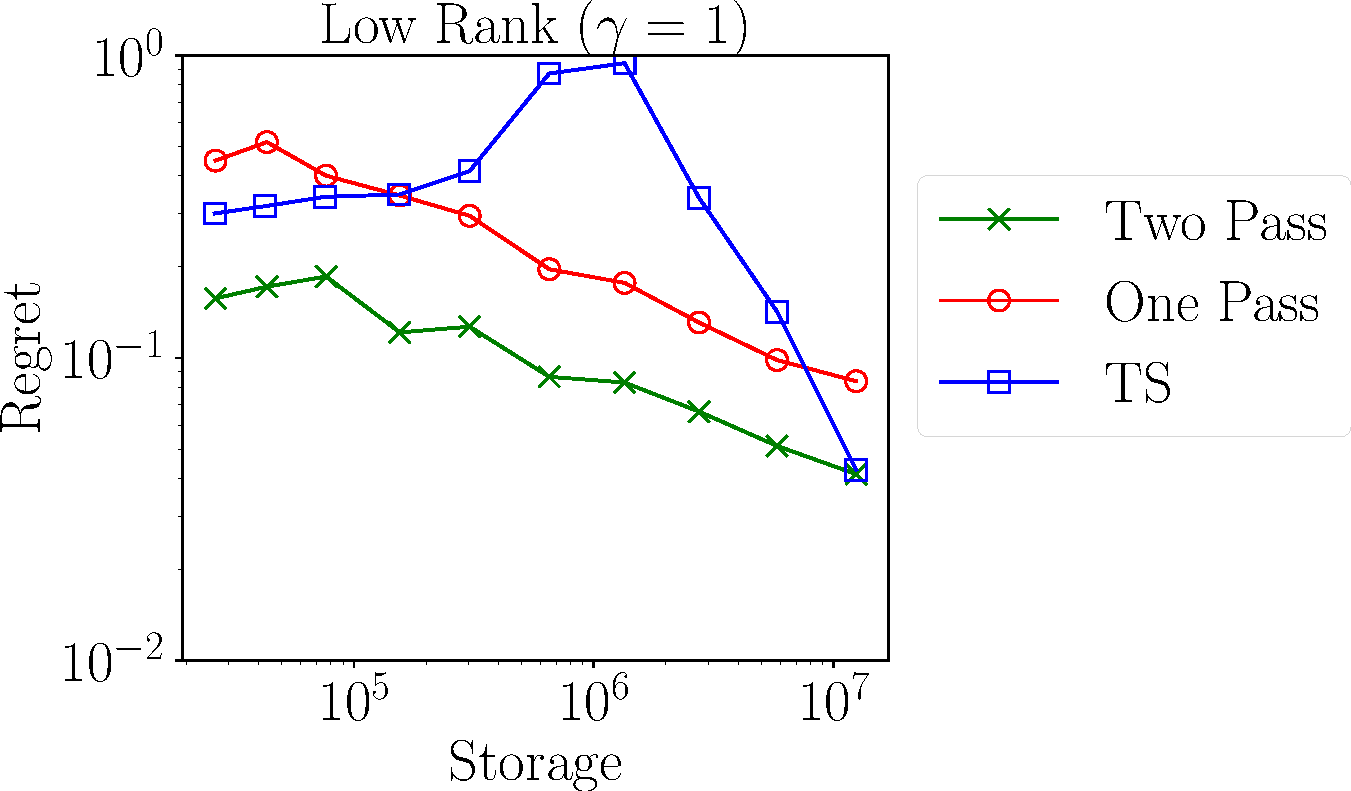
\includegraphics[scale = 0.24]{figure/fig1_lk_hnoise.pdf}
	\end{subfigure}\\
	\caption{\textit{Approximations improve with more memory: synthetic data.}
	We approximate 3D synthetic tensors (see \ref{s-synthetic-data}) with $I = 300$,
	using  T.-TS and our one-pass and two-pass algorithms
	with the Gaussian TRP to produce approximations with equal ranks $r=10$.
	Notice every marker on the plot corresponds to a 2700$\times$ compression!}\label{fig:vary-memory}
	% The total memory use is determined by the sketch size,
	% computed as $((2k+1)^N + kIN)$ for the one-pass method and $(Kr^{2N}+Kr^{2N-2})$ for T.-TS.
\end{figure}

\begin{figure}
	\centering
	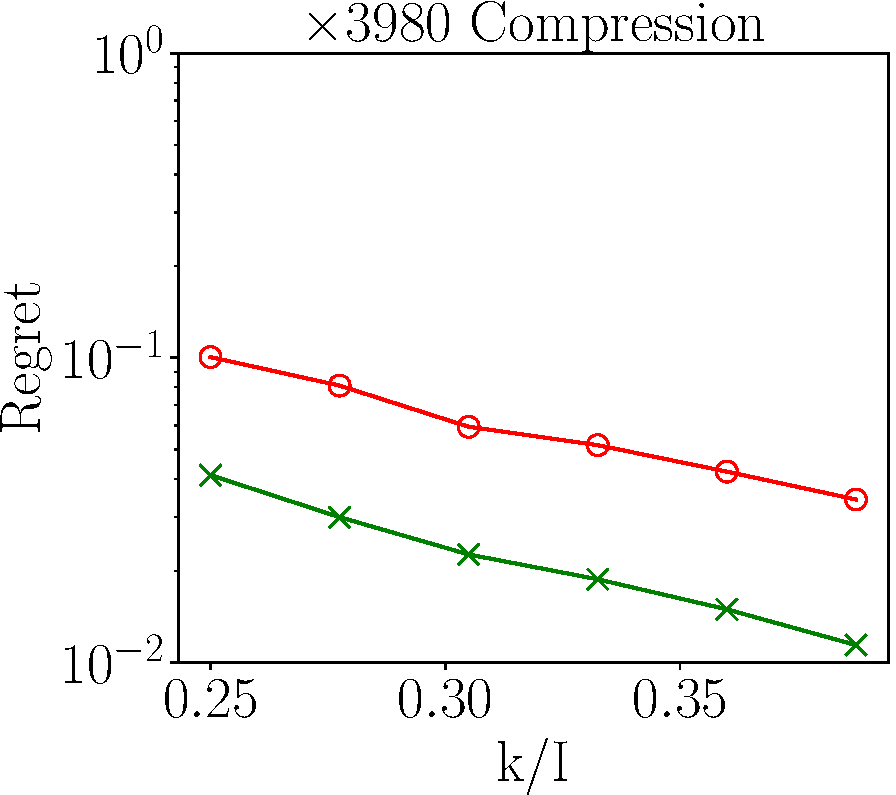
\includegraphics[height=2.9cm]{figure/multi_ABSORB_frk8.pdf}
	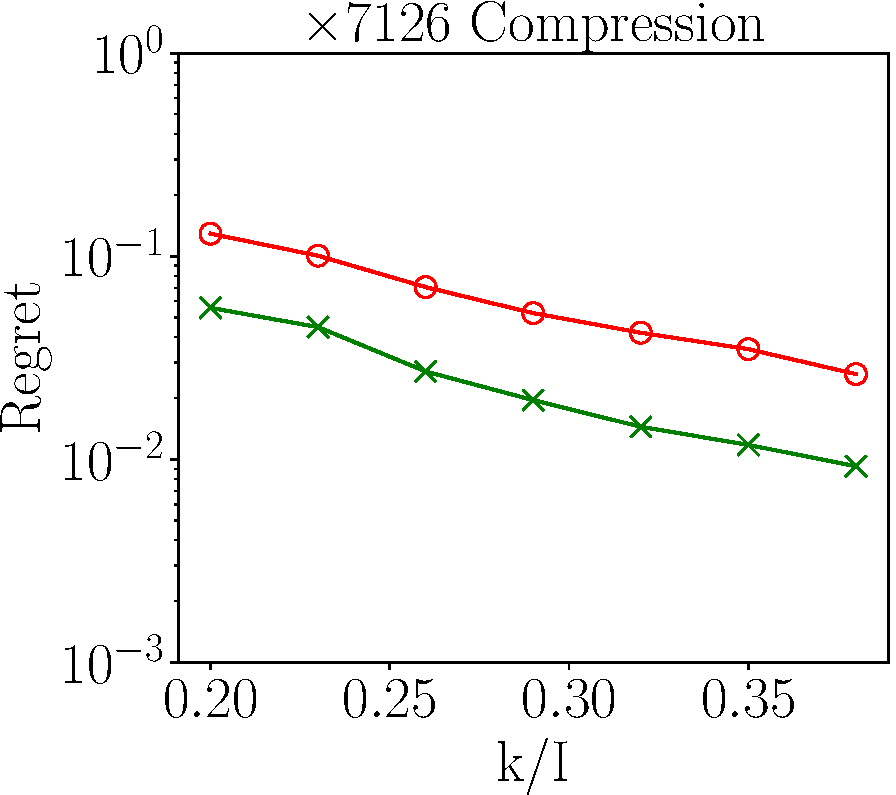
\includegraphics[height=2.9cm]{figure/multi_ABSORB_frk10.pdf}
	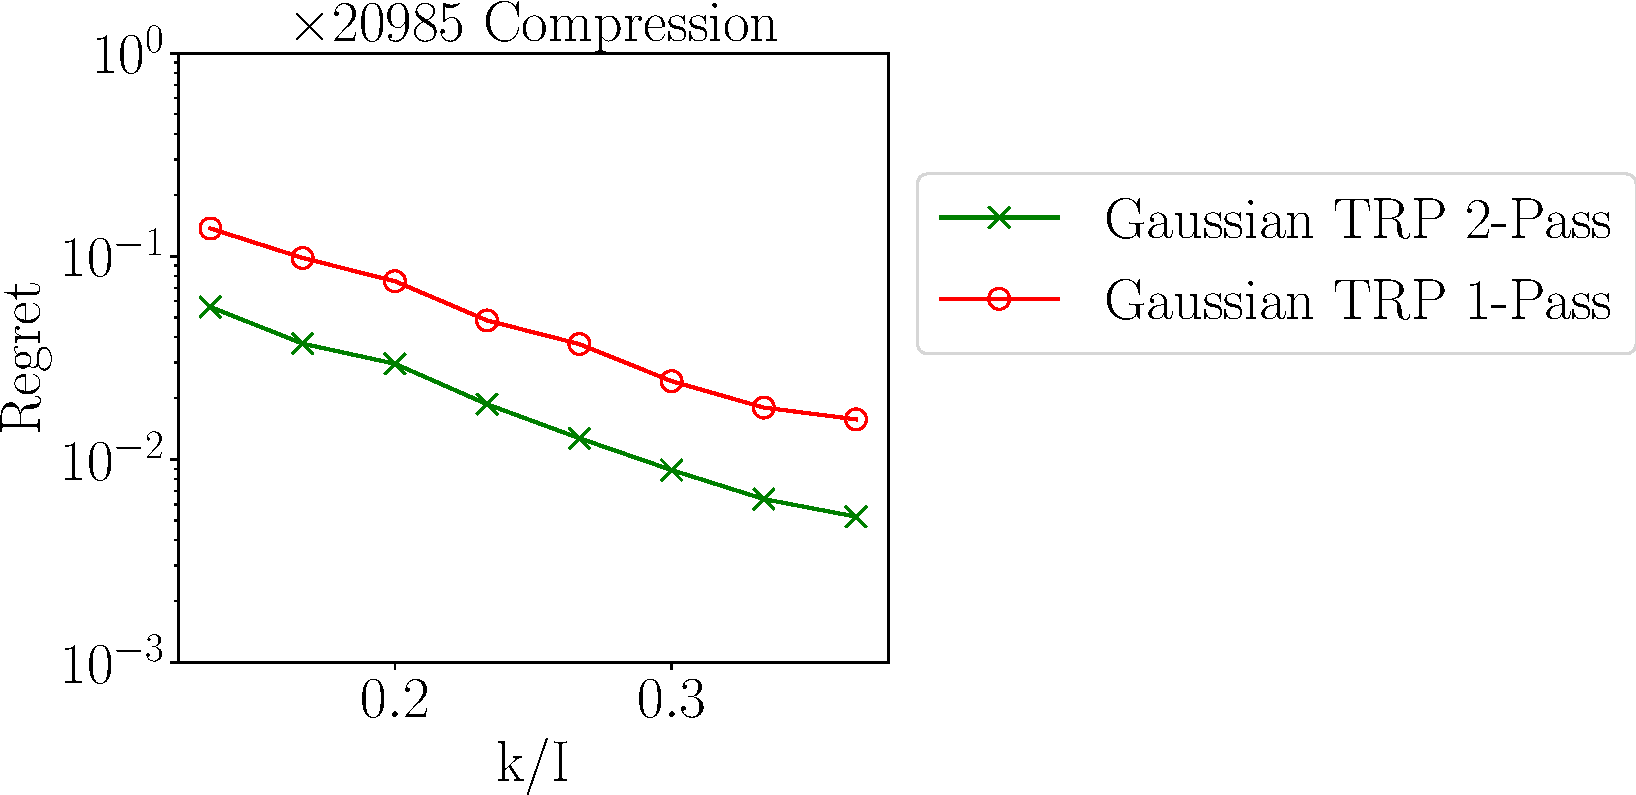
\includegraphics[height=2.9cm]{figure/multi_ABSORB_frk15.pdf}\\
	\textbf{Aerosol Absorption}\\~\\
	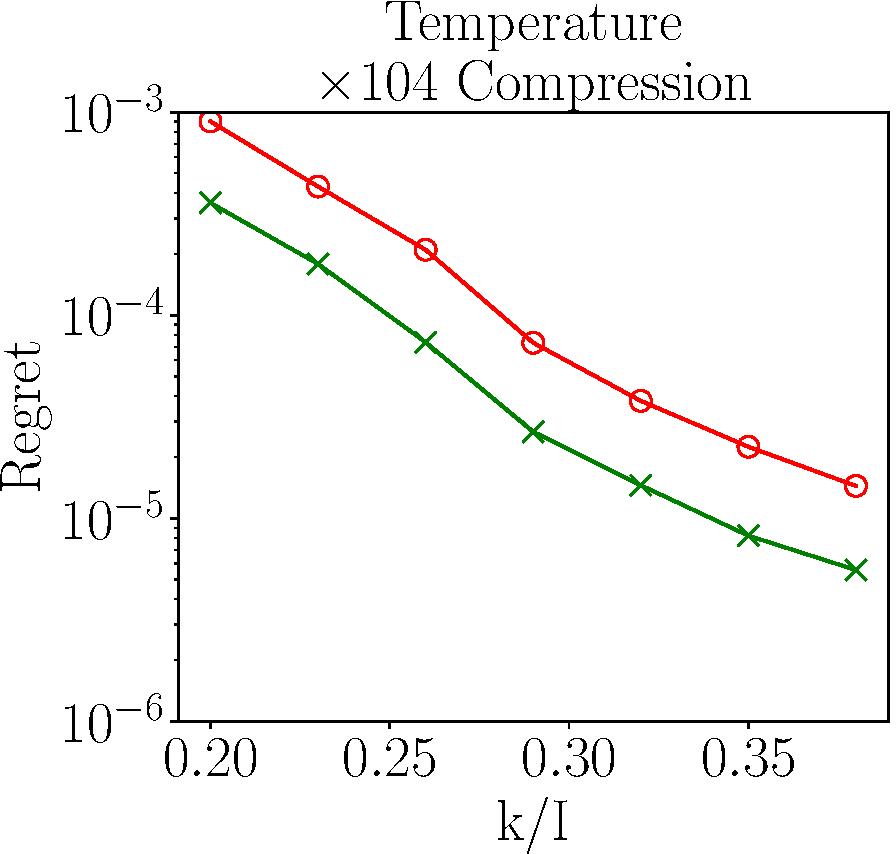
\includegraphics[height=2.9cm]{figure/multi_T_frk10.pdf}
	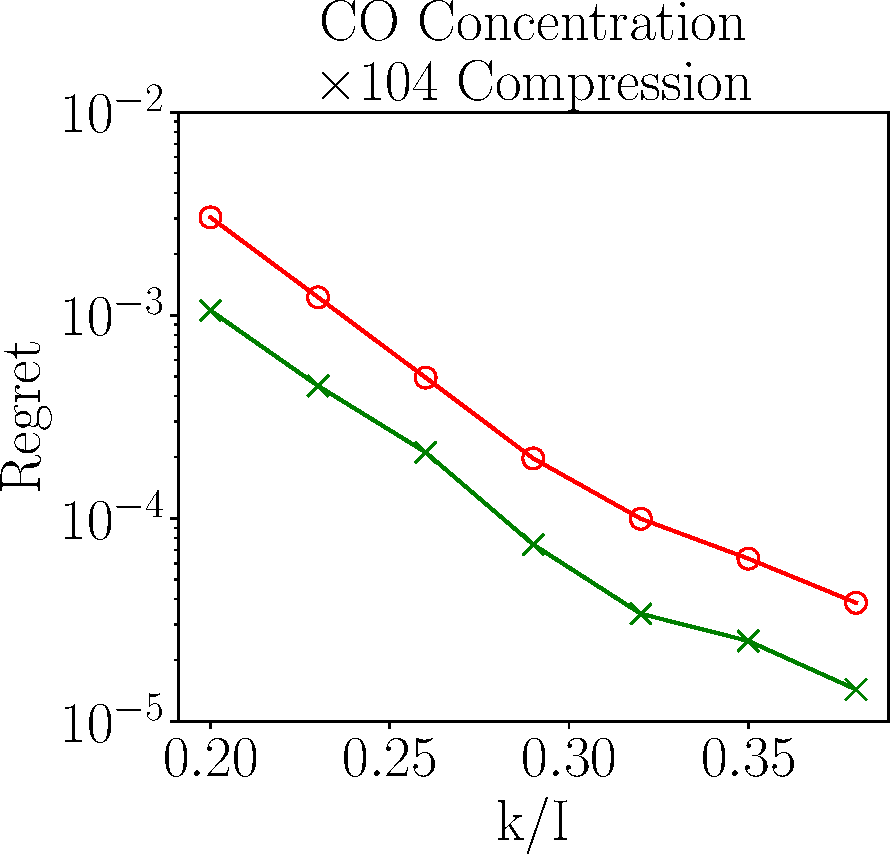
\includegraphics[height=2.9cm]{figure/multi_CO_frk10.pdf}
	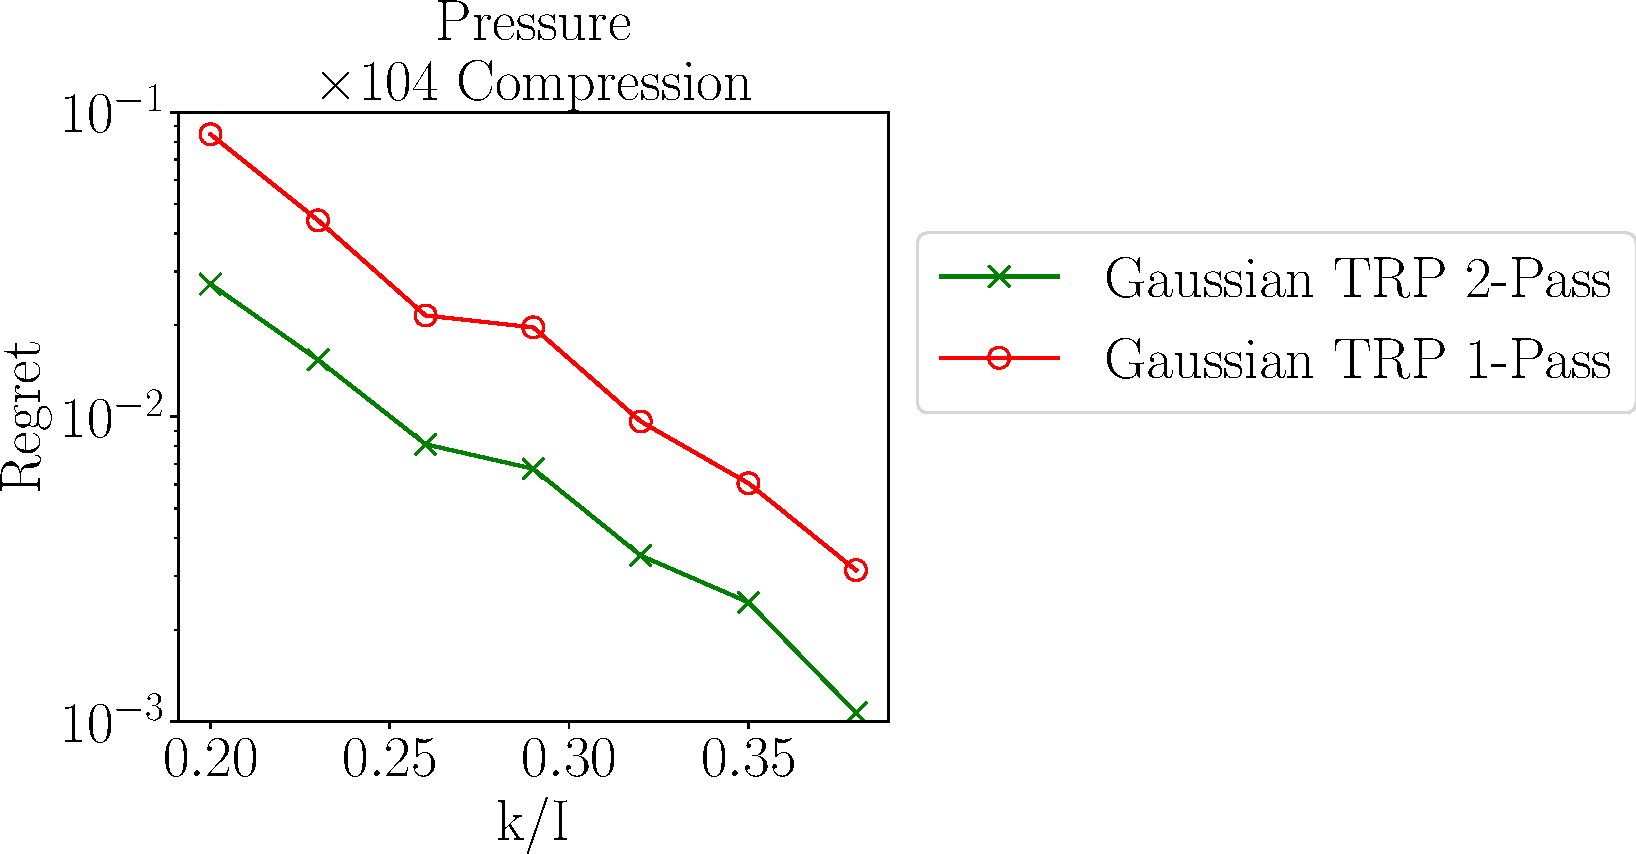
\includegraphics[height=2.9cm]{figure/multi_P_frk10.pdf}\\
	\textbf{Combustion Simulation}\\
	\caption{\textit{Approximations improves with more memory: real data.}
		% The aerosol absorption data	($240 \times 30 \times 192 \times 288$) is from CESM CAM 5.0.
		% The combustion data %for pressure, CO concentration, and temperature
		% (all of size $1408 \times 128 \times 128$)
		% is from \cite{lapointe2015differential}.
		We approximate aerosol absorption and combustion data
		using our one-pass and two-pass algorithms with the Gaussian TRP.
		We compare three target ranks ($r/I = 0.125,0.1,0.067$) for the former,
		and use the same target rank ($r/I = 0.1$) for each measured quantity in
		the combustion dataset.
		Notice $r/I = 0.1$ gives a hundred-fold compression!
	}\label{fig:climate}
\end{figure}

\begin{figure}[h!]
	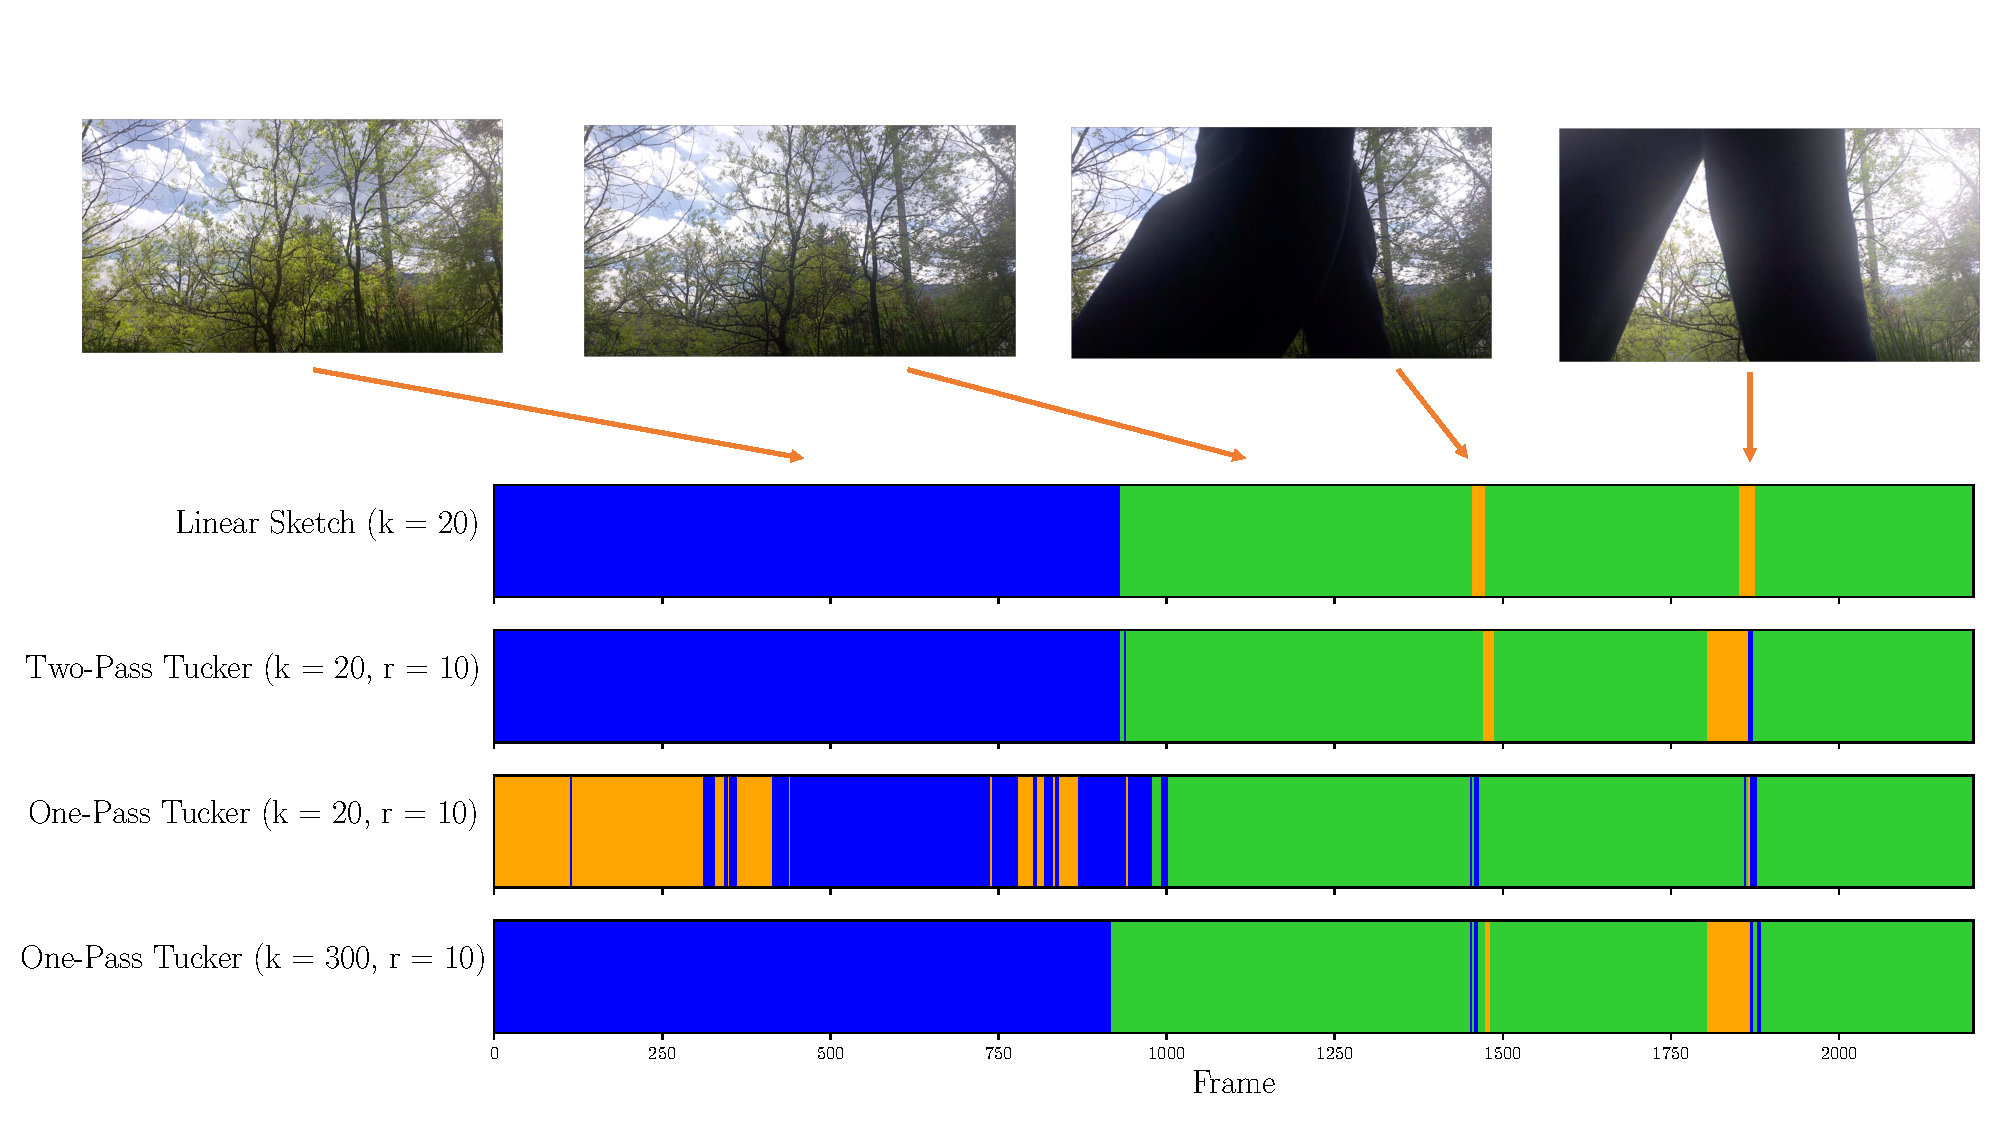
\includegraphics[height=7cm]{figure/video_classification_result.pdf} \\
	\centering
	\textbf{Video Scene Classification}
	\caption{\textit{Video Scene Classification}
		($2200 \times 1080 \times 1980$):
		We classify frames from the video data
		from \cite{malik2018low} (collected as a third order tensor with size $2200 \times 1080 \times 1980$) using $K$-means with $K$=3 on vectors computed using four different methods. $s = 2k+1$ throughout.
		1) The linear sketch along the time dimension (Row 1).
		2-3) the Tucker factor along the time dimension,
		computed via our two-pass (Row 2) and one-pass (Row 3) algorithms.
		%with parameters $r=10$, $k = 20$, and $s = 41$.
		4) The Tucker factor along the time dimension,
		computed via our one-pass (Row 4) algorithm
		%with parameters $r=10$, $k = 300$, and $s = 601$.
		}\label{fig:video}
\end{figure}

\begin{figure}[h!]
	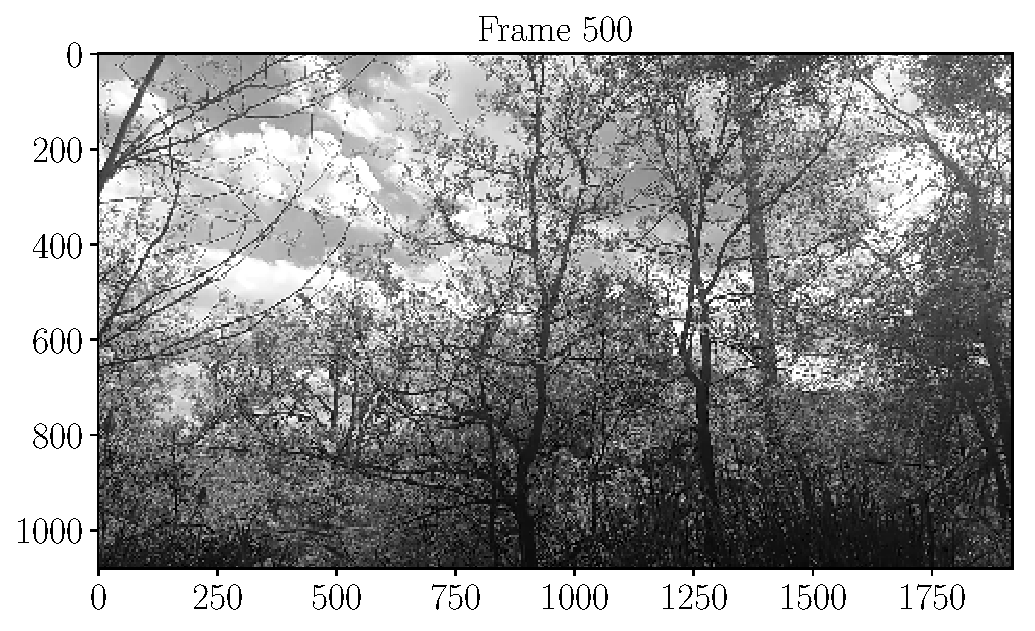
\includegraphics[height=2.4cm]{figure/frame500.pdf}
	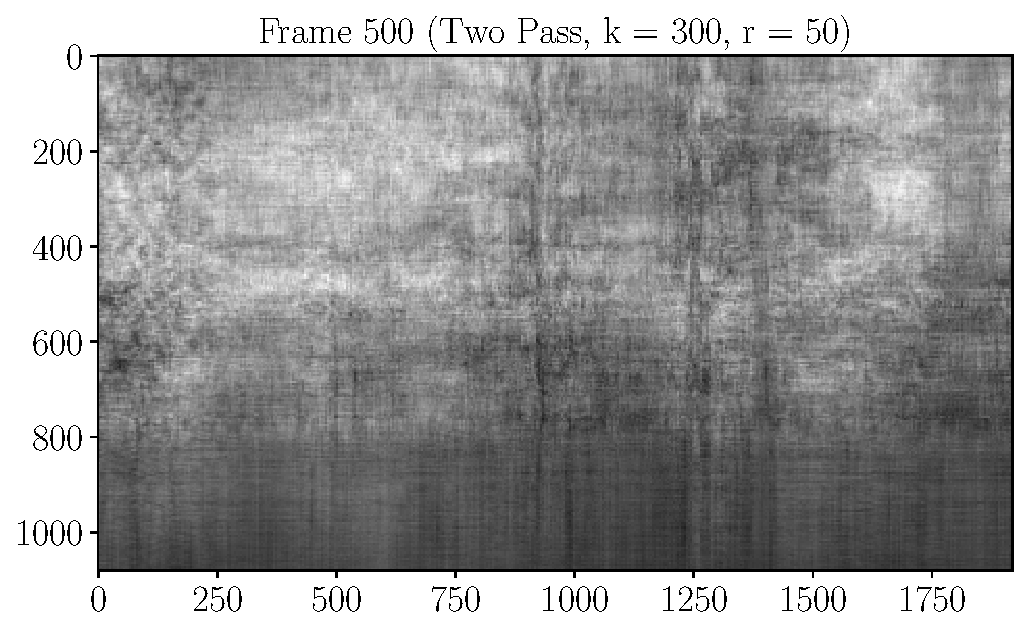
\includegraphics[height=2.4cm]{figure/2pass_k300_r50_frame500.pdf}
	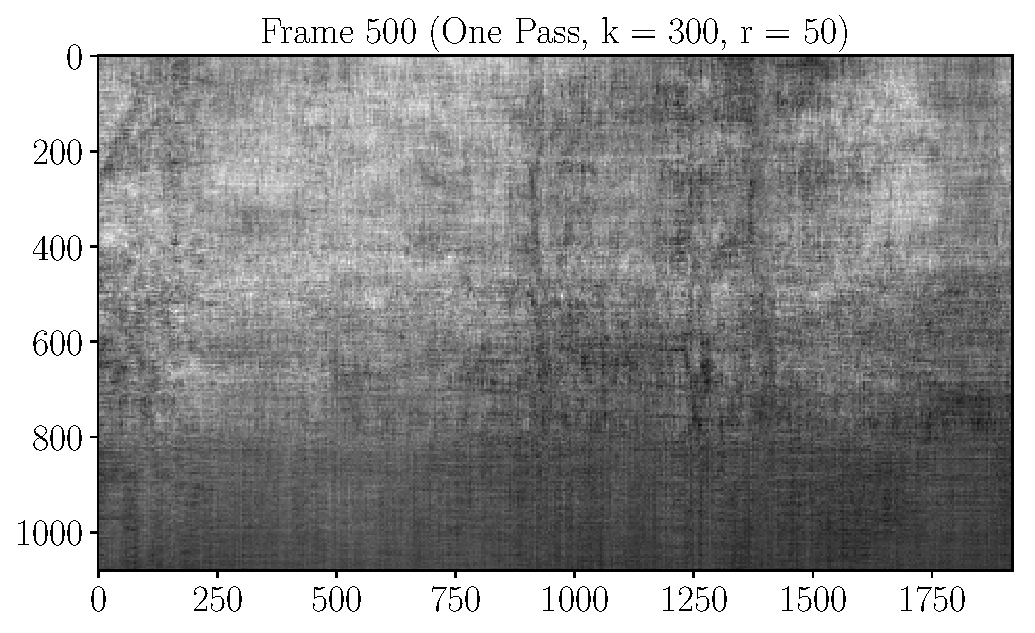
\includegraphics[height=2.4cm]{figure/1pass_k300_r50_frame500.pdf}
	\centering
	\caption{\textit{Visualizing Video Recovery:}
	Original frame (left);
	approximation by two-pass sketch (middle);
	approximation by one-pass sketch (right).
	% Frame 500
	}\label{fig:Frame500}
\end{figure}

\begin{figure}[h!]
	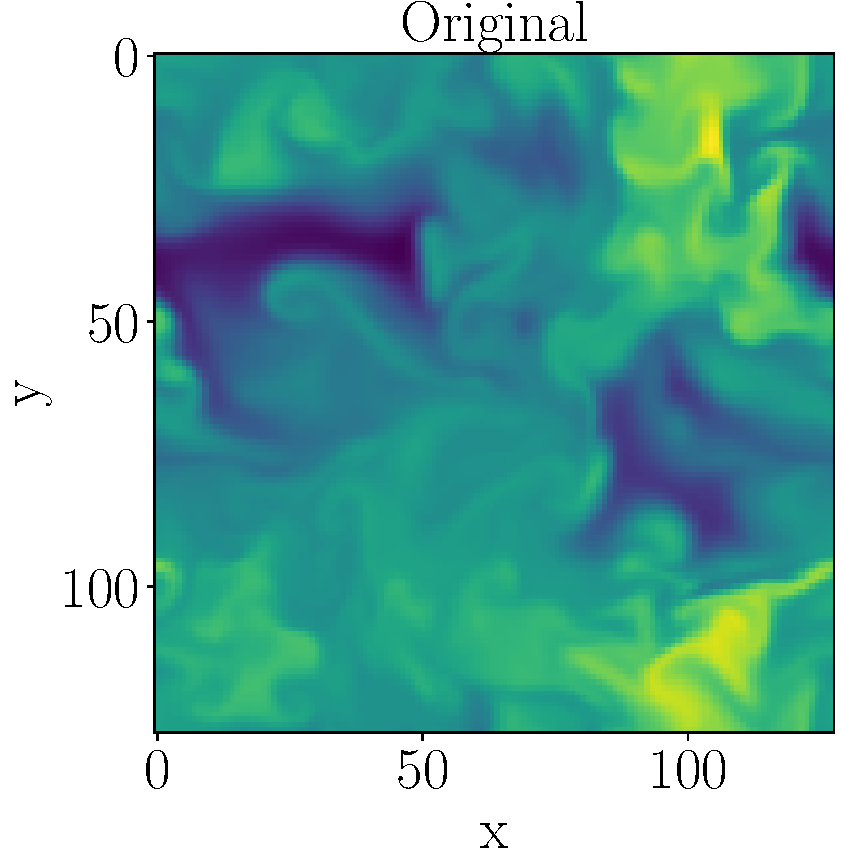
\includegraphics[height=3cm]{figure/T100_original.pdf}
	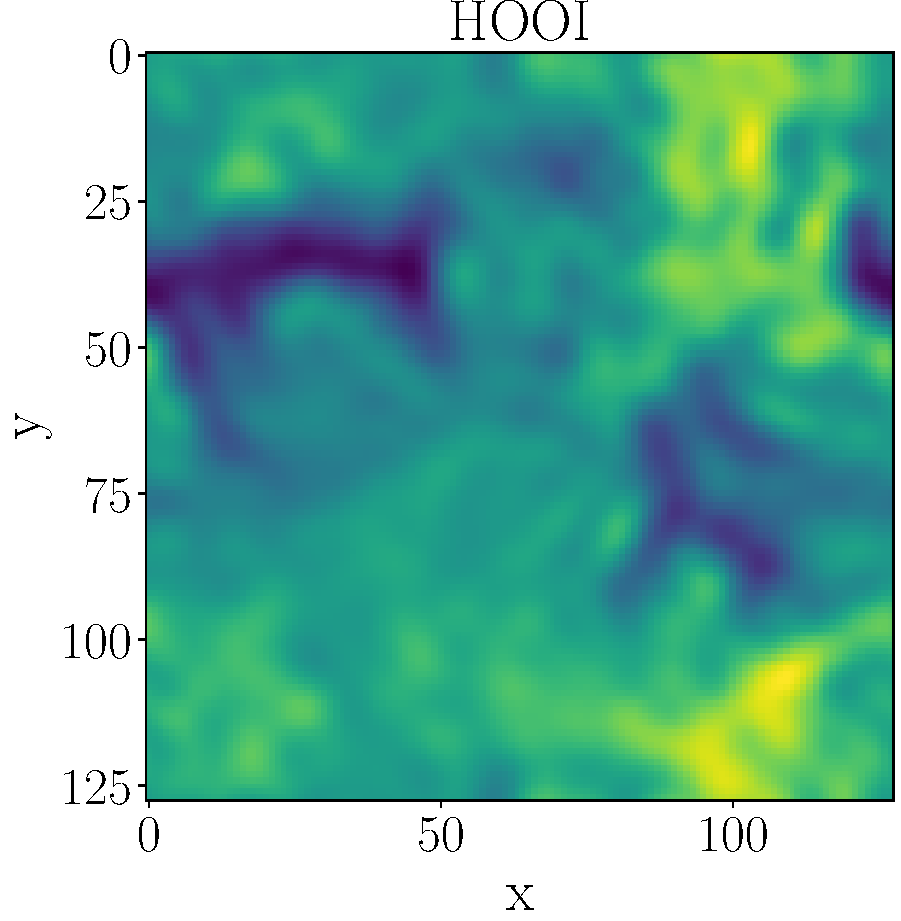
\includegraphics[height=3cm]{figure/T100_hooi.pdf}
	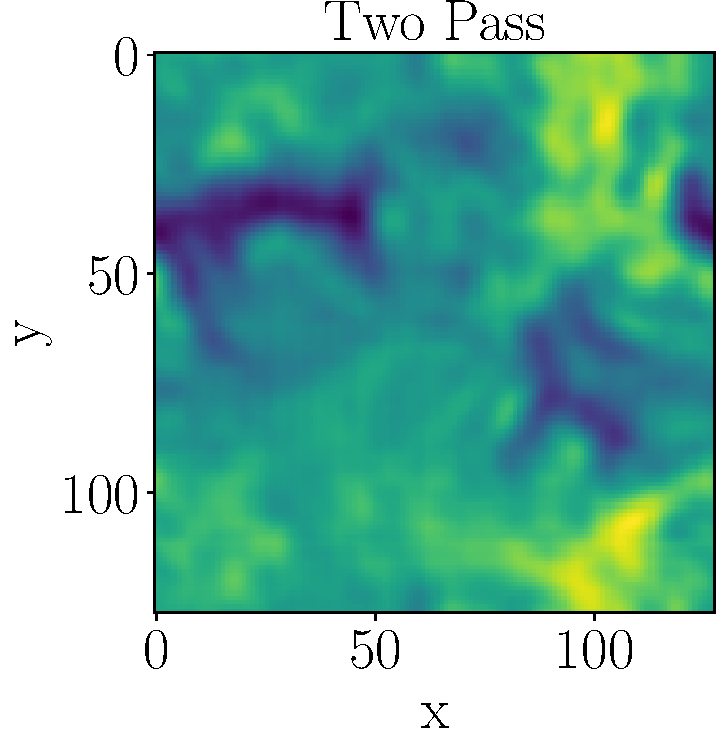
\includegraphics[height=3cm]{figure/T100_2pass.pdf}
	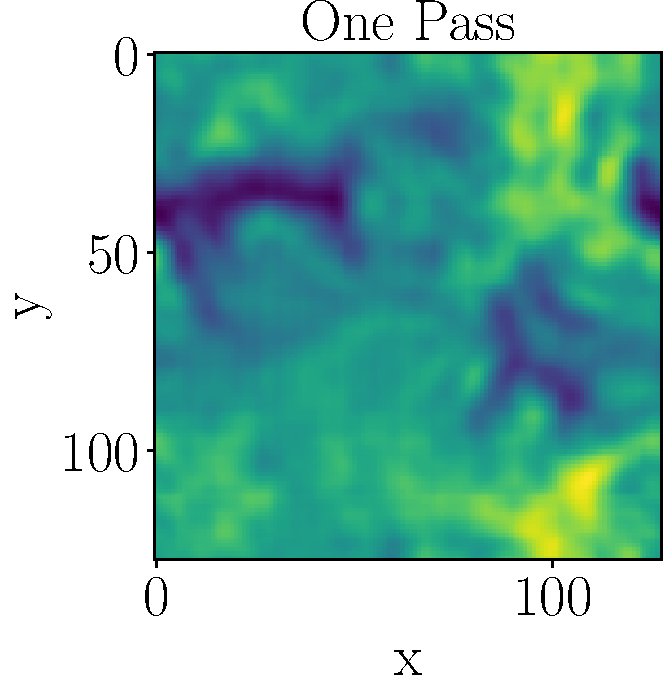
\includegraphics[height=3cm]{figure/T100_1pass.pdf}
	\centering
	\caption{\label{fig:T100}\textit{Visualizing Combustion Simulation:}
	All four figures show a slice of the temperature data along the first dimension.
	The approximation uses
	$\mathbf{r} = (281,25,25)$,
	$\mathbf{k} = (562,50,50)$,
	$\mathbf{s} = (1125, 101, 101)$,
	with the Gaussian TRP in the Tucker sketch.}
\end{figure}

\subsubsection{A second pass reduces error}
The second experiment compares our two-pass and one-pass algorithm.
The design is similar to the first experiment.
\ref{fig:vary-k-600-compare} shows that the two-pass algorithm
typically outperforms the one-pass algorithm,
especially in the high-noise, sparse, or rank-decay case.
Both converge at the same asymptotic rate.
(Results for other input tensors are available
\ifdefined \issupplement
in the supplement.)
\else
%in \ref{fig:vary-k-400-compare-app} and \ref{fig:vary-k-200-compare-app}
in \ref{appendix:more_result}.)
\fi

\subsubsection{Improvement on state-of-the-art}
The third experiment compares the performance of our two-pass and one-pass algorithms
and Tucker TensorSketch (T.--TS), as described in \cite{malik2018low},
the only extant one-pass algorithm.
For a fair comparison, we allocate the same storage budget to each algorithm
and compare the relative error of the resulting fixed-rank approximations.
We approximate synthetic 3D tensors with side length $I = 300$
with Tucker rank $r = 10$.
We use the suggested parameter settings for each algorithm:
$k = 2r$ and $s =2k+1$ for our methods; $K = 10$ for T.--TS.
Our one-pass algorithm
(with the Gaussian TRP)
uses $((2k+1)^N + kIN)$ storage,
whereas T.-TS uses $(Kr^{2N}+Kr^{2N-2})$ storage
\ifdefined \issupplement
(see supplement).
\else
(see \ref{tab:storage-comparison} in \ref{appendix: time-complexity}).
\fi

% Specifically, we choose $k$ linear in log scale within $\in [12,115]$,
% corresponding to $K \in [0.026,12]$ in \cite{malik2018low} \ref{fig:vary-memory}.

Figure \ref{fig:vary-memory} shows that our algorithms generally perform as well as T.--TS,
and dramatically outperforms for small storage budgets.
%two-pass algorithm always outperforms our one-pass algorithm, by a modest margin.
For example, our method achieves 1/50, 1/50, 1/7, and 1/4 the relative error of T.--TS
for low rank and sparse low rank ($\gamma = 0.01$), low rank ($\gamma = 0.1$), and polynomial-decay
input tensors, respectively.
For the low rank ($\gamma = 1$) tensor, the performance of T.--TS is not even monotone as the storage budget increases!
% In the case when the design tensor has a rank decay along its super diagonal, our algorithm is able to easily recover the low-rank signal, while their method is highly unstable and likely to give a worse result even in their suggested setting.
The performance of T.--TS is comparable with that of
the algorithms presented in this paper only when the storage budget is large.
%In both the low-rank and sparse low-rank settings, their method outperforms our method for very large memory usage.

\begin{remark}
	The paper \cite{malik2018low} proposes a multi-pass method, Tucker Tensor-Times-Matrix-TensorSketch (TTMTS) that is dominated by the one-pass method Tucker TensorSketch(TS) in all numerical experiments;
  hence we compare only with T.-TS.
\end{remark}

\subsection{Applications}\label{s-real-data}

We also apply our method to datasets drawn from three application domains:
climate, combustion, and video.
\begin{itemize}
\item \emph{Climate data.}
We consider global climate simulation datasets from
the Community Earth System Model (CESM) Community Atmosphere Model (CAM) 5.0 \cite{hurrell2013community,kay2015community}.
The dataset on aerosol absorption has four dimensions:
times, altitudes, longitudes, and latitudes  ($240 \times 30 \times 192 \times 288$).
% show in appendix
The data on net radiative flux at surface and dust aerosol burden have three dimensions:
times, longitudes, and latitudes ($1200 \times 192 \times 288$).
Each of these quantitives has a strong impact on the absorption of solar radiation and on cloud formation.

\item \emph{Combustion data.}
We consider combustion simulation data from \cite{lapointe2015differential}.
% This paper aims to understand the effect of differential diffusion, distributed burning,
% and local distinction under different circumstances.
The data consists of three measured quantities ---
pressure, CO concentration, and temperature ---
each observed on a $1408 \times 128 \times 128$ spatial grid.
% At each time, we choose three measured quantities out of the 40 measured quantities (all of size $1408 \times 128 \times 128$) at different locations to compress, specifically the pressure, CO concentration, and temperature.

\item \emph{Video data.}
We use our streaming method to cluster frames of a video,
as in \cite{malik2018low}.
Here, a low frame rate camera is mounted in a fixed position as people walk by.
A 3D tensor is constructed with each video frames as a slice.
%The rank of the tensor corresponds to the number of people seen. (The background is rank 2.)
The video consists of 2493 frames, each of size 1080 by 1980.
%  in grayscale,
% thus of size (2493 $\times$ 1080 $\times$ 1980).
As a tensor, stored as a \texttt{numpy.array}, the video data is 41.4 GB in total.
\end{itemize}

\subsubsection{Data compression}
We show that our proposed algorithms are able to
successfully compress climate and combustion data
even when the full data does not fit in memory.
%, we want to compress the huge original tensor into a low-rank Tucker decomposition efficiently.
Since the Tucker rank of the original tensor is unknown, we perform experiments for
three different target ranks. In this experiment, we hope to understand the effect of different choices of storage budget $k$ to
 achieve the same compression ratio. We define the compression ratio
 as the ratio in size between the original input tensor and the output Tucker factors, i.e. $\frac{\prod_{i = 1}^N I_i}{\sum_{i=1}^Nr_iI_i+ \prod_{i = 1}^N r_i}$.
As in our experiments on simulated data, \ref{fig:climate} shows
that the two-pass algorithm outperforms the one-pass algorithm as expected.
However, as the storage budget $k$ increases, both methods converge to the performance of HOOI.
The rate of convergence is faster for smaller target ranks.
Performance of our algorithms on the combustion simulation is qualitatively similar,
but converges faster to the performance of HOOI. \ref{fig:T100} visualizes the recovery of
the temperature data in combustion simulation for a slice along the first dimension. We could observe that the
recovery for both two-pass and one-pass algorithm approximate the recovery from HOOI.
% Indeed, but in general with a faster convergence rate than the climate data even when the data is not perfectly low rank, like the pressure data.
\ifdefined \issupplement
Similar results on other datasets appear in the supplement.)
\else
\ref{fig:srfrad_burden_dust} in \ref{appendix:more_real_data_result}
shows similar results on another dataset.
\fi

\subsubsection{Video scene classification}
We show how to use our single pass method to classify scenes in the video data described above.
The goal is to identify frames in which people appear.
% In our experiment, we split the dataset into nine segments each of size $277 \times 1080 \times 1980$.
% \mnote{why split?}
We remove the first 100 frames and last 193 frames where the camera setup happened,
as in \cite{malik2018low}.
We stream over the tensor and sketch it using parameters $k = 300, s = 601$.
Finally, we compute a fixed-rank approximation with $\mathbf{r} = (10,10,10)$ and $(20,20,20)$.
We apply K-means clustering to the resulting 10 or 20 dimensional vectors
corresponding to each of the remaining 2200 frames.

We experimented with clustering vectors found in three ways:
from the two-pass or one-pass Tucker approximation,
or directly from the factor sketch. % without performing the reconstruction.

When matching the video frames with the classification result,
we can see that the background light is relatively dark at the beginning,
thus classified into \texttt{Class} $0$.
After a change in the backgroun light,
most other frames of the video are classified into \texttt{Class} $1$.
When a person passes by the camera, the frames are classified into \texttt{Class} $2$.
Right after the person passed by, the frames are classified into \texttt{Class} $0$,
the brighter background scene, due to the light adjustment.

Our classification results (using the linear sketch or approximation)
are similar to those in \cite{malik2018low}
while using only $1/500$ as much storage; the one pass approximation
requires more storage (but still less than \cite{malik2018low}) 
to achieve similar performance.
In particular, using the sketch itself, rather than the Tucker approximation,
to summarize the data enables very efficient video scene classification.

On the other hand, to reconstruct the original video frames
we require much larger $\mathbf{k}$ and $\mathbf{r}$:
the video is not very low rank along the spatial dimensions.
\ref{fig:Frame500} shows that
even with $\mathbf{s} = {601, 601, 601}, \mathbf{k} = (300, 300, 300), \mathbf{r} = (50, 50, 50)$, the recovered frame is very noisy.
% The memory and computational requirements of HOOI exceed our capacity,
% so we cannot apply it to the video data.

% \section*{Conlusion}
We propose to do adaptive thresholding for weakly sparse spectral density estimation. In order to conquer some technical difficulty, we propose a new modified periodogram, which has the same  order in bias compared to the classic periodogram, while provides great convenience in theoretical development. Our adaptive thresholding relax the constraint in maximum operator norm  and achieve better convergence rate in theory. 
\section*{Acknowledgments}
MU, YS, and YG were supported in part by DARPA Award FA8750-17-2-0101.
JAT gratefully acknowledges support from ONR Awards N00014-11-10025, N00014-17-12146, and N00014-18-12363.
The authors wish to thank Osman Asif Malik and Stephen Becker for their help
in understanding and implementing Tucker TensorSketch,
and Tamara Kolda for insightful comments on an early draft.

% bibliography
\clearpage
\bibliographystyle{siamplain}
\bibliography{bibtex}

\appendix
\begin{appendices}
\onecolumn
% proofs
\section{Proof of Main Results}
\label{appendix:proof-main-result}
% To bound the approximation error of the algorithms presented in the main body
% of this paper, we first develop several structural results showing
% an additive decomposition of the error.
% First, the total error is the sum of the error due to sketching
% and the error due to fixed rank approximation.
% Second, the sketching error is the sum of the error due to the factor matrix
% approximations and to the core approximation.
% Third, the error due to the factor matrix approximations
% is the sum of the error in each the modes,
% as the errors due to each mode are mutually orthogonal.
% This finishes the approximation error bound for the two pass algorithm, \ref{thm:low_rank_err_two_pass}.
% As for the error due to the core approximation,
% we give a combinatorial argument to rewrite the approximation error in the core tensor
% as a sum over each mode of errors that are mutually orthogonal.
% Indeed, these errors have the same form as the errors due to the factor matrix approximations,
% scaled down by a factor $\Delta(k,s)$ that depends on the sketch sizes $\V{k}$ and $\V{s}$.
% This argument shows the error due to the core approximation
% is at most a factor $\Delta(k,s)$ times the error due to the factor matrix approximation.

% Yiming wrote:
% For low rank approximation, since there is no any optimization procedure involved, all the errors come from sketching stage. For fixed rank approximation, we also need to take the recovery error (from Tucker decomposition)  into consideration. But for tensor decomposition, the approximation error is impossible to be described as clear as that in matrix case(singular value decomposition). we include the best approximation error in our result. Essentially for both case, our theory focuses in building statistical  error bound introduced by the sketching and leave the recovery error in terms of the best approximation error: $\|\T{X} - \llbracket \T{X} \rrbracket_\mathbf{r}\|_F$.
%
% For sketching stage, we consider errors introduced by arm sketch and core sketch
% respectively. Arm sketch essentially is a series of projection of original tensor to column space the sketch corresponding along each mode. We demonstrate that we can decompose the error as sum of errors along each mode by showing they are orthogonal to each other. For the error from core sketch, by some combinatoric argument, we essentially treat the approximation error for core tensor as $\sum_n \rm{Approx}(\T{Z}_n)$ where $\sum_n \T{Z}_n = \T{X} - \T{\hat{X}}$, $\langle \T{Z}_m, \T{Z}_n \rangle = 0$ and $\rm{Approx}(\T{Z}_n)$ is some approximation of $\T{Z}_n$ satisfying $\|\rm{Approx}(\T{Z}_n) -\T{Z}_n\|_F \le \Delta(k,s) \|\T{Z}_n\|_F$ where $\Delta(k,s)$ is a constant depending in sketch size $k,s$. This essentially claims that the error from core sketch is at most $\Delta(k,s)$ of error from arm sketch.

\subsection{Error bound for the two pass approximation Algorithm \ref{alg:two_pass_low_rank_appro}}
\begin{proof}[Proof of Theorem \ref{thm:low_rank_err_two_pass}]
Suppose $\T{\hat{X}}_2$ is the low-rank approximation from \ref{alg:two_pass_low_rank_appro}.
Use the definition of the mode-$n$ product to see
\begin{equation*}
\begin{aligned}
\T{\hat{X}}_2 &=  \left[\T{X}\times_1 \mathbf{Q}_1^\top \times_2 \cdots \times_N \mathbf{Q}_N^\top\right] \times_1 \mathbf{Q}_1\times_1 \cdots\times_N \mathbf{Q}_N\\
&= \T{X}\times_1 \mathbf{Q}_1\mathbf{Q}_1^\top \times_2 \cdots \times_N \mathbf{Q}_N\mathbf{Q}_N^\top.
\end{aligned}
\end{equation*}
Although it seems that we sequentially project tensor $\T{X}$ to column space spanned with $\mathbf{Q}_n$, but since mode product is exchangeable, in fact $\hat{\T{X}}_2$ is the projection to space $\{ \T{X} : \T{X}^{(n)} 
\in \mathbf{col}(\mathbf{Q}_n) \}$.  This is a generalization of projection matrix where \cite{de2008tensor} has a very detailed  explanation and it is referred as multi-linear orthogonal projection.  Following exact techniques in Theorem 5.1 in \cite{vannieuwenhoven2012new} by sequentially applying Pythagorean theory sequentially we can show that 
\begin{equation}
\|\hat{\T{X}}_2 - \T{X}\|_F^2 \le \sum_{n=1}^N  \left \| (\mathbf{I} - \mathbf{Q}_n\mathbf{Q}_n^\top) \mathbf{X}^{(n)} \right\|_F^2 .
\end{equation}
Then taking expectation on $\mathbf{Q}_n$, and applying Lemma \ref{lemma:sketchy_column_space_err} we complete the proof. 




\end{proof}

\subsection{Error bound for the one pass approximation Algorithm \ref{alg:one_pass_low_rank_appro}}
\begin{proof}[Proof of Theorem \ref{thm:low_rank_err}]
We show the approximation error can be decomposed as
the error due to the factor matrix approximations
and the error due to the core approximation.
Let $\T{\hat{X}}_1$ be the one pass approximation from \ref{alg:one_pass_low_rank_appro}, and let
\begin{equation}
\T{\hat{X}}_2 = \T{X}\times_1 \mathbf{Q}_1\mathbf{Q}_1^\top \times_2 \cdots \times_N \mathbf{Q}_N\mathbf{Q}_N^\top,
\end{equation}
be the two pass approximation from \ref{alg:two_pass_low_rank_appro}.
The difference in one-pass and two-pass approximation is in the 
core: 
\begin{equation}
\begin{aligned}
\T{\hat{X}}_1-\hat{\T{X}}_2= (\T{W}-\T{X}\times_1 \mathbf{Q}_1^\top \times_2 \cdots \times_N \mathbf{Q}_n^\top)  \times_1 \mathbf{Q}_1 \dots \times_N \mathbf{Q}_N. \nonumber
\end{aligned}
\end{equation}
Thus $\T{\hat{X}}_1-\hat{\T{X}}_2$ is in the space defined above:  $\{ \T{X} : \T{X}^{(n)} 
\in \mathbf{col}(\mathbf{Q}_n) \}$ while as pointed before $\hat{\T{X}}_2 - \T{X}$ is perpendicular  to that space.  Therefore, 

\begin{equation}
\label{eq:inner_zero}
\langle \hat{\T{X}}_1 - \hat{\T{X}}_2, \hat{\T{X}}_2 - \T{X} \rangle = 0.
\end{equation}


Now we use the (expectation of) the Pythagorean theorem 
to bound the expected error of the one pass approximation:
\begin{equation}
\label{eq:error_decom}
 \mathbb{E}\| \hat{\T{X}}_1- \T{X} \|_F^2 = \mathbb{E}\| \hat{\T{X}}_1 - \hat{\T{X}}_2\|_F^2 + \mathbb{E} \|\hat{\T{X}}_2 - \T{X} \|_F^2.
\end{equation}



Consider the first term which is due to core approximation. Based in the definition of $\hat{\T{X}}_1$ and $\tilde{\T{X}}_2$ we can see that 
\begin{align*}
\|\hat{\T{X}}_1 - \hat{\T{X}}_2\|^2_F &=
\|(\T{W}_1 - \T{X}\times_1 \mathbf{Q}_1^\top \cdots \times_N \mathbf{Q}^\top_N)\times_1 \mathbf{Q}_1\cdots \times_N \mathbf{Q}_N \|^2_F\\
& = \|(\T{W}_1- \T{X}\times_1 \mathbf{Q}_1^\top \cdots \times_N \mathbf{Q}^\top_N)\|_F^2,
\end{align*}
where we use the invariance of the Frobenius norm under orthonormal transformations to get the second line.
Now using \ref{lemma:err_core_sketch} to bound for the error due to the core approximation as
%(the first term in \eqref{eq:error_decom}) as
\begin{equation}
\mathbb{E} \|\hat{\T{X}}_1- \hat{\T{X}}_2\|^2_F \le \Delta \left[ \sum_{n=1}^N \left(1+\frac{\rho_n}{k_n-\rho_n-1}\right)(\tau^{(n)}_{\rho_n})^2\right].\nonumber
\end{equation}

Finally, as shown in proof for  \ref{thm:low_rank_err_two_pass} to
bound the error due to the factor matrix approximations
(the second term in \eqref{eq:error_decom}) as
\begin{equation}
\mathbb{E}\|\hat{\T{X}}_2 - \T{X} \|_F^2 \le \left[ \sum_{n=1}^N \left(1+\frac{\rho_n}{k_n-\rho_n-1}\right)(\tau^{(n)}_{\rho_n})^2\right].\nonumber
\end{equation}
Summing these two bounds finishes the proof.
\end{proof}

\subsection{Error bound for the fixed rank approximation Algorithm  \ref{alg:one_pass_fix_rank_appro}}

\begin{proof}[Proof of Theorem \ref{thm:fix_rank_err}]
Our argument follows the proof of \cite[Proposition 6.1]{tropp2017practical}:
\begin{equation}
\begin{aligned}
&\|\T{X} - \llbracket \hat{\T{X}} \rrbracket_\mathbf{r}\|_F \le \|\T{X} -  \hat{\T{X}}\|_F+\|\hat{\T{X}} -  \llbracket\hat{\T{X}}\rrbracket_\mathbf{r}\|_F\\
&\le \|\T{X} -  \hat{\T{X}}\|_F+\|\hat{\T{X}} -  \llbracket \T{X}\rrbracket_\mathbf{r}\|_F \\
& \le \|\T{X} -  \hat{\T{X}}\|_F+\|\hat{\T{X}} - \T{X}  + \T{X} - \llbracket \T{X}\rrbracket_\mathbf{r}\|_F \\
&\le 2\|\T{X} - \hat{\T{X}} \|_F + \|\T{X} -  \llbracket \T{X} \rrbracket_\mathbf{r}\|_F.\nonumber
\end{aligned}
\end{equation}
The first and the third line are the triangle inequality,
and the second line follows from the definition of the best rank-$r$ approximation.
Take the expectation of $\|\T{X} - \hat{\T{X}} \|_F$ and
use Jensen's inequality $\mathbb{E}\|\T{X} - \hat{\T{X}} \|_F \le \sqrt{\mathbb{E} \|\T{X} - \hat{\T{X}} \|_F^2}$
to finish the proof.
\end{proof}

%\section{Probabilistic Analysis of the Compression Error}

\begin{lem}
\label{lemma: compression_error}
For any natural numbers $\rho_n$, $1\le \rho_n<k_n-1$,
\begin{equation}
\mathbb{E}  \|\tilde{\T{X}} - \T{X}\|_F^2 \le \sum_{n=1}^N \left(1+\frac{\rho_n}{k-\rho_n-1}\right)(\tau^{(n)}_{\rho_n})^2,\nonumber
\end{equation}
where $\tilde{\T{X}}$ is the two pass approximation defined in \eqref{eq:x_tilde}.
\begin{proof}
This proof extends the result for matrix sketching stated in \cite{halko2011finding} to the tensor case.
To construct a similar bound, we first decompose the square norm of the compression error
into the sum of square norms of the differences $\T{Y}_{n-1} - \T{Y}_{n}$ in \eqref{eq: y_diff},
and then bound each term individually in \eqref{eq: y_diff_bound}.
Again, we will show that the inner products between these differences are always zero.

Following the definition of $\T{Y}_n$ in \ref{eq:definition_Y_n},
\begin{equation}\label{eq: y_diff}
\begin{aligned}
& \|\T{X}-\tilde{\T{X}}\|_F^2 = \|\T{Y}_0 - \T{Y}_N\|_F^2= \left\|\sum_{n=0}^{N-1} (\T{Y}_n - \T{Y}_{n+1})\right\|_F^2.
\end{aligned}
\end{equation}
For any $0 \leq m \leq N-1$,
\begin{equation}
\T{Y}_m-\T{Y}_{m+1} = \T{Y}_{m} \times_{(m+1)} (\mathbf{I} - \mathbf{Q}_{m+1}\mathbf{Q}^\top_{m+1}). \nonumber
\end{equation}
and for any $0\le m< n < N$, define $\T{A}^{(m,n)}$ using the equation
$\T{Y}_n - \T{Y}_{n+1} =$
\begin{multline}
\underbrace{\left[\T{X}\times_1 \mathbf{Q}_{1}\mathbf{Q}^\top_{1} \times_2 \cdots \times_{m} \mathbf{Q}_{m}\mathbf{Q}^\top_{m}\times_{(m+2)} \cdots  \times_{n} \mathbf{Q}_{n}\mathbf{Q}^\top_{n}\times_{(n+1)}(\mathbf{I}-\mathbf{Q}_{(n+1)}\mathbf{Q}^\top_{(n+1)})\right]}_{\T{A}}\\
	\times_{(m+1)} \mathbf{Q}_{m+1}\mathbf{Q}^\top_{m+1}.\nonumber
\end{multline}
The second part of \ref{lemma:projection_tensors} shows
\begin{equation}\label{eq:inner_prod1}
\langle\T{Y}_m-\T{Y}_{m+1},  \T{Y}_n - \T{Y}_{n+1}\rangle = \langle\T{Y}_{m} \times_{(m+1)} (\mathbf{I} - \mathbf{Q}_{m+1}\mathbf{Q}^\top_{m+1}), \T{A}^{(m,n)} \times_{m+1} \mathbf{Q}_{m+1}\mathbf{Q}^\top_{m+1} \rangle = 0.\nonumber
\end{equation}
Hence we can decompose the error in the two pass approximation as
\begin{equation}
\label{eq:comression_decomposition}
\begin{aligned}
& \|\T{X}-\tilde{\T{X}}\|_F^2 =  \sum_{n=0}^{N-1} \| (\T{Y}_n - \T{Y}_{n+1})\|_F^2
\end{aligned}
\end{equation}
by the Pythagorean theorem.
Now we bound $\|\T{Y}_n - \T{Y}_{n+1}\|_F^2$ for each $n$:
\begin{equation} \label{eq: y_diff_bound}
\begin{aligned}
\|\T{Y}_n - \T{Y}_{n+1}\|_F^2 &= \|\T{X}\times_{(n+1)} (\mathbf{I} - \mathbf{Q}_{n+1}\mathbf{Q}_{n+1}^\top)\times_{1} \mathbf{Q}_{1}\mathbf{Q}_{1}^\top\dots \times_n \mathbf{Q}_{n}\mathbf{Q}_{n}^\top\|_F^2 \\
&\le \|\T{X}\times_{(n+1)} (\mathbf{I} - \mathbf{Q}_{n+1}\mathbf{Q}_{n+1}^\top)\|_F^2 \\
&= \| (\mathbf{I} - \mathbf{Q}_{n+1}\mathbf{Q}_{n+1}^\top)\mathbf{X}^{(n)}\|_F^2,
\end{aligned}
\end{equation}
where the second line follows from the fact that the projection is contractive,
together with second part of \ref{lemma:projection_tensors}.
Apply \ref{lemma:sketchy_column_space_err} to the last line of the inequality above to show
\begin{equation}
\mathbb{E} \|\T{Y}_n - \T{Y}_{n+1}\|_F^2 \le \left(1+\frac{\rho_n}{k_n-\rho_n-1}\right)(\tau^{(n+1)}_{\rho_n})^2.\nonumber
\end{equation}
Sum the bound for each term in  \eqref{eq:comression_decomposition} to finish the proof.
\end{proof}
\end{lem}

\section{Probabilistic Analysis of Core Sketch Error}
This section contains the most technical part of our proof.
We provide a probabilistic error bound for the difference between the
two pass core approximation $\T{W}_2$
from Algorithm \ref{alg:two_pass_low_rank_appro}
and the one pass core approximation $\T{W}_1$
from Algorithm \ref{alg:one_pass_low_rank_appro}.
% We first prove that this error
% will show how to decompose this error first, and
% then take the expectation to obtain the probabilistic error bound.

Introduce for each $n\in[N]$ the orthonormal matrix $\M{Q}_n^\bot$ that forms
a basis for the subspace orthogonal to $\M{Q}_n$, so that
$\M{Q}_n^\bot (\M{Q}_n^\bot)^\top = \M{I} - \M{Q}_n\M{Q}_n^\top$.
Next, define
\begin{equation}
\label{eq: def-proj-Q}
\begin{aligned}
\M{\Phi}_n^Q = \M{\Phi}^\top_n \M{Q}_n  ,~~~~\M{\Phi}_n^{Q^\bot} = \M{\Phi}^\top_n \M{Q}_n^\bot.
\end{aligned}
\end{equation}
Recall that the DRMs $\M{\Phi}_n$ are i.i.d. Gaussian. Hence conditional on $\M{Q}_n$,
$\M{\Phi}_n^Q$ and $\M{\Phi}_n^{Q^\bot}$ are independent.

\subsection{Decomposition of Core Approximation Error}
In this section, we characterize the
difference between the one and two pass core approximations
$\T{W}_1-\T{W}_2 = \T{W}_1 - \T{X}\times_1 \M{Q}_1^\top \dots \times_N \M{Q}_N^\top$.
\begin{lem}
\label{lemma:core_error_decomposition}
Suppose that $\M{\Phi}_n$ has full column rank for each $n \in [N]$.
Then
\begin{equation}
\T{W}_1-\T{W}_2 = \T{W}_1 - \T{X}\times_1 \M{Q}_1^\top \dots \times_N \M{Q}_N^\top =
\sum_{(i_1,\dots, i_N) \in \{0,1\}^N, \sum_{j=1}^N i_j \geq 1} \T{Y}_{i_1\dots i_N}, \nonumber
\end{equation}
where
\begin{equation}
\label{eq:def_each_part}
\begin{aligned}
\T{Y}_{i_1\dots i_N} &= \T{X}\times_1 \left(\mathbf{1}_{i_1=0}\M{Q}_1^\top + \mathbf{1}_{i_1=1}(\M{\Phi}_1^{Q_1})^\dag  \M{\Phi}_1^{Q_1^\bot}(\M{Q}_1^\bot)^\top \right)\\
&\times_2 \cdots \times_N \left(\mathbf{1}_{i_N=0}\M{Q}_N^\top + \mathbf{1}_{i_1=1}(\M{\Phi}_N^{Q_N})^\dag  \M{\Phi}_N^{Q_N^\bot}(\M{Q}_N^\bot)^\top \right).
\end{aligned}
\end{equation}
\end{lem}
\begin{proof}
Let $\T{H}$ be the core sketch from \ref{alg:tensor_sketch}.
Write %the one pass core approximation
$\T{W}_1$ as
\begin{equation}
\begin{aligned}
\T{W}_1 &= \T{H}\times_1 (\M{\Phi}_1^\top \M{Q}_1)^\dag \times_2 \cdots \times_N (\M{\Phi}^\top_N \M{Q}_N)^\dag \\
&= (\T{X} -  \hat{\T{X}}_2)\times_1 \M{\Phi}^\top_1 \times_2 \cdots \times_N \M{\Phi}^\top_N  \times_1 (\M{\Phi}^\top_1 \M{Q}_1)^\dag \times_2 \cdots \times_N (\M{\Phi}^\top_N \M{Q}_N)^\dag
\\
&+ \hat{\T{X}}_2\times_1 \M{\Phi}^\top_1 \times_2 \cdots \times_N \M{\Phi}^\top_N \times_1 (\M{\Phi}^\top_1 \M{Q}_1)^\dag \times_2 \cdots \times_N (\M{\Phi}^\top_N \M{Q}_N)^\dag.\nonumber
\end{aligned}
\end{equation}
Using the fact that $(\M{\Phi}^\top_n \M{Q}_n)^\dag (\M{\Phi}^\top_n \M{Q}_n) =\M{I}$, we can simplify the second term as
\begin{equation}
\begin{aligned}
&\tilde{\T{X}}\times_1 \M{\Phi}^\top_1 \times_2 \cdots \times_N \M{\Phi}^\top_N \times_1 (\M{\Phi}^\top_1 \M{Q}_1)^\dag \times_2 \cdots \times_N (\M{\Phi}^\top_N \M{Q}_N)^\dag   \\
& = \T{X}\times_1 (\M{\Phi}^\top_1 \M{Q}_1)^\dag \M{\Phi}^\top_1\M{Q}_1\M{Q}_1^\top \times_2 \cdots \times_N (\M{\Phi}_N^\top \M{Q}_N)^\dag \M{\Phi}_N^\top\M{Q}_N\M{Q}_N^\top\\
& = \T{X}\times_1 \M{Q}_1^\top \times_2 \cdots \times_N \M{Q}_N^\top, \nonumber
\end{aligned}
\end{equation}
which is exactly the two pass core approximation $\T{W}_2$.
Therefore
\begin{equation}
\begin{aligned}
&\T{W}_1 -\T{W}_2= (\T{X} -  \tilde{\T{X}})\times_1 \M{\Phi}^\top_1 \times_2 \cdots \times_N \M{\Phi}^\top_N  \times_1 (\M{\Phi}^\top_1 \M{Q}_1)^\dag \times_2 \cdots \times_N (\M{\Phi}^\top_N \M{Q}_N)^\dag. \nonumber
\end{aligned}
\end{equation}
We continue to simplify this difference:
\begin{equation}
\begin{aligned}
(\T{X} -  \tilde{\T{X}})&\times_1 \M{\Phi}^\top_1 \times_2 \cdots \times_N \M{\Phi}^\top_N  \times_1 (\M{\Phi}^\top_1 \M{Q}_1)^\dag \times_2\cdots \times_N (\M{\Phi}^\top_N \M{Q}_N)^\dag \label{eq:core_err_decom} \\
& =(\T{X} -  \tilde{\T{X}})\times_1 (\M{\Phi}^\top_1\M{Q}_1)^\dag \M{\Phi}^\top_1 \times_2\cdots \times_N (\M{\Phi}^\top_N\M{Q}_N)^\dag \M{\Phi}_N^\top \\
& =  (\T{X} -  \tilde{\T{X}}) \times_1 (\M{\Phi}^\top_1\M{Q}_1)^\dag \M{\Phi}^\top_1(\M{Q}_1\M{Q}_1^\top + \M{Q}_1^\bot (\M{Q}_1^\bot)^\top)\dots  \\
& \times_N (\M{\Phi}^\top_N\M{Q}_N)^\dag \M{\Phi}^\top_N(\M{Q}_N\M{Q}_N^\top + \M{Q}_N^\bot (\M{Q}_N^\bot)^\top)\\
& = (\T{X} -  \tilde{\T{X}}) \times_1 (\M{Q}_1^\top + (\M{\Phi}_1^Q)^\dag  \M{\Phi}_1^{Q^\bot}(\M{Q}_1^\bot)^\top)\times_2\dots \\
 &\times_N (\M{Q}_N^\top + (\M{\Phi}_N^{Q_N})^\dag  \M{\Phi}_N^{Q_N^\bot}(\M{Q}_N^\bot)^\top).
\end{aligned}
\end{equation}
Many terms in this sum are zero. We use the following two facts:
\begin{enumerate}
\item $(\T{X} - \tilde{\T{X}})\times_1 \M{Q}_1^\top\dots \times_N \M{Q}_N^\top = 0$.
\item For each $n \in [N]$, $\tilde{\T{X}}\times_n (\M{\Phi}_n^{Q_n})^\dag  \M{\Phi}_n^{Q_n^\bot}(\M{Q}_n^\bot)^\top =  0$.
\end{enumerate}
Here $0$ means a tensor with all zero elements.
These facts can be obtained from the exchange rule of the mode product and the orthogonality between $\M{Q}_n^\bot$ and $\M{Q}_n$.
 %$\M{Q}_n^\top (\M{I} - \M{Q}_n \M{Q}_n^\top) = 0$; $(\M{Q}_n^\bot)^\top \M{Q}_n = 0$.
Using these two facts, we find that only the terms $\T{Y}_{i_1\dots i_N}$ (defined in \eqref{eq:def_each_part})
remain in the expression.
Therefore, to complete the proof, we write \eqref{eq:core_err_decom} as
\begin{equation}
\sum_{(i_1,\dots, i_N) \in \{0,1\}^N, \sum{n=1}^N i_n\neq 0} \T{Y}_{i_1\dots i_N}.\nonumber
\end{equation}
\end{proof}

\subsection{Probabilistic Core Error Bound}
In this section, we derive a probabilistic error bound
based on the core error decomposition from  Lemma \ref{lemma:core_error_decomposition}.
\begin{lem}
\label{lemma:err_core_sketch}
Sketch the tensor $\T{X}$ using a Tucker sketch with parameters $\V{k}$ and $\V{s} > 2 \V{k}$
with i.i.d. Gaussian $\mathcal N(0,1)$ DRMs.
Define $\Delta = \max_{n=1}^N \frac{k_n}{s_n-k_n-1}$.
Then for any natural numbers $1 \le \V{\rho} < \V{k}-1$,
\begin{equation}
\mathbb{E} \|\T{W}_1 - \T{X}\times_1 \M{Q}_1^\top \dots \times_N \M{Q}_N^\top\|_F^2 \le \Delta \left[ \sum_{n=1}^N \left(1+\frac{\rho_n}{k_n-\rho_n-1}\right)(\tau^{(n)}_{\rho_n})^2\right]. \nonumber
\end{equation}
\end{lem}
\begin{proof}
It suffices to show
\begin{equation}\label{eq:factor-matrix-error-bounds-core-error}
\mathbb{E}\left[ \|\T{W}_1 - \T{X}\times_1 \M{Q}_1^\top \dots \times_N \M{Q}_N^\top\|_F^2 \mid \M{\Omega}_1, \cdots, \M{\Omega}_N \right] \le \Delta  \|\T{X} - \hat{\T{X}}_2\|_F^2.
\end{equation}
Then take the expectation with respect to $\M{\Omega}_1, \cdots,  \M{\Omega}_N$
and apply results in \ref{thm:low_rank_err_two_pass} to bound $\|\T{X} - \hat{\T{X}}_2\|_F^2$ to finish the proof.
To show \ref{eq:factor-matrix-error-bounds-core-error},
we will use the fact that the core DRMs $\{\M{\Omega_n}\}_{n \in [N]}$
are independent of the factor matrix DRMs $\{\M{\Phi_n}\}_{n \in [N]}$,
and that the randomness in
each factor matrix approximation $\M{Q}_n$
comes solely from $\M{\Omega}_n$.
% each factor matrix approximation $\M{Q}_n$
% comes solely from the factor matrix DRM $\M{\Omega}_n$.

For $i\in \{0,1\}^N$, define $\T{B}_{i_1\dots i_N} =$
\[
\T{X}\times_1 (\mathbf{1}_{i_1=0}\M{Q}_1\M{Q}_1^\top + \mathbf{1}_{i_1=1}\M{Q}_1^\bot(\M{Q}_1^\bot)^\top)\cdots\times_N(\mathbf{1}_{i_N=0}\M{Q}_N\M{Q}_N^\top + \mathbf{1}_{i_N=1}\M{Q}_N^\bot(\M{Q}_N^\bot)^\top).
\]
\ref{lemma:core_error_decomposition} decomposes the core error as the sum of
$\T{Y}_{i_1\cdots i_n}$ where $\sum_{n=1}^N i_n \geq 1$.
Applying \ref{lemma:expectation_inverse_gaussian} and using 
the orthogonal invariance of the Frobenius norm,  we observe
\begin{equation}
\mathbb{E} \left[ \|\T{Y}_{i_1\dots i_N}\|_F^2 \mid \M{\Omega}_1 \cdots \M{\Omega}_N \right] =\left(\prod_{n=1}^N \Delta_n^{i_n}\right)
\|\T{B}_{i_1\dots i_N}\|_F^2 \le \Delta \|\T{B}_{i_1\dots i_N}\|_F^2\nonumber
\end{equation}
when $\sum_{n=1}^N i_n \geq 1$,
where $\Delta_n = \frac{k_n}{s_n-k_n-1}<1$ and $\Delta = \max_{n=1}^N \Delta_n$.

Suppose $\mathbf{q}_1, \mathbf{q}_2 \in \{0,1\}^N$ are  index (binary) vectors of length $N$.
For different indices $\mathbf{q}_1$ and $\mathbf{q}_2$, there exists some $1\le r\le N$
such that their $r$-th element is different.
Without loss of generality, assume $\mathbf{q}_1(r) = 0$ and $\mathbf{q}_2(r)=1$ to see
\begin{equation}\label{eq:inner_prod2}
\langle \T{B}_{q_1}, \T{B}_{q_2}\rangle = \langle \dots \M{Q}_r^\top \M{Q}_r^\bot \dots\rangle  = 0.
\end{equation}
Similarly we can show that the inner product between $\T{Y}_{q_1}$ and $\T{Y}_{q_2}$ is zero with different $\mathbf{q}_1, \mathbf{q}_2$.  Noticing that  $\T{B}_{0,\ldots, 0} = \hat{\T{X}}_2$, we have
\begin{align*}
\|\T{X} - \hat{\T{X}}_2\|_F^2
&= \left\|\sum_{(i_1,\dots, i_N) \in \{0,1\}^N, \sum_{n=1}^N i_n \geq 1}  \T{B}_{i_1\dots i_N}\right \|_F^2
&= \sum_{\substack{(i_1,\dots, i_N) \in \{0,1\}^N, \\ \sum_{n=1}^N i_n \geq 1}} \|\T{B}_{i_1\dots i_N}\|_F^2.
\end{align*}
Putting all these together and using the Pythagorean theorem,
to show \ref{eq:factor-matrix-error-bounds-core-error}:
\begin{equation}
\begin{aligned}
&\mathbb{E}\left[ \|\T{W} - \T{X}\times_1 \M{Q}_1^\top \dots \times_N \M{Q}_N^\top\|_F^2 \mid \M{\Omega}_1, \cdots, \M{\Omega}_N \right] \\
& = \sum_{(i_1,\dots, i_N) \in \{0,1\}^N, \sum_{n=1}^N i_n \geq 1} \mathbb{E} \left[\|\T{Y}_{i_1\dots i_N}\|_F^2 \mid \M{\Omega_1}, \dots, \M{\Omega}_N\right]\\
&\le \Delta \left(\sum_{(i_1,\dots, i_N) \in \{0,1\}^N, \sum_{n=1}^N i_n \geq 1} \|\T{B}_{i_1\dots i_N}\|_F^2 \right)
= \Delta \|\T{X} - \hat{\T{X}}_2\|_F^2. \nonumber
\end{aligned}
\end{equation}
\end{proof}

\section{Proof of fixed rank approximation lemma}
\label{appendix: proof-fix-rank-lemma}
\begin{proof}[Proof of \ref{lemma: equivalance_one_pass}]
The target tensor to be approximated is $\T{W}\times_1 \mathbf{Q}_1 \cdots \times_N \mathbf{Q}_N$ is apparently in the space $\{ \T{X} : \T{X}^{(n)} 
\in \mathbf{col}(\mathbf{Q}_n) \}$ . For any approximation $\hat{\T{X}}$, we can project it into this space as
\[
\hat{\T{X}} \times_1 \mathbf{Q}_1\mathbf{Q}_1^\top \times_2 \cdots \times_N \mathbf{Q}_N\mathbf{Q}_N^\top
\]
and by Pythagorean theory,  
\begin{equation}
\begin{aligned}
& \|\hat{\T{X}} - \T{W}\times_1 \mathbf{Q}_1 \cdots \times_N \mathbf{Q}_N \|_F    \le  \|\hat{\T{X}} - \hat{\T{X}}\times_1 \mathbf{Q}_1\mathbf{Q}_1^\top  \cdots \times_N \mathbf{Q}_N\mathbf{Q}_N^\top \|_F^2 \\
&+ \|\hat{\T{X}}\times_1 \mathbf{Q}_1\mathbf{Q}_1^\top  \cdots \times_N \mathbf{Q}_N\mathbf{Q}_N^\top - \T{W}\times_1 \mathbf{Q}_1 \cdots \times_N \mathbf{Q}_N \|_F^2, 
\end{aligned}
\end{equation}
which indicates that the optimal Tucker decomposition resides in the space $\{ \T{X} : \T{X}^{(n)} 
\in \mathbf{col}(\mathbf{Q}_n) \}$.  Suppose $\llbracket \T{W}; \mathbf{V}_1, \cdots, \mathbf{V}_N  \rrbracket$
is the optimal solution to the problem, since its unfolding is in the space spanned by $\mathbf{Q}_n$, each $\mathbf{V}_n$ can be written as $\mathbf{Q}_n \mathbf{U}_n$ for some orthogonal matrix $\mathbf{U}_n\in \reals^{k_n\times r_n}$. Then, noticing orthogonal transformation does  not change  Frobenius norm, 
\begin{equation}
\begin{aligned}
&\| \T{W} \times_1 \mathbf{Q}_1 \times \cdots \times_N \mathbf{Q}_N - \T{G} \times_1  \mathbf{Q}_1\mathbf{U}_1 \times \cdots \times_N   \mathbf{Q}_N\mathbf{U}_N\|_F  \\
 & = \|\T{W}-\T{G} \times_1 \mathbf{U}_1\times \cdots \times_N \mathbf{U}_N\|_F \ge  \|\T{W} -\llbracket \T{W} \rrbracket_\mathbf{r}\|_F\\
 & =  \|\T{W}\times_1\mathbf{Q}_1\times \cdots \times_N \mathbf{Q}_N -\llbracket \T{W} \rrbracket_\mathbf{r} \times_1 \mathbf{Q}_1 \times \cdots \times_N\mathbf{Q}_N\|_F. 
\end{aligned}
\end{equation}
This finishes the proof. 
\end{proof}

\section{Technical Lemmas}
\subsection{Random projections of matrices}\label{s-matrix-projections}
Proofs for lemmas in this section appear in \cite[chapters 9 and 10]{halko2011finding}.
\begin{lem}
\label{lemma:expectation_inverse_gaussian}
Assume that $t>q$. Let $\mathbf{G}_1\in \mathbb{R}^{t\times q}$ and $\mathbf{G}_2\in \mathbb{R}^{t\times p}$ be independent standard normal matrices. For any matrix $\mathbf{B}$ with conforming dimensions,
\begin{equation}
\mathbb{E} \|\mathbf{G}_1^\dag \mathbf{G}_2 \mathbf{B}\|_F^2 = \frac{q}{t-q-1} \|\mathbf{B}\|_F^2. \nonumber
\end{equation}
\end{lem}

\begin{lem}
\label{lemma:sketchy_column_space_err}
Suppose that $\mathbf{A}$ is a real $m\times n$ matrtix with singular value $\sigma_1\ge \sigma_2\ge \cdots$, choose a target rank $k\ge 2$ and an oversampling parameter $p\ge 2$, where $k+p\le \min\{m,n\}$. Draw an $n\times (k+p)$ standard Guassian matrix $\mathbf{\Omega}$, and construct the sample matrix $\mathbf{Y}=\mathbf{A\Omega}$, then the expectation of approximation error is
\begin{equation}
\mathbb{E}\|(\mathbf{I} - \mathbf{P_Y})\mathbf{A}\|_F^2\le \left(1+\frac{k}{p-1}\right)\left(\sum_{j>k} \sigma_j^2\right).\nonumber
\end{equation}
\end{lem}



% moved to main text: \section{Review of Tensor Arithmetic Operators}
\label{sec:review_tensor}
We review some basic tensor arithmetic operators.
Let $\T{X}$ be a tensor of shape $I_1\times I_2\times \dots \times I_N$.
Mode products commute: for $m \neq n \in [N]$,
\begin{equation}
\label{eq: tensor_product_mul_exchangable}
\T{X}\times_m \mathbf{A} \times_n \mathbf{B} =    \T{X}\times_n \mathbf{B} \times_m \mathbf{A}.
\end{equation}
Two mode products along the same mode simplify as
\begin{equation}
\label{eq: tensor_product_association}
\T{X}\times_n \mathbf{A} \times_n \mathbf{B} =    \T{X}\times_n (\mathbf{BA}). \nonumber
\end{equation}
The inner product for tensors matches the inner product for any mode-$n$ matricization:
\begin{equation}
\label{eq:F_norm_equivalent}
\langle \T{X}, \T{Y}\rangle = \langle \mathbf{X}^{(n)}, \mathbf{Y}^{(n)}\rangle = \rm{Tr}((\mathbf{X}^{(n)})^\top \mathbf{Y}^{(n)}).
\end{equation}


% extensions and amplifications
\section{More Algorithms}
This section provides detailed implementations
for a linear sketch appropriate to a streaming setting (Algorithm \ref{alg:linear_update})
or a distributed setting (\ref{alg:sketch_distributed}).
\label{appendix:more_algorithms}
\begin{algorithm}[th]
	\caption{Linear Update to Sketches}\label{alg:linear_update}
	\begin{algorithmic}[1]
		\Function {SketchLinearUpdate}{$\T{F}, \mathbf{V}_1, \dots, \mathbf{V}_N, \T{H}$; $\theta_1$, $\theta_2$}\\
		\text{For $n = 1, \dots, N$}
		\State $\mathbf{V}_n \leftarrow \theta_1 \mathbf{V}_n + \theta_2 \mathbf{F}^{(n)} \mathbf{\Omega}_n$ 
		\State $\T{H} \leftarrow \theta_1 \T{H} + \theta_2 \T{F} \times_1 \mathbf{\Phi}_1 \times \cdots \times_N \mathbf{\Phi}_N $
		\State \Return $(\mathbf{V}_1, \dots, \mathbf{V}_N, \T{H})$
		\EndFunction
	\end{algorithmic}
\end{algorithm}

\begin{algorithm}[th]
\begin{algorithmic}[1]
\caption{Sketching in Distributed Setting}\label{alg:sketch_distributed}
\Require{$\T{X}_i$ is the part of the tensor $\T{X}$ at local machine $i$ and $\T{X} = \sum_{i=1}^m\T{X}_i$.
%Note: the input tensor as a sum of linear updates can apply to most common settings without overlapping data stored.
}
\Function{ComputeSketchDistributed}{$\T{X}_1, \ldots, \T{X}_m$}
\State Send the same random generating environment to every local machine.
\State Generate the same DRM at each local machine.\\
\text{For $i = 1\dots m$}
\State $(\mathbf{V}_1^{(i)}, \cdots,\mathbf{V}_n^{(i)}, \T{H}^{(i)}) \leftarrow$ ComputeSketch($\T{X}_i$)\\
\text{For $j = 1\dots n$}
\State $\mathbf{V}_j\leftarrow \sum_{i=1}^m \mathbf{V}_j^{(i)}$
\State $\T{H} \leftarrow \sum_{i=1}^m \T{H}^{(i)}$
\State \Return $(\mathbf{V}_1, \dots, \mathbf{V}_n, \T{H})$
\EndFunction
\end{algorithmic}
\end{algorithm}

\section{Scrambled Subsampled Randomized Fourier Transform} \label{appendix: ssrft}

In order to reduce the cost of storing the test matrices, in particular, $\mathbf{\Omega}_1, \dots, \mathbf{\Omega}_N$, we can use the Scrambled Subsampled Randomized Fourier Transform (SSRFT). To reduce the dimension of a matrix, $\mathbf{X} \in \mathbb{R}^{m \times n}$, along either the row or the column to size $k$, we define the SSRFT map $\mathbf{\Xi}$ as: 
\begin{equation}
\mathbf{\Xi} = \begin{cases}\mathbf{R}\mathbf{F}^\top \mathbf{\Pi}\mathbf{F}\mathbf{\Pi}^\top \in \mathbb{F}^{k \times m} & \text{(Row linear transform)}\\ 
(\widebar{\mathbf{R}}\widebar{\mathbf{F}}^\top\widebar{\mathbf{\Pi}}\widebar{\mathbf{F}}\widebar{\mathbf{\Pi}}^\top)^\top \in \mathbb{F}^{n \times k} & \text{(Column linear transform)} , \nonumber
\end{cases}
\end{equation}
where $\mathbf{\Pi}, \mathbf{\Pi}' \in \mathbb{R}^{m \times m}, \widebar{\mathbf{\Pi}}, \widebar{\mathbf{\Pi}}' \in \mathbb{R}^{n \times n}$ are signed permutation matrices. That is, the matrix has exactly one non-zero entry, 1 or -1 with equal probability, in each row and column. $\mathbf{F} \in \mathbb{F}^{m \times m}, \mathbf{F} \in \mathbb{F}^{n \times n}$ denote the discrete cosine transform ($\mathbb{F} = \mathbb{R}$) or the discrete fourier transform ($\mathbb{F} = \mathbb{C}$). The matrix $\mathbf{R}, \widebar{\mathbf{R}}$ is the restriction to $k$ coordinates chosen uniformly at random. 

In practice, we implement the SSRFT as in  Algorithm \ref{alg:ssrft}. It takes only $\mathcal{O}(m)$ or $\mathcal{O}(n)$ bits to store $\mathbf{\Xi}$, compared to $\mathcal{O}(km)$ or $\mathcal{O}(kn)$ for Gaussian or uniform random map. The cost of applying $\mathbf{\Xi}$ to a vector is $\mathcal{O}(n\log n)$ or $\mathcal{O}(m \log m)$ arithmetic operations for fast Fourier transform and $\mathcal{O}(n\log  k)$ or $\mathcal{O}(m \log k)$ for fast cosine transform. Though in practice, SSRFT behaves similarly to the Gaussian random map, its analysis is less comprehensive \cite{boutsidis2013improved,tropp2011improved, ailon2009fast} than the Gaussian case. 

\begin{algorithm}[ht!] 
\begin{algorithmic}[1]
\caption{Scrambled Subsampled Randomized Fourier Transform (Row Linear Transform)}\label{alg:ssrft}
\Require{$\mathbf{X} \in \mathbb{R}^{m \times n}, \mathcal{F} = \mathbb{R}$, \textbf{randperm} creates a random permutaion vector, and \textbf{randsign} creates a random sign vector. \textbf{dct} denotes the discrete cosine transform.}
\Function{SSRFT}{$\mathbf{X}$}
\State \textbf{coords} $\leftarrow$ \textbf{randperm}(m,k) 
\State $\textbf{perm}_{j} \leftarrow \textbf{randperm}(m)$ for $j = 1,2$
\State $\textbf{sgn}_{j} \leftarrow \textbf{randsign}(m)$ for $j = 1,2$
\State $\mathbf{X} \leftarrow \textbf{dct}(\textbf{sgn}_1 \cdot \mathbf{X}[\textbf{perm}_1,:])$   \Comment{elementwise product}
\State $\mathbf{X} \leftarrow \textbf{dct}(\textbf{sgn}_2 \cdot \mathbf{X}[\textbf{perm}_2,:])$
\State \Return $\mathbf{X}[\textbf{coords},:]$
\EndFunction
\end{algorithmic}
\end{algorithm}


\section{TensorSketch} \label{appendix: TensorSketch}
%As discussed in \ref{sec: previous_work},
Many authors have developed methods to perform dimension reduction efficiently. In particular 
\cite{2017arXiv171209473D} proposed a method called tensor sketching aiming to solve least square problem with design matrix has kroneck product structure.  \cite{malik2018low} applied this technique to their one pass Tucker decomposition. 
Here we review the definition of tensor sketch and how it be applied in \cite{malik2018low}. 


\paragraph{CountSketch} \cite{cormode2008finding} proposed the \textsf{CountSketch} method.
A comprehensive theoretical analysis in the context of low-rank approximation problems appears in \cite{clarkson2017low}.
To compute the sketch $\mathbf{X}\mathbf{\Omega} \in \mathbb{R}^{d \times k}$ for $\mathbf{X} \in \mathbb{R}^{m \times d}$,
\textsf{CountSketch} defines $\mathbf{\Omega} = \mathbf{D}\mathbf{\Phi}$, where
\begin{enumerate}
	\item $\mathbf{D} \in \mathbb{R}^{d \times d}$ is a diagonal matrix with each diagonal entry equal to $(-1,1)$ with probability $(1/2,1/2)$.
	\item $\mathbf{\Phi} \in \mathbb{R}^{d \times k}$ is the matrix form of a Hashing function.
\end{enumerate}

In total, these two matrices have $2d$ non-zero entries in total, thus requiring much less storage than the standard $kd$ entries. Furthermore, these two matrices can act as an operator on each column of $\mathbf{X}$ and require only $\mathcal{O}(kd)$ operations.

\paragraph{TensorSketch}
\cite{malik2018low} proposes to use the countsketch inside the HOOI method for Tucker decomposition.
They apply sketching method solve least square problem appearing in \eqref{eq:factor-update}  and  \eqref{eq:core_update} in \ref{alg:hooi}. They use $J_1, J_2$ to denote the reduced dimension. Using a standard random map, it will need  $J_1$-by-$I_{(-n)}$ random matrix 
for \ref{eq:factor-update}  
and a $J_2$-by-$\prod_{n = 1}^N I_n$ random matrix to compute \ref{eq:core_update}. \par 
But as shown in \cite{malik2018low}, these two stages can be expressed as  
\begin{equation}\label{eq: tucker-stage-1}
\text{For } n = 1, \dots, N, \text{update } \mathbf{U}^{(n)}=\underset{\mathbf{U} \in \mathbb{R}^{I_{n} \times R_{n}}}{\arg \min }\left\|\left(\bigotimes_{i=N \atop i \neq n}^{1} \mathbf{U}^{(i)}\right) \mathbf{G}_{(n)}^{\top} \mathbf{U}^{\top}-\mathbf{Y}_{(n)}^{\top}\right\|_{F}^{2}.
\end{equation}

\begin{equation}\label{eq: tucker-stage-2}
\text{Update } \mathcal{G}=\underset{\T{Z} \in \mathbb{R}^{R_{1} \times \cdots \times R_{N}}}{\arg \min } \left\|\left(\bigotimes_{i=N}^{1} \mathbf{U}^{(i)}\right) \vc{\T{Z}}-\vc{\T{Y}}   \right\|_{2}^{2},
\end{equation}
where $\T{Y}$ is the original data. $\forall i \in [n], \mathbf{U}_i$ is the factor matrix, and $\T{G}$ is the core tensor. $R_1, \dots, R_N$ denote the rank of the data. 

As what shown in \cite{cormode2008finding}, 
\cite{malik2018low} proposes to apply tensorSketch  to the Kronecker product structure of the input matrix in the sketch construction, i.e. $\otimes_{\substack{i = 1\\ i \neq n}}^N \mathbf{U}_i$ in \ref{eq: tucker-stage-1} and $\otimes_{i =1}^N \mathbf{U}_i$ in \ref{eq: tucker-stage-2}. TensorSketch method combines the CountSketch of each factor matrix via the Khatri-Rao product and Fast Fourier Transform.
Consider sketching $\otimes_{i =1}^N \mathbf{U}_i$ in \ref{eq: tucker-stage-2}. TensorSketch is defined as
\begin{equation}\label{eq:tensorsketch}
\mathbf{\Omega}\mathbf{X}= \text{FFT}^{-1 }\bigg(\odot_{n =1}^N \Big(\text{FFT}\big(\text{CountSketch}^{(n)}(\mathbf{U}^{(n)}) \big)^\top \Big)^\top \bigg)
\end{equation}
By only storing $\text{CountSketch}^{(1)}, \dots, \text{CountSketch}^{(N)}$,
TensorSketch only requires $2\sum_{i=1}^N I_n$ storage. Therefore, the storage cost of the sketch is dominated by the sketch size, $NR^{n-1}J_1 + J_2R^n \approx NKR^{2n-2}+KR^{2n}$, when $J_1 = KR^{n-1}, J_2 = KR^n$.


% more info on our method and how well it works
\section{Time and Storage Complexity}\label{appendix: time-complexity}
\subsection{Comparison Between \cref{alg:one_pass_fix_rank_appro} and T.-TS \cite{malik2018low}}
Here we compare the time and storage complexity of the two extant methods for
streaming Tucker approximation: our one-pass method, and T.-TS \cite{malik2018low}.

To compare the storage and time costs of both T.-TS and the one-pass algorithm,
we separate the cost into two parts:
one for forming the sketch,
the other for each iteration of ALS.
Assume the tensor to approximate has equal side lengths $I_1=\cdots = I_N = I$
and that the target rank for each mode is $R$.

The suggested default parameters for the sketch in \cite{malik2018low}
are $J_1 = 10R^{N-1}$ and $J_2 = 10R^{N}$.
Our suggested default parameters are $k=2r, s=2k+1$. Under the choice of the default parameter, we compare the the cost of storage and time in \cref{tab:storage-comparison} and \cref{tab:time-comparison}. In most problems with data not perfectly low Tucker rank, i.e. $R > 4$, the suggested default setting of T.-TS typically leads to a higher storage cost. Moreover, our algorithm uses less storage and is faster to compute, particularly for tensors with many modes $N$.

However, the evaluation of the two algorithms should not be solely based on their default setups. If the memory constraint is set to be the same, our one-pass algorithm performs much better in the low-memory case, but slightly worse in the case with very high-memory as in \cref{fig:vary-memory}. The memory of our suggested setting typically implies a much smaller memory usage than their suggested setting.

\subsection{Computational Complexity of \cref{alg:one_pass_fix_rank_appro}}
Here, we will derive a fine-grained computation complexity for our one pass fixed-rank approximation algorithm.

In the sketching stage of the streaming algorithm, we need to first compute the factor sketches, $\mathbf{G}_n = \mathbf{X}\mathbf{\Omega}_n, n \in [N]$ with $kN\hat{I}$ flops in total. Then, we need to compute the core tensor sketch $\mathscr{Z}$ by recursively multiplying $\mathscr{X}$ by $\mathbf{\Phi}_n, n \in [N]$. We can find the upper bound for the number of flops to be $\frac{s(1-\delta_1^N)}{1-\delta_1}\bar{I}$. Then, in the approximation stage, we first perform "economy size" QR factorizations on $\mathbf{G}_1, \dots, \mathbf{G}_N$ with $\mathscr{O}(k^2(\sum_{n =1}^N I_n))$ to find the orthonormal bases $\mathbf{Q}_1, \dots, \mathbf{Q}_N$. To find the linkage tensor $\mathscr{W}$, we need to recursively solve linear square problems, with $\frac{k^2s^N(1-(k/s)^N)}{1-k/s}$ flops. Overall, the sketch computation dominates the total time complexity.

The higher order SVD directly acts on $\mathscr{X}$ by first computing the SVD for each unfolding in $\mathscr{O}(kN\bar{I})$, and then multiplying $\mathscr{X}$ by $\mathbf{U}_1^\top, \dots, \mathbf{U}_N^\top$ in $\mathcal{O}(\frac{k(1-\delta_1^N)\bar{I}}{1-\delta_1})$. The total time cost is less than the streaming algorithm with a constant factor. Note: we can use the randomized SVD in the first step to improve the computational cost to $\bar{I}N\log k + \sum_{n = 1}^N(I_{n}+I_{(-n)})k^2$ \cite{halko2011finding}.

\begin{table}[h!]
	\centering
	\begin{tabular}{c c c c }
		Algorithm  & & Storage Cost ($I=o(r^{2N})$) \\
		\hline

		\multirow{2}{*}{T.-TS} & Sketching & $\mathcal{O}(r^{2N})$ \\
		& Recovery &  $\mathcal{O}(r^{2N})$ & \\
		\hline\hline
		\multirow{2}{*}{\cref{alg:one_pass_low_rank_appro} (One Pass)} & Sketching &  $\mathcal{O}(4^Nr^N)$  \\
		& Recovery  & $\mathcal{O}(4^Nr^N)$  \\
		\hline
	\end{tabular}
	\caption{Storage complexity of \cref{alg:one_pass_low_rank_appro} and T.-TS
	on tensor $\T{X} \in \mathbb{R}^{I \times \dots \times I}$.
	\cref{alg:one_pass_low_rank_appro} uses parameters $(k,s) = (2r, 4r+1)$
	and uses a TRP composed of Gaussian DRMs inside the Tucker sketch.
	T.-TS uses default values for hyper-parameters: $J_1=10r^{N-1}, J_2=10r^{N}$.}
	\label{tab:storage-comparison}
\end{table}


\begin{table}[h!]
	\centering
	\begin{tabular}{c c c c }
		Algorithm  & & Time Cost ($I = o(r^{2N})$) \\
		\hline

		\multirow{2}{*}{T.-TS} & Sketching & $\mathcal{O}(N\rm{nnz}(\T{X}))$ \\
		& Recovery &  $\mathcal{O}(NIr^N+Nr^{2N-1}+r^{2N})$ & \\
		\hline\hline
		\multirow{2}{*}{\cref{alg:one_pass_low_rank_appro} (One Pass)} & Sketching &  $\mathcal{O}(Nr~ \rm{nnz}(\T{X})))$  \\
		& Recovery  & $\mathcal{O}(Nr^{N+1})$  \\
		\hline
	\end{tabular}
	\caption{Time complexity of \cref{alg:one_pass_low_rank_appro} and T.-TS
	on tensor $\T{X} \in \mathbb{R}^{I \times \dots \times I}$.
	\cref{alg:one_pass_low_rank_appro} uses parameters $(k,s) = (2r, 4r+1)$
	and uses a TRP composed of Gaussian DRMs inside the Tucker sketch.
	T.-TS uses default values for hyper-parameters: $J_1=10r^{N-1}, J_2=10r^{N}$.
	}
	\label{tab:time-comparison}
\end{table}

\mnote{Instead of "Proposed", we should be clear about which of our algorithms we're referring to.}

%\section{More Simulation Results}\label{appendix:more_result}
\section{More Numerics}\label{appendix:more_result}

This section provides more numerical results on simulated datasets
in \ref{fig:vary-k-400-app},
\ref{fig:vary-k-200-app},
\ref{fig:vary-k-400-compare-app},
and \ref{fig:vary-k-200-compare-app}.

\begin{figure}
	\centering
	\begin{subfigure}{0.3\textwidth}
		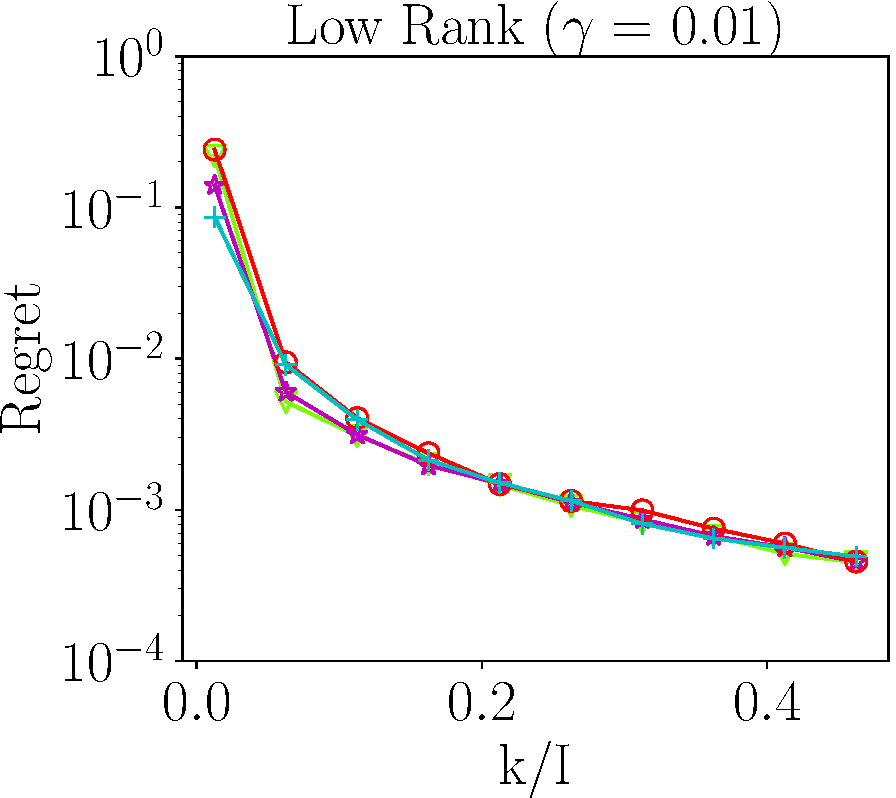
\includegraphics[scale = 0.24]{figure/fig2_lk_lnoise_400.pdf}
	\end{subfigure}
	\begin{subfigure}{0.3\textwidth}
		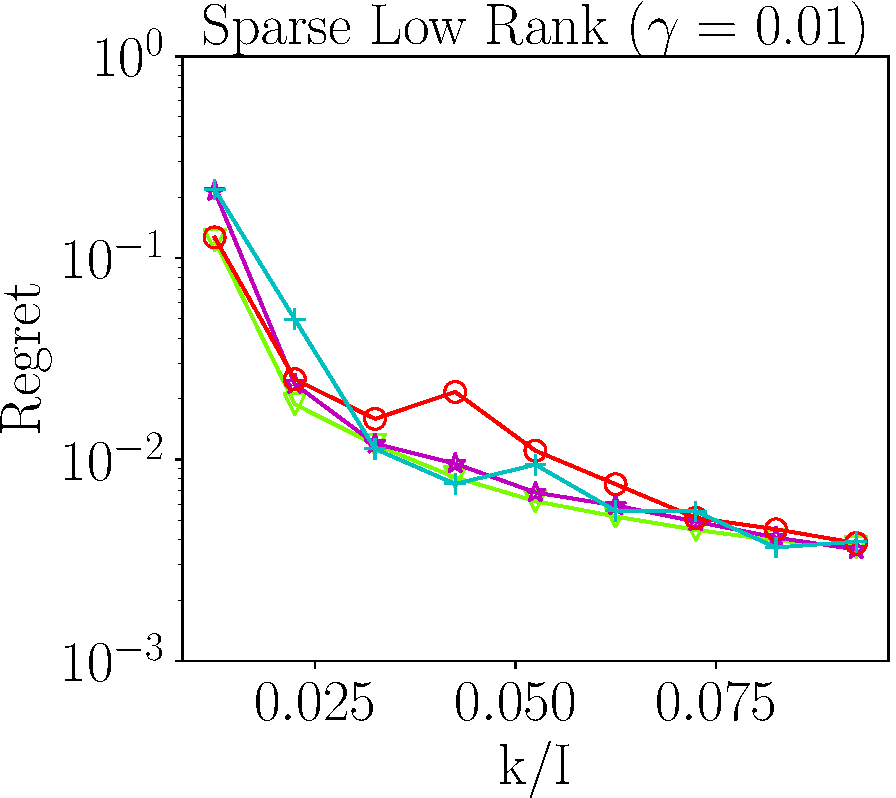
\includegraphics[scale = 0.24]{figure/fig2_slk_lnoise_400.pdf}
	\end{subfigure}
	\begin{subfigure}{0.3\textwidth}
		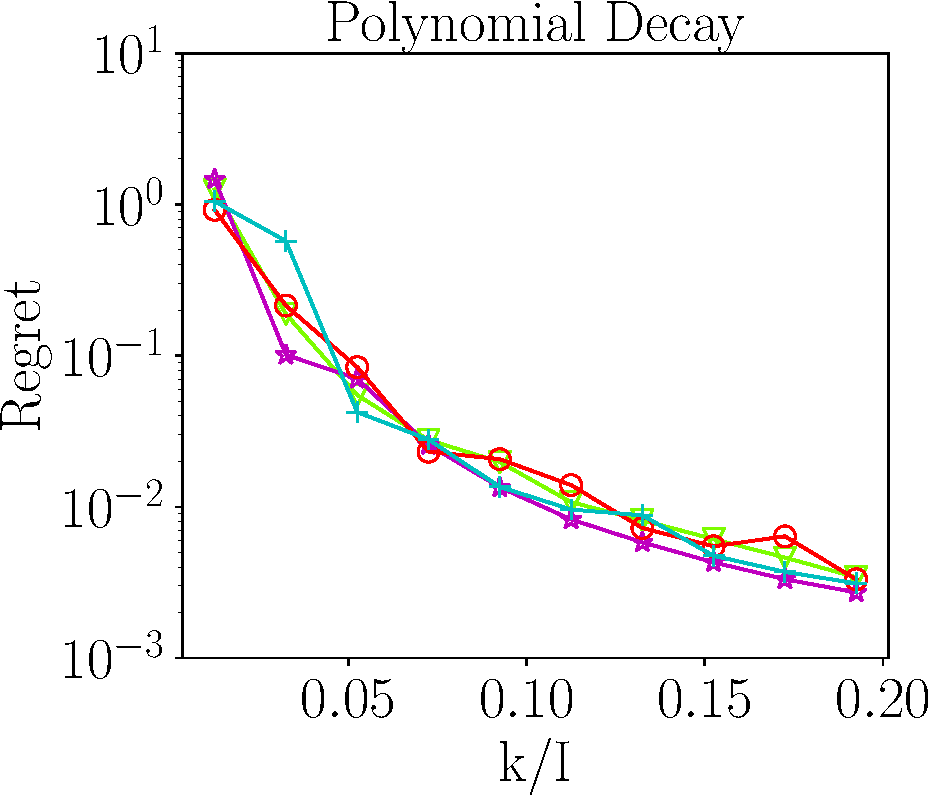
\includegraphics[scale = 0.24]{figure/fig2_spd_400.pdf}
	\end{subfigure}\\
	\begin{subfigure}{0.3\textwidth}
		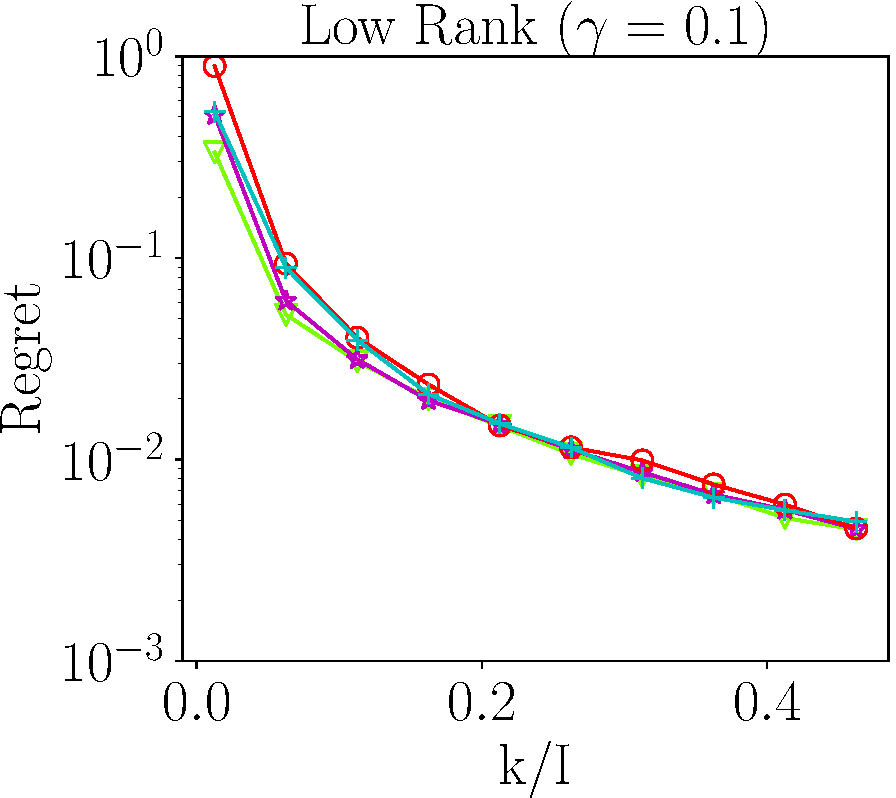
\includegraphics[scale = 0.24]{figure/fig2_lk_mnoise_400.pdf}
	\end{subfigure}
	\begin{subfigure}{0.5\textwidth}
		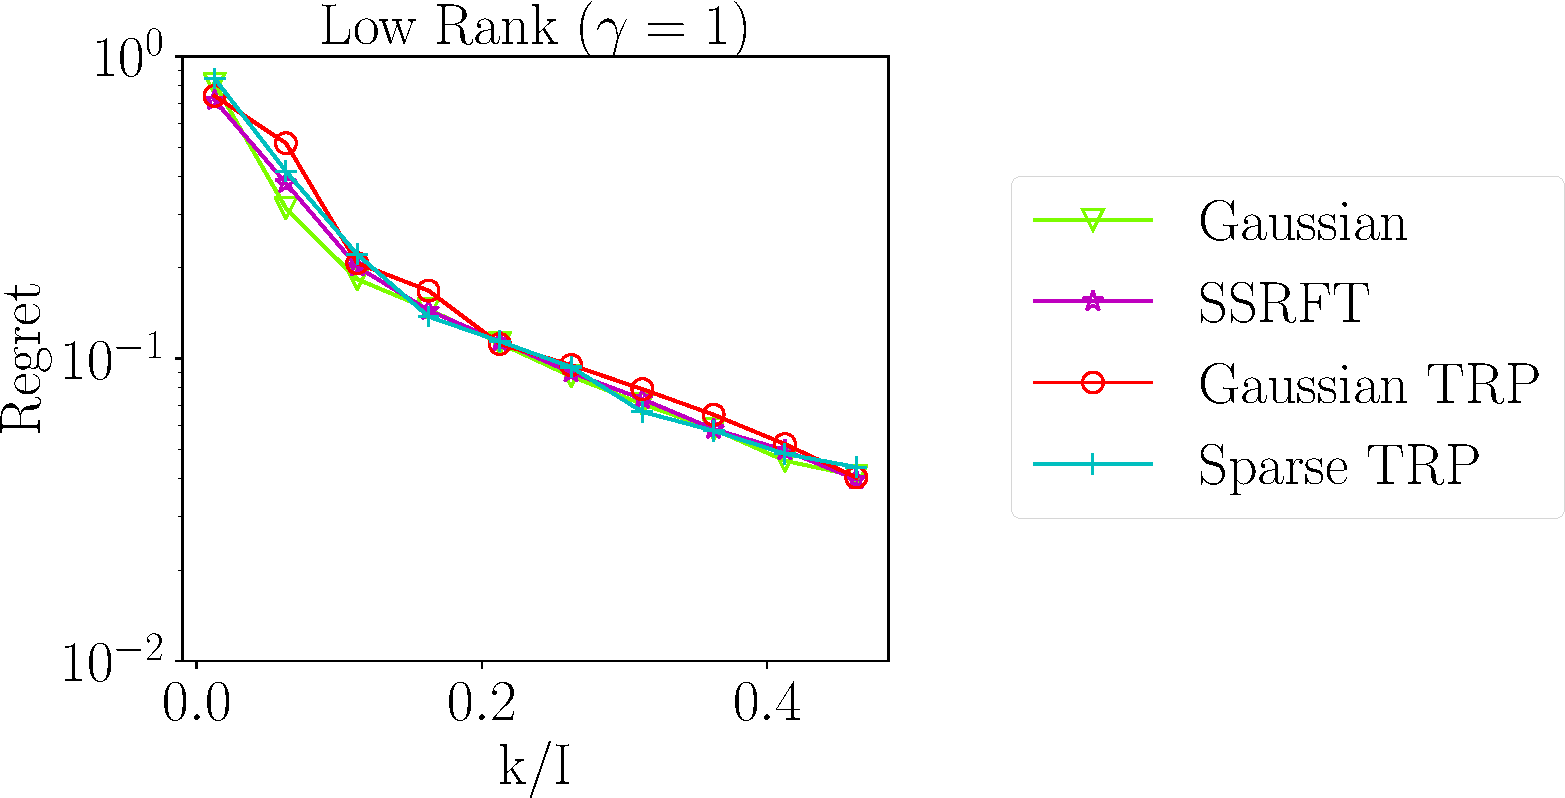
\includegraphics[scale = 0.24]{figure/fig2_lk_hnoise_400.pdf}
	\end{subfigure}
	\caption{We approximate 3D synthetic tensors (see \ref{s-synthetic-data}) with $I = 400$,
		using our one-pass algorithm with $r = 5$ and varying $k$ ($s = 2k+1$),
		using a variety of DRMs in the Tucker sketch:
		Gaussian, SSRFT, Gaussian TRP, or Sparse TRP.}
		\label{fig:vary-k-400-app}
\end{figure}



\begin{figure}
	\centering
	\begin{subfigure}{0.3\textwidth}
		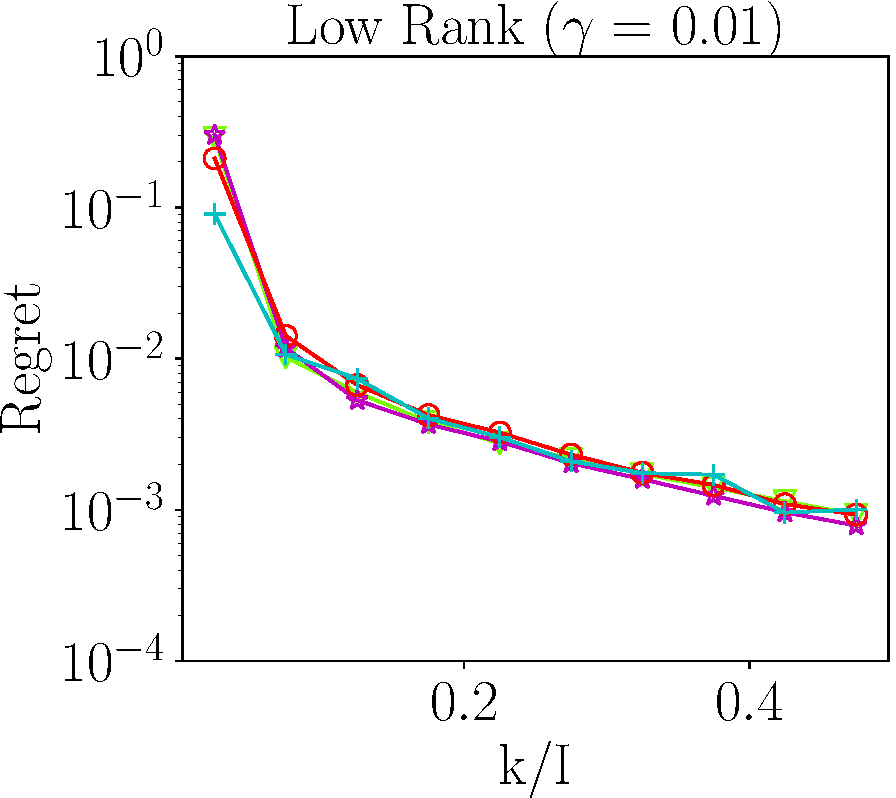
\includegraphics[scale = 0.25]{figure/fig2_lk_lnoise_200.pdf}
	\end{subfigure}
	\begin{subfigure}{0.3\textwidth}
		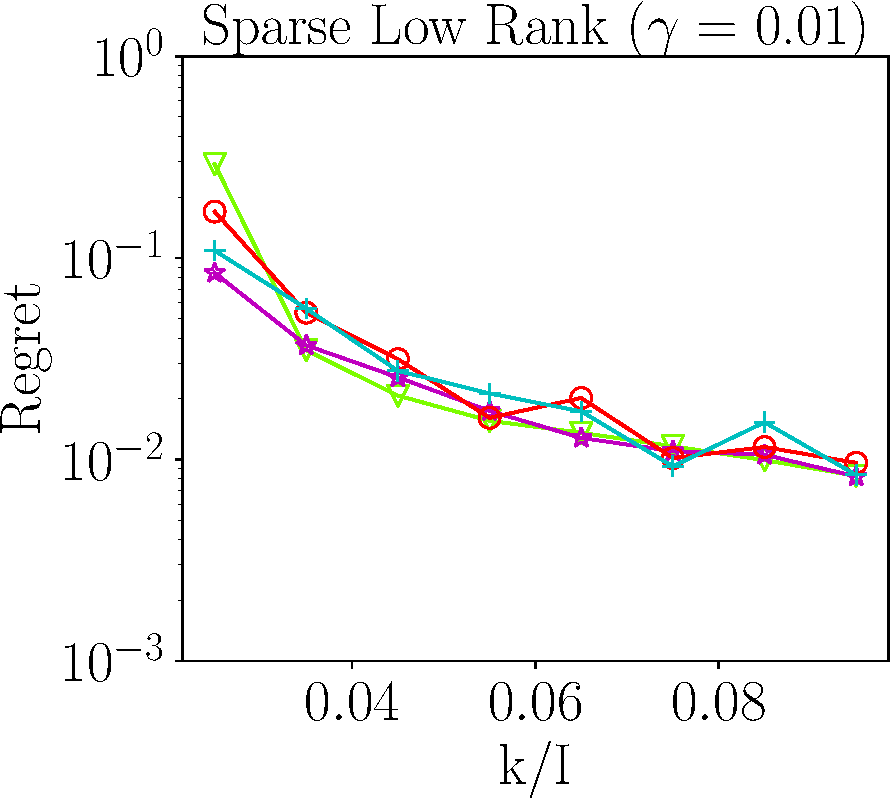
\includegraphics[scale = 0.25]{figure/fig2_slk_lnoise_200.pdf}
	\end{subfigure}
	\begin{subfigure}{0.3\textwidth}
		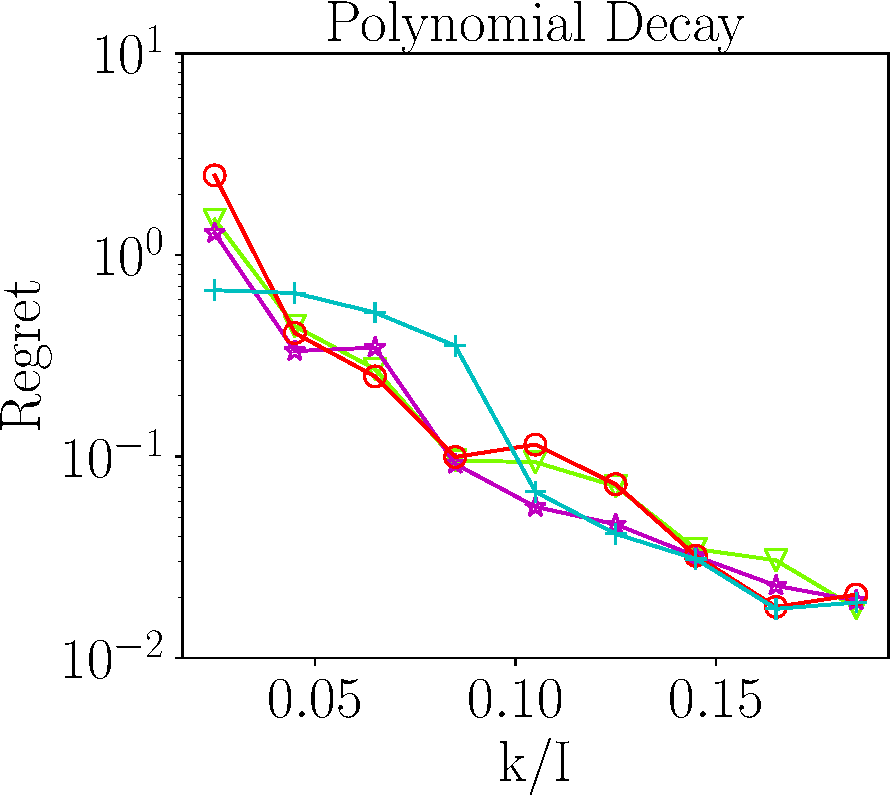
\includegraphics[scale = 0.25]{figure/fig2_spd_200.pdf}
	\end{subfigure}\\
	\begin{subfigure}{0.3\textwidth}
	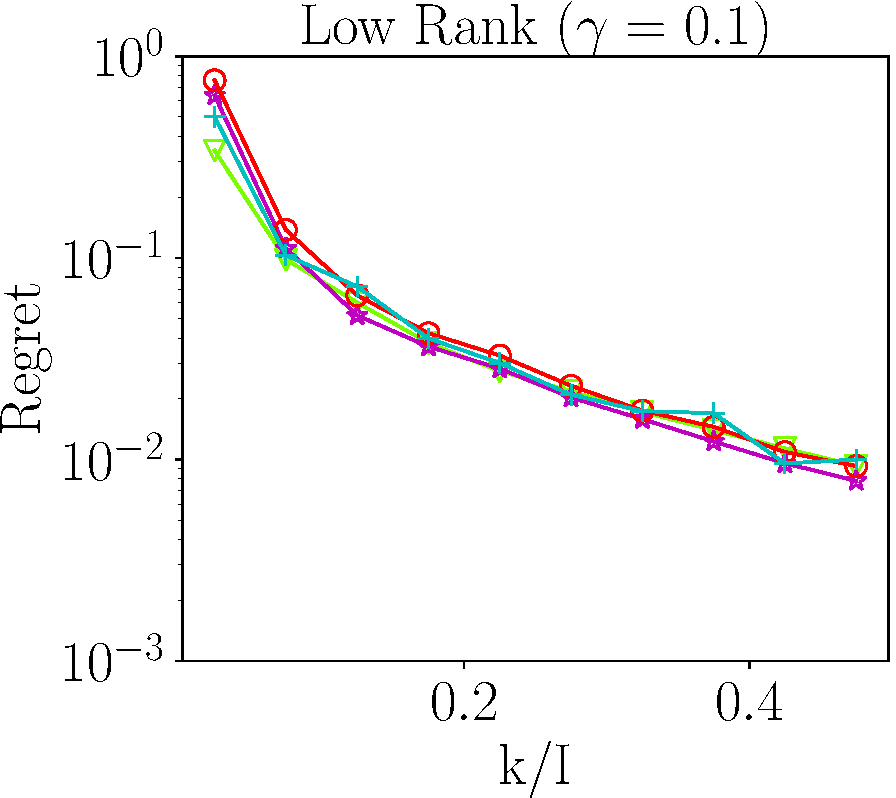
\includegraphics[scale = 0.25]{figure/fig2_lk_mnoise_200.pdf}
	\end{subfigure}
	\begin{subfigure}{0.55\textwidth}
		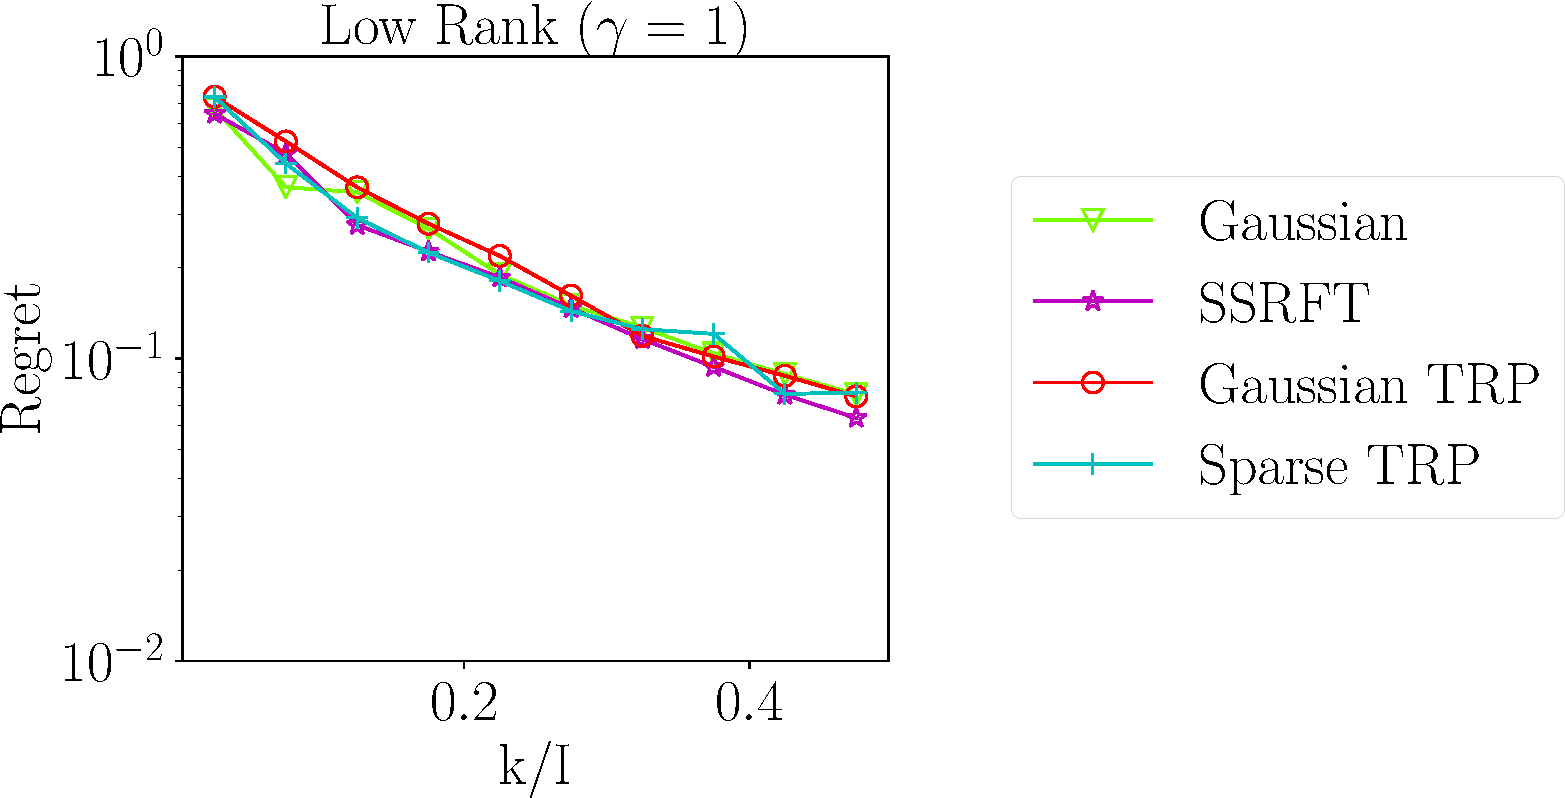
\includegraphics[scale = 0.25]{figure/fig2_lk_hnoise_200.pdf}
	\end{subfigure}
	\caption{We approximate 3D synthetic tensors (see \ref{s-synthetic-data}) with $I = 200$,
		using our one-pass algorithm with $r = 5$ and varying $k$ ($s = 2k+1$),
		using a variety of DRMs in the Tucker sketch:
		Gaussian, SSRFT, Gaussian TRP, or Sparse TRP.}
		\label{fig:vary-k-200-app}
\end{figure}

% More comparison for two-pass and one-pass algorithm


\begin{figure}
	\centering
	\begin{subfigure}{0.3\textwidth}
		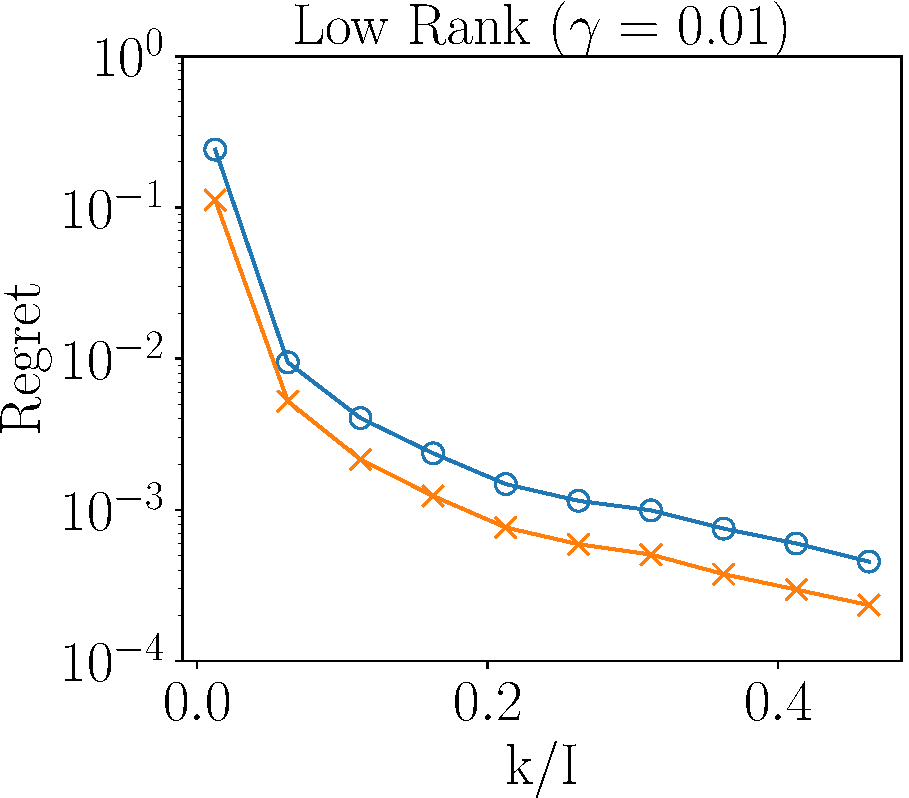
\includegraphics[scale = 0.24]{figure/fig3_lk_lnoise_400.pdf}
	\end{subfigure}
	\begin{subfigure}{0.3\textwidth}
		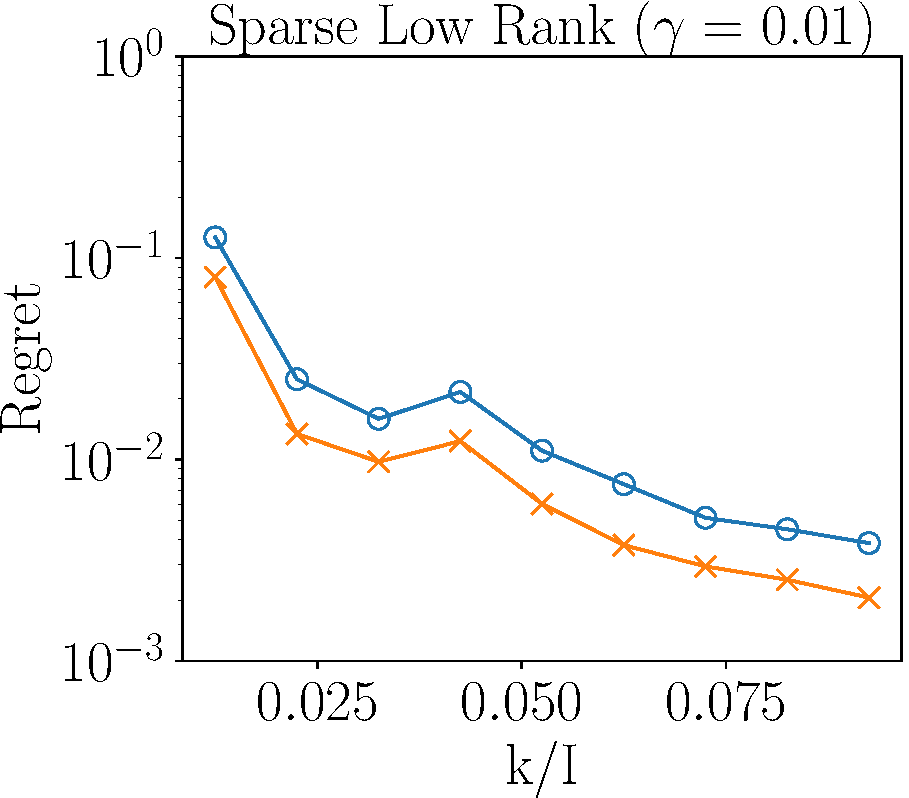
\includegraphics[scale = 0.24]{figure/fig3_slk_lnoise_400.pdf}
	\end{subfigure}
	\begin{subfigure}{0.3\textwidth}
		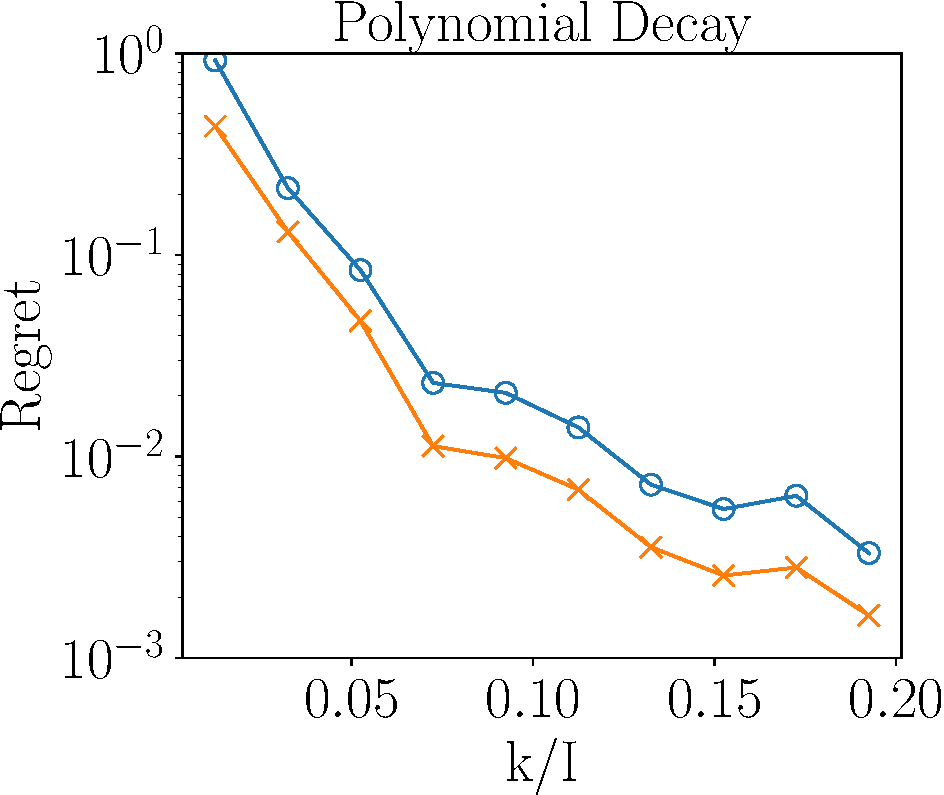
\includegraphics[scale = 0.24]{figure/fig3_spd_400.pdf}
	\end{subfigure}\\
	\begin{subfigure}{0.3\textwidth}
		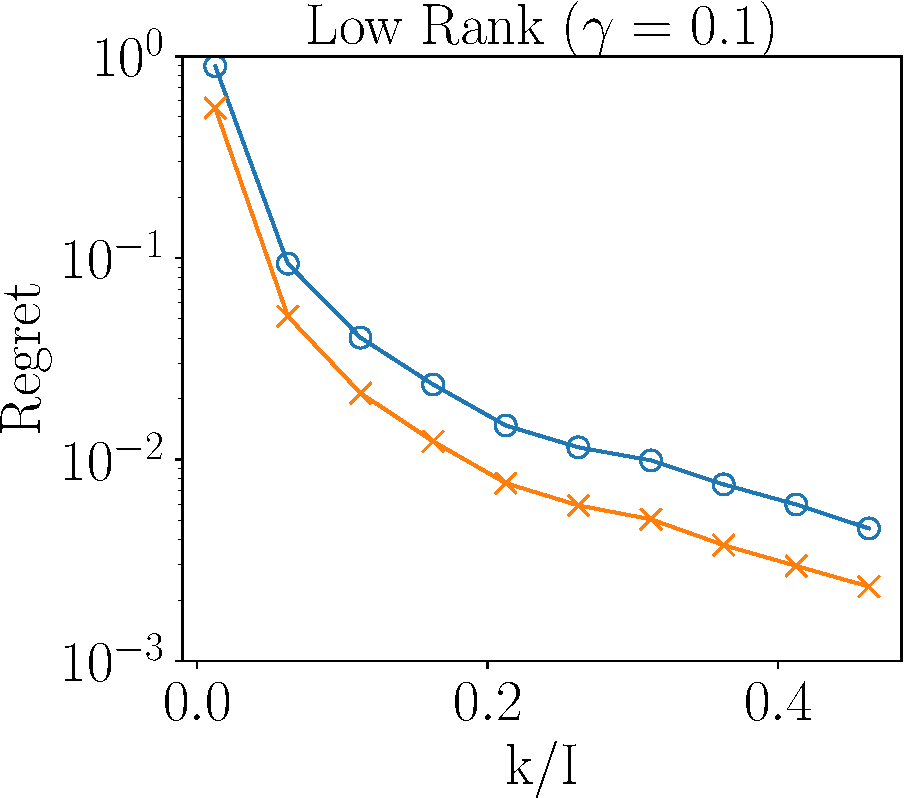
\includegraphics[scale = 0.24]{figure/fig3_lk_mnoise_400.pdf}
	\end{subfigure}
	\begin{subfigure}{0.55\textwidth}
		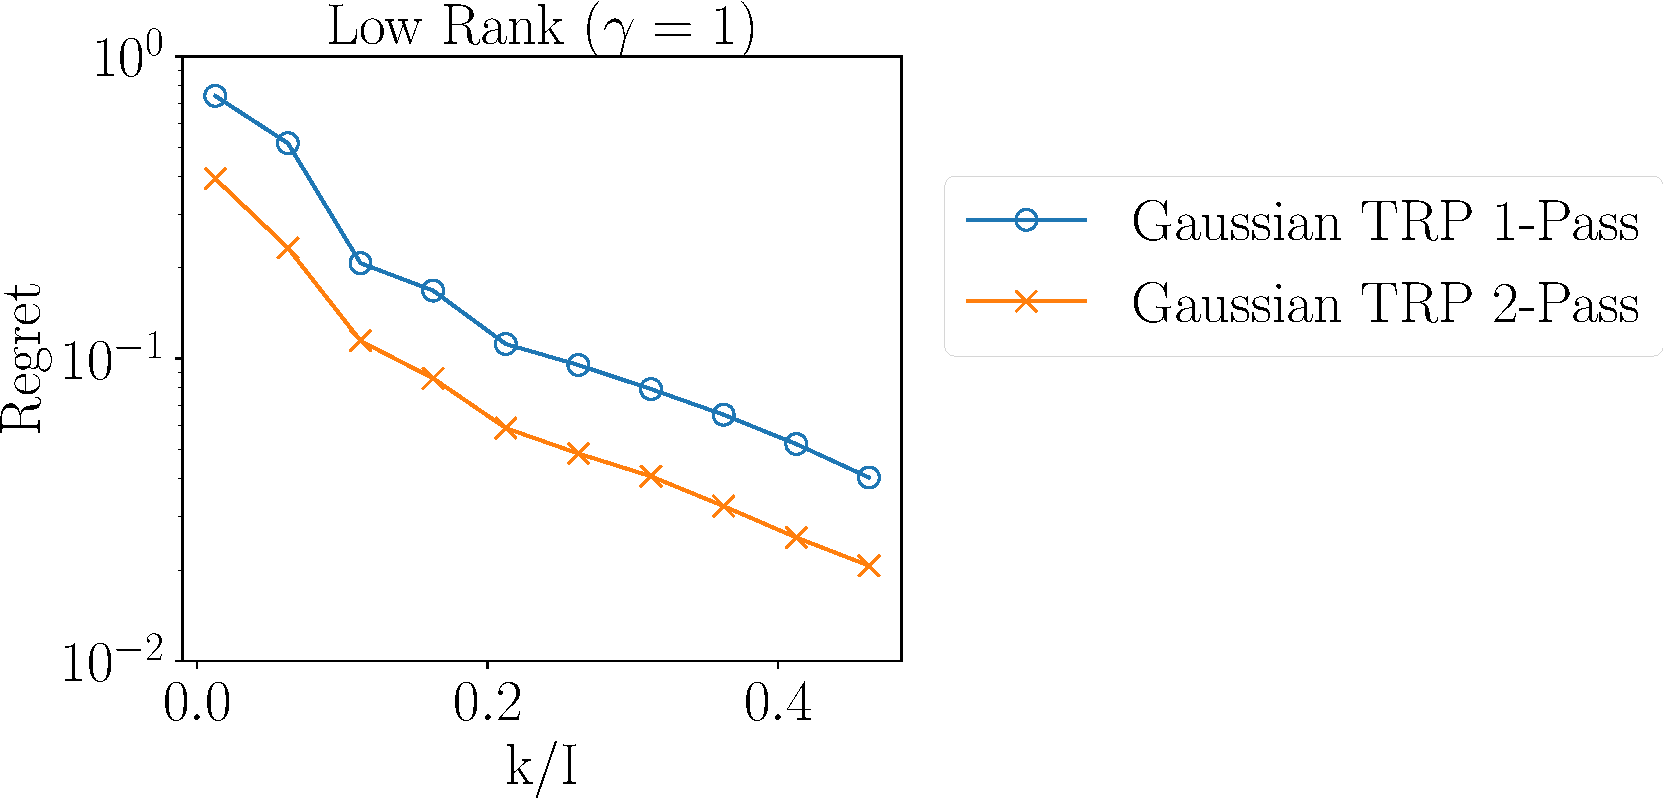
\includegraphics[scale = 0.24]{figure/fig3_lk_hnoise_400.pdf}
	\end{subfigure}
	\caption{We approximate 3D synthetic tensors (see \ref{s-synthetic-data}) with $I = 400$,
		using our one-pass and two-pass algorithms with $r = 5$ and varying $k$ ($s = 2k+1$),
		using the Gaussian TRP in the Tucker sketch.}\label{fig:vary-k-400-compare-app}
\end{figure}



\begin{figure}
	\centering
	\begin{subfigure}{0.3\textwidth}
		\includegraphics[scale = 0.25]{figure/fig3_lk_lnoise_200.pdf}
	\end{subfigure}
	\begin{subfigure}{0.3\textwidth}
		\includegraphics[scale = 0.25]{figure/fig3_slk_lnoise_200.pdf}
	\end{subfigure}
	\begin{subfigure}{0.3\textwidth}
		\includegraphics[scale = 0.25]{figure/fig3_spd_200.pdf}
	\end{subfigure}\\
	\begin{subfigure}{0.3\textwidth}
		\includegraphics[scale = 0.25]{figure/fig3_lk_mnoise_200.pdf}
	\end{subfigure}
	\begin{subfigure}{0.55\textwidth}
		\includegraphics[scale = 0.25]{figure/fig3_lk_hnoise_200.pdf}
	\end{subfigure}
	\caption{We approximate 3D synthetic tensors (see \ref{s-synthetic-data}) with $I = 200$,
		using our one-pass and two-pass algorithms with $r = 5$ and varying $k$ ($s = 2k+1$),
		using the Gaussian TRP in the Tucker sketch.}\label{fig:vary-k-200-compare-app}

\end{figure}

% \section{More Real Data Results}
\label{appendix:more_real_data_result}

We also provide more numerical results on real datasets in Figure \ref{fig:srfrad_burden_dust}.
\begin{figure}[ht]
	\centering
	\includegraphics[height=2.9cm]{figure/multi_SRFRAD_frk8.pdf}
	\includegraphics[height=2.9cm]{figure/multi_SRFRAD_frk10.pdf}
	\includegraphics[height=2.9cm]{figure/multi_SRFRAD_frk15.pdf}\\
	\textbf{Net Radiative Flux at Surface}\\~\\
	\centering
	\includegraphics[height=2.9cm]{figure/multi_BURDENDUST_frk8.pdf}
	\includegraphics[height=2.9cm]{figure/multi_BURDENDUST_frk10.pdf}
	\includegraphics[height=2.9cm]{figure/multi_BURDENDUST_frk15.pdf}\\
	\textbf{Dust Aerosol Burden}
	\caption{We approximate the net radiative flux and dust aerosol burden data using our one-pass and two-pass algorithms using Gaussian TRP. We compare the performance under different ranks ($r/I = 0.125,0.2,0.067$). The dataset comes from the CESM CAM. The dust aerosol burden measures the amount of aerosol contributed by the dust. The net radiative flux determines the energy received by the earth surface through radiation. } \label{fig:srfrad_burden_dust}
\end{figure}

\end{appendices}

\end{document}
